\documentclass[11pt]{article}

    \usepackage[breakable]{tcolorbox}
    \usepackage{parskip} % Stop auto-indenting (to mimic markdown behaviour)
    

    % Basic figure setup, for now with no caption control since it's done
    % automatically by Pandoc (which extracts ![](path) syntax from Markdown).
    \usepackage{graphicx}
    % Maintain compatibility with old templates. Remove in nbconvert 6.0
    \let\Oldincludegraphics\includegraphics
    % Ensure that by default, figures have no caption (until we provide a
    % proper Figure object with a Caption API and a way to capture that
    % in the conversion process - todo).
    \usepackage{caption}
    \DeclareCaptionFormat{nocaption}{}
    \captionsetup{format=nocaption,aboveskip=0pt,belowskip=0pt}

    \usepackage{float}
    \floatplacement{figure}{H} % forces figures to be placed at the correct location
    \usepackage{xcolor} % Allow colors to be defined
    \usepackage{enumerate} % Needed for markdown enumerations to work
    \usepackage{geometry} % Used to adjust the document margins
    \usepackage{amsmath} % Equations
    \usepackage{amssymb} % Equations
    \usepackage{textcomp} % defines textquotesingle
    % Hack from http://tex.stackexchange.com/a/47451/13684:
    \AtBeginDocument{%
        \def\PYZsq{\textquotesingle}% Upright quotes in Pygmentized code
    }
    \usepackage{upquote} % Upright quotes for verbatim code
    \usepackage{eurosym} % defines \euro

    \usepackage{iftex}
    \ifPDFTeX
        \usepackage[T1]{fontenc}
        \IfFileExists{alphabeta.sty}{
              \usepackage{alphabeta}
          }{
              \usepackage[mathletters]{ucs}
              \usepackage[utf8x]{inputenc}
          }
    \else
        \usepackage{fontspec}
        \usepackage{unicode-math}
    \fi

    \usepackage{fancyvrb} % verbatim replacement that allows latex
    \usepackage{grffile} % extends the file name processing of package graphics
                         % to support a larger range
    \makeatletter % fix for old versions of grffile with XeLaTeX
    \@ifpackagelater{grffile}{2019/11/01}
    {
      % Do nothing on new versions
    }
    {
      \def\Gread@@xetex#1{%
        \IfFileExists{"\Gin@base".bb}%
        {\Gread@eps{\Gin@base.bb}}%
        {\Gread@@xetex@aux#1}%
      }
    }
    \makeatother
    \usepackage[Export]{adjustbox} % Used to constrain images to a maximum size
    \adjustboxset{max size={0.9\linewidth}{0.9\paperheight}}

    % The hyperref package gives us a pdf with properly built
    % internal navigation ('pdf bookmarks' for the table of contents,
    % internal cross-reference links, web links for URLs, etc.)
    \usepackage{hyperref}
    % The default LaTeX title has an obnoxious amount of whitespace. By default,
    % titling removes some of it. It also provides customization options.
    \usepackage{titling}
    \usepackage{longtable} % longtable support required by pandoc >1.10
    \usepackage{booktabs}  % table support for pandoc > 1.12.2
    \usepackage{array}     % table support for pandoc >= 2.11.3
    \usepackage{calc}      % table minipage width calculation for pandoc >= 2.11.1
    \usepackage[inline]{enumitem} % IRkernel/repr support (it uses the enumerate* environment)
    \usepackage[normalem]{ulem} % ulem is needed to support strikethroughs (\sout)
                                % normalem makes italics be italics, not underlines
    \usepackage{soul}      % strikethrough (\st) support for pandoc >= 3.0.0
    \usepackage{mathrsfs}
    

    
    % Colors for the hyperref package
    \definecolor{urlcolor}{rgb}{0,.145,.698}
    \definecolor{linkcolor}{rgb}{.71,0.21,0.01}
    \definecolor{citecolor}{rgb}{.12,.54,.11}

    % ANSI colors
    \definecolor{ansi-black}{HTML}{3E424D}
    \definecolor{ansi-black-intense}{HTML}{282C36}
    \definecolor{ansi-red}{HTML}{E75C58}
    \definecolor{ansi-red-intense}{HTML}{B22B31}
    \definecolor{ansi-green}{HTML}{00A250}
    \definecolor{ansi-green-intense}{HTML}{007427}
    \definecolor{ansi-yellow}{HTML}{DDB62B}
    \definecolor{ansi-yellow-intense}{HTML}{B27D12}
    \definecolor{ansi-blue}{HTML}{208FFB}
    \definecolor{ansi-blue-intense}{HTML}{0065CA}
    \definecolor{ansi-magenta}{HTML}{D160C4}
    \definecolor{ansi-magenta-intense}{HTML}{A03196}
    \definecolor{ansi-cyan}{HTML}{60C6C8}
    \definecolor{ansi-cyan-intense}{HTML}{258F8F}
    \definecolor{ansi-white}{HTML}{C5C1B4}
    \definecolor{ansi-white-intense}{HTML}{A1A6B2}
    \definecolor{ansi-default-inverse-fg}{HTML}{FFFFFF}
    \definecolor{ansi-default-inverse-bg}{HTML}{000000}

    % common color for the border for error outputs.
    \definecolor{outerrorbackground}{HTML}{FFDFDF}

    % commands and environments needed by pandoc snippets
    % extracted from the output of `pandoc -s`
    \providecommand{\tightlist}{%
      \setlength{\itemsep}{0pt}\setlength{\parskip}{0pt}}
    \DefineVerbatimEnvironment{Highlighting}{Verbatim}{commandchars=\\\{\}}
    % Add ',fontsize=\small' for more characters per line
    \newenvironment{Shaded}{}{}
    \newcommand{\KeywordTok}[1]{\textcolor[rgb]{0.00,0.44,0.13}{\textbf{{#1}}}}
    \newcommand{\DataTypeTok}[1]{\textcolor[rgb]{0.56,0.13,0.00}{{#1}}}
    \newcommand{\DecValTok}[1]{\textcolor[rgb]{0.25,0.63,0.44}{{#1}}}
    \newcommand{\BaseNTok}[1]{\textcolor[rgb]{0.25,0.63,0.44}{{#1}}}
    \newcommand{\FloatTok}[1]{\textcolor[rgb]{0.25,0.63,0.44}{{#1}}}
    \newcommand{\CharTok}[1]{\textcolor[rgb]{0.25,0.44,0.63}{{#1}}}
    \newcommand{\StringTok}[1]{\textcolor[rgb]{0.25,0.44,0.63}{{#1}}}
    \newcommand{\CommentTok}[1]{\textcolor[rgb]{0.38,0.63,0.69}{\textit{{#1}}}}
    \newcommand{\OtherTok}[1]{\textcolor[rgb]{0.00,0.44,0.13}{{#1}}}
    \newcommand{\AlertTok}[1]{\textcolor[rgb]{1.00,0.00,0.00}{\textbf{{#1}}}}
    \newcommand{\FunctionTok}[1]{\textcolor[rgb]{0.02,0.16,0.49}{{#1}}}
    \newcommand{\RegionMarkerTok}[1]{{#1}}
    \newcommand{\ErrorTok}[1]{\textcolor[rgb]{1.00,0.00,0.00}{\textbf{{#1}}}}
    \newcommand{\NormalTok}[1]{{#1}}

    % Additional commands for more recent versions of Pandoc
    \newcommand{\ConstantTok}[1]{\textcolor[rgb]{0.53,0.00,0.00}{{#1}}}
    \newcommand{\SpecialCharTok}[1]{\textcolor[rgb]{0.25,0.44,0.63}{{#1}}}
    \newcommand{\VerbatimStringTok}[1]{\textcolor[rgb]{0.25,0.44,0.63}{{#1}}}
    \newcommand{\SpecialStringTok}[1]{\textcolor[rgb]{0.73,0.40,0.53}{{#1}}}
    \newcommand{\ImportTok}[1]{{#1}}
    \newcommand{\DocumentationTok}[1]{\textcolor[rgb]{0.73,0.13,0.13}{\textit{{#1}}}}
    \newcommand{\AnnotationTok}[1]{\textcolor[rgb]{0.38,0.63,0.69}{\textbf{\textit{{#1}}}}}
    \newcommand{\CommentVarTok}[1]{\textcolor[rgb]{0.38,0.63,0.69}{\textbf{\textit{{#1}}}}}
    \newcommand{\VariableTok}[1]{\textcolor[rgb]{0.10,0.09,0.49}{{#1}}}
    \newcommand{\ControlFlowTok}[1]{\textcolor[rgb]{0.00,0.44,0.13}{\textbf{{#1}}}}
    \newcommand{\OperatorTok}[1]{\textcolor[rgb]{0.40,0.40,0.40}{{#1}}}
    \newcommand{\BuiltInTok}[1]{{#1}}
    \newcommand{\ExtensionTok}[1]{{#1}}
    \newcommand{\PreprocessorTok}[1]{\textcolor[rgb]{0.74,0.48,0.00}{{#1}}}
    \newcommand{\AttributeTok}[1]{\textcolor[rgb]{0.49,0.56,0.16}{{#1}}}
    \newcommand{\InformationTok}[1]{\textcolor[rgb]{0.38,0.63,0.69}{\textbf{\textit{{#1}}}}}
    \newcommand{\WarningTok}[1]{\textcolor[rgb]{0.38,0.63,0.69}{\textbf{\textit{{#1}}}}}


    % Define a nice break command that doesn't care if a line doesn't already
    % exist.
    \def\br{\hspace*{\fill} \\* }
    % Math Jax compatibility definitions
    \def\gt{>}
    \def\lt{<}
    \let\Oldtex\TeX
    \let\Oldlatex\LaTeX
    \renewcommand{\TeX}{\textrm{\Oldtex}}
    \renewcommand{\LaTeX}{\textrm{\Oldlatex}}
    % Document parameters
    % Document title
    \title{multi\_shrna\_screening\_ap009}
    
    
    
    
    
    
    
% Pygments definitions
\makeatletter
\def\PY@reset{\let\PY@it=\relax \let\PY@bf=\relax%
    \let\PY@ul=\relax \let\PY@tc=\relax%
    \let\PY@bc=\relax \let\PY@ff=\relax}
\def\PY@tok#1{\csname PY@tok@#1\endcsname}
\def\PY@toks#1+{\ifx\relax#1\empty\else%
    \PY@tok{#1}\expandafter\PY@toks\fi}
\def\PY@do#1{\PY@bc{\PY@tc{\PY@ul{%
    \PY@it{\PY@bf{\PY@ff{#1}}}}}}}
\def\PY#1#2{\PY@reset\PY@toks#1+\relax+\PY@do{#2}}

\@namedef{PY@tok@w}{\def\PY@tc##1{\textcolor[rgb]{0.73,0.73,0.73}{##1}}}
\@namedef{PY@tok@c}{\let\PY@it=\textit\def\PY@tc##1{\textcolor[rgb]{0.24,0.48,0.48}{##1}}}
\@namedef{PY@tok@cp}{\def\PY@tc##1{\textcolor[rgb]{0.61,0.40,0.00}{##1}}}
\@namedef{PY@tok@k}{\let\PY@bf=\textbf\def\PY@tc##1{\textcolor[rgb]{0.00,0.50,0.00}{##1}}}
\@namedef{PY@tok@kp}{\def\PY@tc##1{\textcolor[rgb]{0.00,0.50,0.00}{##1}}}
\@namedef{PY@tok@kt}{\def\PY@tc##1{\textcolor[rgb]{0.69,0.00,0.25}{##1}}}
\@namedef{PY@tok@o}{\def\PY@tc##1{\textcolor[rgb]{0.40,0.40,0.40}{##1}}}
\@namedef{PY@tok@ow}{\let\PY@bf=\textbf\def\PY@tc##1{\textcolor[rgb]{0.67,0.13,1.00}{##1}}}
\@namedef{PY@tok@nb}{\def\PY@tc##1{\textcolor[rgb]{0.00,0.50,0.00}{##1}}}
\@namedef{PY@tok@nf}{\def\PY@tc##1{\textcolor[rgb]{0.00,0.00,1.00}{##1}}}
\@namedef{PY@tok@nc}{\let\PY@bf=\textbf\def\PY@tc##1{\textcolor[rgb]{0.00,0.00,1.00}{##1}}}
\@namedef{PY@tok@nn}{\let\PY@bf=\textbf\def\PY@tc##1{\textcolor[rgb]{0.00,0.00,1.00}{##1}}}
\@namedef{PY@tok@ne}{\let\PY@bf=\textbf\def\PY@tc##1{\textcolor[rgb]{0.80,0.25,0.22}{##1}}}
\@namedef{PY@tok@nv}{\def\PY@tc##1{\textcolor[rgb]{0.10,0.09,0.49}{##1}}}
\@namedef{PY@tok@no}{\def\PY@tc##1{\textcolor[rgb]{0.53,0.00,0.00}{##1}}}
\@namedef{PY@tok@nl}{\def\PY@tc##1{\textcolor[rgb]{0.46,0.46,0.00}{##1}}}
\@namedef{PY@tok@ni}{\let\PY@bf=\textbf\def\PY@tc##1{\textcolor[rgb]{0.44,0.44,0.44}{##1}}}
\@namedef{PY@tok@na}{\def\PY@tc##1{\textcolor[rgb]{0.41,0.47,0.13}{##1}}}
\@namedef{PY@tok@nt}{\let\PY@bf=\textbf\def\PY@tc##1{\textcolor[rgb]{0.00,0.50,0.00}{##1}}}
\@namedef{PY@tok@nd}{\def\PY@tc##1{\textcolor[rgb]{0.67,0.13,1.00}{##1}}}
\@namedef{PY@tok@s}{\def\PY@tc##1{\textcolor[rgb]{0.73,0.13,0.13}{##1}}}
\@namedef{PY@tok@sd}{\let\PY@it=\textit\def\PY@tc##1{\textcolor[rgb]{0.73,0.13,0.13}{##1}}}
\@namedef{PY@tok@si}{\let\PY@bf=\textbf\def\PY@tc##1{\textcolor[rgb]{0.64,0.35,0.47}{##1}}}
\@namedef{PY@tok@se}{\let\PY@bf=\textbf\def\PY@tc##1{\textcolor[rgb]{0.67,0.36,0.12}{##1}}}
\@namedef{PY@tok@sr}{\def\PY@tc##1{\textcolor[rgb]{0.64,0.35,0.47}{##1}}}
\@namedef{PY@tok@ss}{\def\PY@tc##1{\textcolor[rgb]{0.10,0.09,0.49}{##1}}}
\@namedef{PY@tok@sx}{\def\PY@tc##1{\textcolor[rgb]{0.00,0.50,0.00}{##1}}}
\@namedef{PY@tok@m}{\def\PY@tc##1{\textcolor[rgb]{0.40,0.40,0.40}{##1}}}
\@namedef{PY@tok@gh}{\let\PY@bf=\textbf\def\PY@tc##1{\textcolor[rgb]{0.00,0.00,0.50}{##1}}}
\@namedef{PY@tok@gu}{\let\PY@bf=\textbf\def\PY@tc##1{\textcolor[rgb]{0.50,0.00,0.50}{##1}}}
\@namedef{PY@tok@gd}{\def\PY@tc##1{\textcolor[rgb]{0.63,0.00,0.00}{##1}}}
\@namedef{PY@tok@gi}{\def\PY@tc##1{\textcolor[rgb]{0.00,0.52,0.00}{##1}}}
\@namedef{PY@tok@gr}{\def\PY@tc##1{\textcolor[rgb]{0.89,0.00,0.00}{##1}}}
\@namedef{PY@tok@ge}{\let\PY@it=\textit}
\@namedef{PY@tok@gs}{\let\PY@bf=\textbf}
\@namedef{PY@tok@gp}{\let\PY@bf=\textbf\def\PY@tc##1{\textcolor[rgb]{0.00,0.00,0.50}{##1}}}
\@namedef{PY@tok@go}{\def\PY@tc##1{\textcolor[rgb]{0.44,0.44,0.44}{##1}}}
\@namedef{PY@tok@gt}{\def\PY@tc##1{\textcolor[rgb]{0.00,0.27,0.87}{##1}}}
\@namedef{PY@tok@err}{\def\PY@bc##1{{\setlength{\fboxsep}{\string -\fboxrule}\fcolorbox[rgb]{1.00,0.00,0.00}{1,1,1}{\strut ##1}}}}
\@namedef{PY@tok@kc}{\let\PY@bf=\textbf\def\PY@tc##1{\textcolor[rgb]{0.00,0.50,0.00}{##1}}}
\@namedef{PY@tok@kd}{\let\PY@bf=\textbf\def\PY@tc##1{\textcolor[rgb]{0.00,0.50,0.00}{##1}}}
\@namedef{PY@tok@kn}{\let\PY@bf=\textbf\def\PY@tc##1{\textcolor[rgb]{0.00,0.50,0.00}{##1}}}
\@namedef{PY@tok@kr}{\let\PY@bf=\textbf\def\PY@tc##1{\textcolor[rgb]{0.00,0.50,0.00}{##1}}}
\@namedef{PY@tok@bp}{\def\PY@tc##1{\textcolor[rgb]{0.00,0.50,0.00}{##1}}}
\@namedef{PY@tok@fm}{\def\PY@tc##1{\textcolor[rgb]{0.00,0.00,1.00}{##1}}}
\@namedef{PY@tok@vc}{\def\PY@tc##1{\textcolor[rgb]{0.10,0.09,0.49}{##1}}}
\@namedef{PY@tok@vg}{\def\PY@tc##1{\textcolor[rgb]{0.10,0.09,0.49}{##1}}}
\@namedef{PY@tok@vi}{\def\PY@tc##1{\textcolor[rgb]{0.10,0.09,0.49}{##1}}}
\@namedef{PY@tok@vm}{\def\PY@tc##1{\textcolor[rgb]{0.10,0.09,0.49}{##1}}}
\@namedef{PY@tok@sa}{\def\PY@tc##1{\textcolor[rgb]{0.73,0.13,0.13}{##1}}}
\@namedef{PY@tok@sb}{\def\PY@tc##1{\textcolor[rgb]{0.73,0.13,0.13}{##1}}}
\@namedef{PY@tok@sc}{\def\PY@tc##1{\textcolor[rgb]{0.73,0.13,0.13}{##1}}}
\@namedef{PY@tok@dl}{\def\PY@tc##1{\textcolor[rgb]{0.73,0.13,0.13}{##1}}}
\@namedef{PY@tok@s2}{\def\PY@tc##1{\textcolor[rgb]{0.73,0.13,0.13}{##1}}}
\@namedef{PY@tok@sh}{\def\PY@tc##1{\textcolor[rgb]{0.73,0.13,0.13}{##1}}}
\@namedef{PY@tok@s1}{\def\PY@tc##1{\textcolor[rgb]{0.73,0.13,0.13}{##1}}}
\@namedef{PY@tok@mb}{\def\PY@tc##1{\textcolor[rgb]{0.40,0.40,0.40}{##1}}}
\@namedef{PY@tok@mf}{\def\PY@tc##1{\textcolor[rgb]{0.40,0.40,0.40}{##1}}}
\@namedef{PY@tok@mh}{\def\PY@tc##1{\textcolor[rgb]{0.40,0.40,0.40}{##1}}}
\@namedef{PY@tok@mi}{\def\PY@tc##1{\textcolor[rgb]{0.40,0.40,0.40}{##1}}}
\@namedef{PY@tok@il}{\def\PY@tc##1{\textcolor[rgb]{0.40,0.40,0.40}{##1}}}
\@namedef{PY@tok@mo}{\def\PY@tc##1{\textcolor[rgb]{0.40,0.40,0.40}{##1}}}
\@namedef{PY@tok@ch}{\let\PY@it=\textit\def\PY@tc##1{\textcolor[rgb]{0.24,0.48,0.48}{##1}}}
\@namedef{PY@tok@cm}{\let\PY@it=\textit\def\PY@tc##1{\textcolor[rgb]{0.24,0.48,0.48}{##1}}}
\@namedef{PY@tok@cpf}{\let\PY@it=\textit\def\PY@tc##1{\textcolor[rgb]{0.24,0.48,0.48}{##1}}}
\@namedef{PY@tok@c1}{\let\PY@it=\textit\def\PY@tc##1{\textcolor[rgb]{0.24,0.48,0.48}{##1}}}
\@namedef{PY@tok@cs}{\let\PY@it=\textit\def\PY@tc##1{\textcolor[rgb]{0.24,0.48,0.48}{##1}}}

\def\PYZbs{\char`\\}
\def\PYZus{\char`\_}
\def\PYZob{\char`\{}
\def\PYZcb{\char`\}}
\def\PYZca{\char`\^}
\def\PYZam{\char`\&}
\def\PYZlt{\char`\<}
\def\PYZgt{\char`\>}
\def\PYZsh{\char`\#}
\def\PYZpc{\char`\%}
\def\PYZdl{\char`\$}
\def\PYZhy{\char`\-}
\def\PYZsq{\char`\'}
\def\PYZdq{\char`\"}
\def\PYZti{\char`\~}
% for compatibility with earlier versions
\def\PYZat{@}
\def\PYZlb{[}
\def\PYZrb{]}
\makeatother


    % For linebreaks inside Verbatim environment from package fancyvrb.
    \makeatletter
        \newbox\Wrappedcontinuationbox
        \newbox\Wrappedvisiblespacebox
        \newcommand*\Wrappedvisiblespace {\textcolor{red}{\textvisiblespace}}
        \newcommand*\Wrappedcontinuationsymbol {\textcolor{red}{\llap{\tiny$\m@th\hookrightarrow$}}}
        \newcommand*\Wrappedcontinuationindent {3ex }
        \newcommand*\Wrappedafterbreak {\kern\Wrappedcontinuationindent\copy\Wrappedcontinuationbox}
        % Take advantage of the already applied Pygments mark-up to insert
        % potential linebreaks for TeX processing.
        %        {, <, #, %, $, ' and ": go to next line.
        %        _, }, ^, &, >, - and ~: stay at end of broken line.
        % Use of \textquotesingle for straight quote.
        \newcommand*\Wrappedbreaksatspecials {%
            \def\PYGZus{\discretionary{\char`\_}{\Wrappedafterbreak}{\char`\_}}%
            \def\PYGZob{\discretionary{}{\Wrappedafterbreak\char`\{}{\char`\{}}%
            \def\PYGZcb{\discretionary{\char`\}}{\Wrappedafterbreak}{\char`\}}}%
            \def\PYGZca{\discretionary{\char`\^}{\Wrappedafterbreak}{\char`\^}}%
            \def\PYGZam{\discretionary{\char`\&}{\Wrappedafterbreak}{\char`\&}}%
            \def\PYGZlt{\discretionary{}{\Wrappedafterbreak\char`\<}{\char`\<}}%
            \def\PYGZgt{\discretionary{\char`\>}{\Wrappedafterbreak}{\char`\>}}%
            \def\PYGZsh{\discretionary{}{\Wrappedafterbreak\char`\#}{\char`\#}}%
            \def\PYGZpc{\discretionary{}{\Wrappedafterbreak\char`\%}{\char`\%}}%
            \def\PYGZdl{\discretionary{}{\Wrappedafterbreak\char`\$}{\char`\$}}%
            \def\PYGZhy{\discretionary{\char`\-}{\Wrappedafterbreak}{\char`\-}}%
            \def\PYGZsq{\discretionary{}{\Wrappedafterbreak\textquotesingle}{\textquotesingle}}%
            \def\PYGZdq{\discretionary{}{\Wrappedafterbreak\char`\"}{\char`\"}}%
            \def\PYGZti{\discretionary{\char`\~}{\Wrappedafterbreak}{\char`\~}}%
        }
        % Some characters . , ; ? ! / are not pygmentized.
        % This macro makes them "active" and they will insert potential linebreaks
        \newcommand*\Wrappedbreaksatpunct {%
            \lccode`\~`\.\lowercase{\def~}{\discretionary{\hbox{\char`\.}}{\Wrappedafterbreak}{\hbox{\char`\.}}}%
            \lccode`\~`\,\lowercase{\def~}{\discretionary{\hbox{\char`\,}}{\Wrappedafterbreak}{\hbox{\char`\,}}}%
            \lccode`\~`\;\lowercase{\def~}{\discretionary{\hbox{\char`\;}}{\Wrappedafterbreak}{\hbox{\char`\;}}}%
            \lccode`\~`\:\lowercase{\def~}{\discretionary{\hbox{\char`\:}}{\Wrappedafterbreak}{\hbox{\char`\:}}}%
            \lccode`\~`\?\lowercase{\def~}{\discretionary{\hbox{\char`\?}}{\Wrappedafterbreak}{\hbox{\char`\?}}}%
            \lccode`\~`\!\lowercase{\def~}{\discretionary{\hbox{\char`\!}}{\Wrappedafterbreak}{\hbox{\char`\!}}}%
            \lccode`\~`\/\lowercase{\def~}{\discretionary{\hbox{\char`\/}}{\Wrappedafterbreak}{\hbox{\char`\/}}}%
            \catcode`\.\active
            \catcode`\,\active
            \catcode`\;\active
            \catcode`\:\active
            \catcode`\?\active
            \catcode`\!\active
            \catcode`\/\active
            \lccode`\~`\~
        }
    \makeatother

    \let\OriginalVerbatim=\Verbatim
    \makeatletter
    \renewcommand{\Verbatim}[1][1]{%
        %\parskip\z@skip
        \sbox\Wrappedcontinuationbox {\Wrappedcontinuationsymbol}%
        \sbox\Wrappedvisiblespacebox {\FV@SetupFont\Wrappedvisiblespace}%
        \def\FancyVerbFormatLine ##1{\hsize\linewidth
            \vtop{\raggedright\hyphenpenalty\z@\exhyphenpenalty\z@
                \doublehyphendemerits\z@\finalhyphendemerits\z@
                \strut ##1\strut}%
        }%
        % If the linebreak is at a space, the latter will be displayed as visible
        % space at end of first line, and a continuation symbol starts next line.
        % Stretch/shrink are however usually zero for typewriter font.
        \def\FV@Space {%
            \nobreak\hskip\z@ plus\fontdimen3\font minus\fontdimen4\font
            \discretionary{\copy\Wrappedvisiblespacebox}{\Wrappedafterbreak}
            {\kern\fontdimen2\font}%
        }%

        % Allow breaks at special characters using \PYG... macros.
        \Wrappedbreaksatspecials
        % Breaks at punctuation characters . , ; ? ! and / need catcode=\active
        \OriginalVerbatim[#1,codes*=\Wrappedbreaksatpunct]%
    }
    \makeatother

    % Exact colors from NB
    \definecolor{incolor}{HTML}{303F9F}
    \definecolor{outcolor}{HTML}{D84315}
    \definecolor{cellborder}{HTML}{CFCFCF}
    \definecolor{cellbackground}{HTML}{F7F7F7}

    % prompt
    \makeatletter
    \newcommand{\boxspacing}{\kern\kvtcb@left@rule\kern\kvtcb@boxsep}
    \makeatother
    \newcommand{\prompt}[4]{
        {\ttfamily\llap{{\color{#2}[#3]:\hspace{3pt}#4}}\vspace{-\baselineskip}}
    }
    

    
    % Prevent overflowing lines due to hard-to-break entities
    \sloppy
    % Setup hyperref package
    \hypersetup{
      breaklinks=true,  % so long urls are correctly broken across lines
      colorlinks=true,
      urlcolor=urlcolor,
      linkcolor=linkcolor,
      citecolor=citecolor,
      }
    % Slightly bigger margins than the latex defaults
    
    \geometry{verbose,tmargin=1in,bmargin=1in,lmargin=1in,rmargin=1in}
    
    

\begin{document}
    
    \maketitle
    
    

    
    \section{Multiplexed shRNA screening AP009
analytics}\label{multiplexed-shrna-screening-ap009-analytics}

Biao Li

This notebook includes analysis scripts of processing count table of
multiplexed shRNA screening experiments on AP009 cell line received from
Cellecta, and evaluating * whether multi-shRNA system works as expected
* prognostic effect of genotype X, and * predictive effect of genetype X
on response to treatment

Note - bash commands to convert notebook to pdf:

\(>\)
\texttt{jupyter\ nbconvert\ -\/-to\ latex\ multi\_shrna\_screening\_ap009.ipynb}

\(>\) \texttt{xelatex\ multi\_shrna\_screening\_ap009.tex}

    \subsection{Setup path to project
directory}\label{setup-path-to-project-directory}

This should be absolute path to where project is saved at as a git repo.

Subfolders of the project directory should be \texttt{code},
\texttt{data}, \texttt{app}, etc.

    \begin{tcolorbox}[breakable, size=fbox, boxrule=1pt, pad at break*=1mm,colback=cellbackground, colframe=cellborder]
\prompt{In}{incolor}{303}{\boxspacing}
\begin{Verbatim}[commandchars=\\\{\}]
\PY{n}{proj\PYZus{}dir} \PY{o}{=} \PY{l+s+s2}{\PYZdq{}}\PY{l+s+s2}{/Users/bli/Documents/Projects/Multi\PYZus{}shRNA\PYZus{}screening\PYZus{}AP009/}\PY{l+s+s2}{\PYZdq{}}
\end{Verbatim}
\end{tcolorbox}

    \subsection{(ToDos)}\label{todos}

\begin{itemize}
\tightlist
\item
  (Done) Add correlation plots between baseline condition and plasmid
  counts per target
\item
  (Done) Normalize raw counts to library size of each sample
\item
  (Done) Normalize representations to dox- group
\item
  (Done) log2 transform ratio of ratios such that under the alternative
  hypothesis Score != 0, a positive sign suggests that cells with a
  particular shRNA are more resistant than cells of NT shRNAs, while a
  negative sign suggests cells are more sensitive
\item
  (Done) Use nonparametric bootstrapping to derive null distribution of
  medians (among resampling 10 NT shRNAs from NT shRNA pool) and assess
  statistical significance / adjusted empirical p-values of each target
  gene

  \begin{itemize}
  \tightlist
  \item
    Prognostic effect (combine three timepoints)
  \item
    Predictive effect (combine three timepoints and two dosages, combine
    three timepoints and keep dosages separate)
  \item
    instead of boxplot, show median +/- bootstrapped CI of median,
    highlight medians of statistical significance with a bright color,
    and others with gray
  \item
    Volcano plot of adjusted p-values vs observed median effects
  \end{itemize}
\item
  (flip) Reannotate RCC (relative cell counts) as RTN (relative
  tumor-cell numbers)
\item
  (+/- Dox) Add analytics/figures similar to Fig.2 D of Ian's NatComm
  2023 paper

  \begin{itemize}
  \tightlist
  \item
    check Prognostic / predictive effects between T10 and T13
  \end{itemize}
\item
  Add analytics/figures similar to Fig.7 of Ian's NatComm 2023 paper
\item
  Assess reproducibility between two technical replicates (D18-A vs
  D18-B)
\item
  Annotated gene list

  \begin{itemize}
  \tightlist
  \item
    update control annotations
  \item
    oncokb annotations
  \item
    pathway / protein complex annotations
  \end{itemize}
\end{itemize}

    \begin{tcolorbox}[breakable, size=fbox, boxrule=1pt, pad at break*=1mm,colback=cellbackground, colframe=cellborder]
\prompt{In}{incolor}{4}{\boxspacing}
\begin{Verbatim}[commandchars=\\\{\}]
\PY{o}{!}pip\PY{+w}{ }install\PY{+w}{ }matplotlib\PYZus{}venn\PY{+w}{ }\PYZhy{}\PYZhy{}trusted\PYZhy{}host\PY{+w}{ }pypi.python.org\PY{+w}{ }\PYZhy{}\PYZhy{}trusted\PYZhy{}host\PY{+w}{ }pypi.org\PY{+w}{ }\PYZhy{}\PYZhy{}trusted\PYZhy{}host\PY{+w}{ }files.pythonhosted.org
\end{Verbatim}
\end{tcolorbox}

    \begin{Verbatim}[commandchars=\\\{\}]
Requirement already satisfied: matplotlib\_venn in
/opt/anaconda3/lib/python3.11/site-packages (1.1.2)
Requirement already satisfied: matplotlib in /opt/anaconda3/lib/python3.11/site-
packages (from matplotlib\_venn) (3.8.0)
Requirement already satisfied: numpy in /opt/anaconda3/lib/python3.11/site-
packages (from matplotlib\_venn) (1.23.4)
Requirement already satisfied: scipy in /opt/anaconda3/lib/python3.11/site-
packages (from matplotlib\_venn) (1.9.3)
Requirement already satisfied: contourpy>=1.0.1 in
/opt/anaconda3/lib/python3.11/site-packages (from matplotlib->matplotlib\_venn)
(1.2.0)
Requirement already satisfied: cycler>=0.10 in
/opt/anaconda3/lib/python3.11/site-packages (from matplotlib->matplotlib\_venn)
(0.11.0)
Requirement already satisfied: fonttools>=4.22.0 in
/opt/anaconda3/lib/python3.11/site-packages (from matplotlib->matplotlib\_venn)
(4.25.0)
Requirement already satisfied: kiwisolver>=1.0.1 in
/opt/anaconda3/lib/python3.11/site-packages (from matplotlib->matplotlib\_venn)
(1.4.4)
Requirement already satisfied: packaging>=20.0 in
/opt/anaconda3/lib/python3.11/site-packages (from matplotlib->matplotlib\_venn)
(23.1)
Requirement already satisfied: pillow>=6.2.0 in
/opt/anaconda3/lib/python3.11/site-packages (from matplotlib->matplotlib\_venn)
(10.2.0)
Requirement already satisfied: pyparsing>=2.3.1 in
/opt/anaconda3/lib/python3.11/site-packages (from matplotlib->matplotlib\_venn)
(3.0.9)
Requirement already satisfied: python-dateutil>=2.7 in
/opt/anaconda3/lib/python3.11/site-packages (from matplotlib->matplotlib\_venn)
(2.8.2)
Requirement already satisfied: six>=1.5 in /opt/anaconda3/lib/python3.11/site-
packages (from python-dateutil>=2.7->matplotlib->matplotlib\_venn) (1.16.0)
    \end{Verbatim}

    \subsection{Dependency pkgs}\label{dependency-pkgs}

    \begin{tcolorbox}[breakable, size=fbox, boxrule=1pt, pad at break*=1mm,colback=cellbackground, colframe=cellborder]
\prompt{In}{incolor}{312}{\boxspacing}
\begin{Verbatim}[commandchars=\\\{\}]
\PY{k+kn}{import} \PY{n+nn}{pandas} \PY{k}{as} \PY{n+nn}{pd}
\PY{k+kn}{import} \PY{n+nn}{numpy} \PY{k}{as} \PY{n+nn}{np}
\PY{k+kn}{from} \PY{n+nn}{prettytable} \PY{k+kn}{import} \PY{n}{PrettyTable}
\PY{k+kn}{from} \PY{n+nn}{IPython}\PY{n+nn}{.}\PY{n+nn}{display} \PY{k+kn}{import} \PY{n}{display}
\PY{k+kn}{import} \PY{n+nn}{matplotlib}\PY{n+nn}{.}\PY{n+nn}{pyplot} \PY{k}{as} \PY{n+nn}{plt}
\PY{k+kn}{import} \PY{n+nn}{seaborn} \PY{k}{as} \PY{n+nn}{sns}
\PY{k+kn}{import} \PY{n+nn}{numpy} \PY{k}{as} \PY{n+nn}{np}
\PY{k+kn}{import} \PY{n+nn}{os}
\PY{k+kn}{from} \PY{n+nn}{scipy}\PY{n+nn}{.}\PY{n+nn}{stats} \PY{k+kn}{import} \PY{n}{pearsonr}

\PY{k+kn}{from} \PY{n+nn}{matplotlib\PYZus{}venn} \PY{k+kn}{import} \PY{n}{venn3}
\PY{k+kn}{import} \PY{n+nn}{matplotlib}\PY{n+nn}{.}\PY{n+nn}{patches} \PY{k}{as} \PY{n+nn}{patches}
\PY{k+kn}{from} \PY{n+nn}{adjustText} \PY{k+kn}{import} \PY{n}{adjust\PYZus{}text}
\PY{k+kn}{from} \PY{n+nn}{statsmodels}\PY{n+nn}{.}\PY{n+nn}{stats}\PY{n+nn}{.}\PY{n+nn}{multitest} \PY{k+kn}{import} \PY{n}{multipletests}

\PY{c+c1}{\PYZsh{} import utility functions}
\PY{k+kn}{from} \PY{n+nn}{utility\PYZus{}functions} \PY{k+kn}{import} \PY{o}{*}

\PY{c+c1}{\PYZsh{} seed of random number generator}
\PY{n}{rng\PYZus{}seed} \PY{o}{=} \PY{l+m+mi}{1234}
\end{Verbatim}
\end{tcolorbox}

    \subsection{Experimental design and
parameters}\label{experimental-design-and-parameters}

Load experimental design xlsx file (from Ian) * Master list tab of
target genes, vector types, and annotations * Experimental design tab of
groups and samples

Load sample description xlsx file (from Cellecta) * Actual Sample ID and
description on flowcell, and inferred information of Group, Day\_Tx,
Replicate, Dox, etc.

Also check out schematic workflow of experimental design (from Zheng)

\begin{figure}
\centering
\pandocbounded{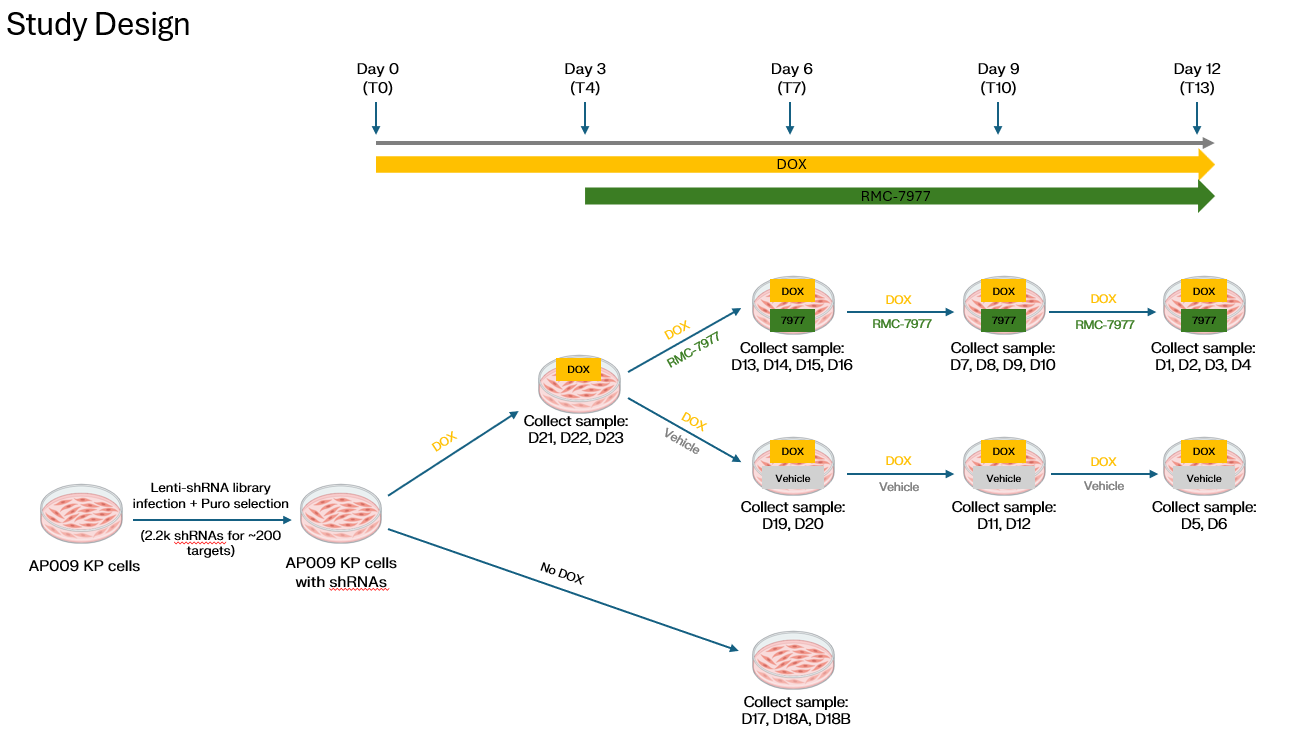
\includegraphics[keepaspectratio]{schematic_workflow_experimental_design.png}}
\caption{multiplexed shRNA screening experiment}
\end{figure}

    \begin{tcolorbox}[breakable, size=fbox, boxrule=1pt, pad at break*=1mm,colback=cellbackground, colframe=cellborder]
\prompt{In}{incolor}{6}{\boxspacing}
\begin{Verbatim}[commandchars=\\\{\}]
\PY{c+c1}{\PYZsh{} \PYZsh{}\PYZsh{}\PYZsh{}\PYZsh{} experimental design xlsx file}
\PY{c+c1}{\PYZsh{} file\PYZus{}path = \PYZdq{}\PYZti{}/Documents/Projects/Multi\PYZus{}shRNA\PYZus{}screening\PYZus{}AP009/data/Multiplexed shRNA screen in 2D AP009 \PYZhy{} Cellecta.xlsx\PYZdq{}}

\PY{c+c1}{\PYZsh{} xls = pd.ExcelFile(file\PYZus{}path)}

\PY{c+c1}{\PYZsh{} \PYZsh{}\PYZsh{} Gene targets}
\PY{c+c1}{\PYZsh{} gene\PYZus{}targets\PYZus{}df = pd.read\PYZus{}excel(xls, sheet\PYZus{}name=\PYZdq{}Master list\PYZdq{})}
\PY{c+c1}{\PYZsh{} \PYZsh{} Filter out \PYZdq{}Individual dual shRNA vector\PYZdq{} from gene targets}
\PY{c+c1}{\PYZsh{} filtered\PYZus{}gene\PYZus{}targets\PYZus{}df = gene\PYZus{}targets\PYZus{}df[gene\PYZus{}targets\PYZus{}df[\PYZdq{}Vector type\PYZdq{}] != \PYZdq{}Individual dual shRNA vector\PYZdq{}]}
\PY{c+c1}{\PYZsh{} filtered\PYZus{}gene\PYZus{}targets = filtered\PYZus{}gene\PYZus{}targets\PYZus{}df[\PYZdq{}Mouse gene symbol\PYZdq{}].dropna().unique()}

\PY{c+c1}{\PYZsh{} \PYZsh{} \PYZsh{}\PYZsh{} Define experimental parameters}
\PY{c+c1}{\PYZsh{} \PYZsh{} \PYZsh{} Num clonal barcodes per gene}
\PY{c+c1}{\PYZsh{} \PYZsh{} num\PYZus{}clonal\PYZus{}barcodes = 12000  }
\PY{c+c1}{\PYZsh{} \PYZsh{} \PYZsh{} Num shRNAs per gene}
\PY{c+c1}{\PYZsh{} \PYZsh{} num\PYZus{}shRNAs\PYZus{}per\PYZus{}gene = 10  }
\PY{c+c1}{\PYZsh{} \PYZsh{} \PYZsh{} N\PYZus{}reps per condition per timepoint}
\PY{c+c1}{\PYZsh{} \PYZsh{} num\PYZus{}replicates = 2  }

\PY{c+c1}{\PYZsh{} \PYZsh{}\PYZsh{} Define experimental conditions and timepoints }
\PY{c+c1}{\PYZsh{} \PYZsh{} available timepoints}
\PY{c+c1}{\PYZsh{} time\PYZus{}points = [\PYZdq{}0d\PYZdq{}, \PYZdq{}3d\PYZdq{}, \PYZdq{}6d\PYZdq{}, \PYZdq{}9d\PYZdq{}]}
\PY{c+c1}{\PYZsh{} \PYZsh{} experimental conditions based on design}
\PY{c+c1}{\PYZsh{} conditions = [}
\PY{c+c1}{\PYZsh{}     \PYZdq{}Baseline\PYZus{}NoDox\PYZus{}Vehicle\PYZdq{},}
\PY{c+c1}{\PYZsh{}     \PYZdq{}Baseline\PYZus{}Dox\PYZus{}PreTx\PYZdq{},  \PYZsh{} Only at 0d}
\PY{c+c1}{\PYZsh{}     \PYZdq{}Prognostic\PYZus{}Dox\PYZus{}Vehicle\PYZdq{},}
\PY{c+c1}{\PYZsh{}     \PYZdq{}Predictive\PYZus{}Dox\PYZus{}7977\PYZus{}LowDose\PYZdq{},  \PYZsh{} IC30 early, IC50 later}
\PY{c+c1}{\PYZsh{}     \PYZdq{}Predictive\PYZus{}Dox\PYZus{}7977\PYZus{}HighDose\PYZdq{}  \PYZsh{} IC90}
\PY{c+c1}{\PYZsh{} ]}
\end{Verbatim}
\end{tcolorbox}

    \begin{tcolorbox}[breakable, size=fbox, boxrule=1pt, pad at break*=1mm,colback=cellbackground, colframe=cellborder]
\prompt{In}{incolor}{298}{\boxspacing}
\begin{Verbatim}[commandchars=\\\{\}]
\PY{c+c1}{\PYZsh{}\PYZsh{}\PYZsh{}\PYZsh{} sample description xlsx file}
\PY{c+c1}{\PYZsh{} file\PYZus{}path\PYZus{}cellecta = \PYZdq{}\PYZti{}/Documents/Projects/Multi\PYZus{}shRNA\PYZus{}screening\PYZus{}AP009/data/sample\PYZus{}description\PYZus{}rectified.xlsx\PYZdq{}}
\PY{n}{file\PYZus{}path\PYZus{}cellecta} \PY{o}{=} \PY{n}{os}\PY{o}{.}\PY{n}{path}\PY{o}{.}\PY{n}{join}\PY{p}{(}\PY{n}{proj\PYZus{}dir}\PY{p}{,} \PY{l+s+s2}{\PYZdq{}}\PY{l+s+s2}{data/sample\PYZus{}description\PYZus{}rectified.xlsx}\PY{l+s+s2}{\PYZdq{}}\PY{p}{)}

\PY{n}{df\PYZus{}sd} \PY{o}{=} \PY{n}{pd}\PY{o}{.}\PY{n}{read\PYZus{}excel}\PY{p}{(}\PY{n}{file\PYZus{}path\PYZus{}cellecta}\PY{p}{,} \PY{n}{sheet\PYZus{}name}\PY{o}{=}\PY{l+s+s1}{\PYZsq{}}\PY{l+s+s1}{Sheet1}\PY{l+s+s1}{\PYZsq{}}\PY{p}{)}

\PY{c+c1}{\PYZsh{} Set the first row as column headers and remove it from the data}
\PY{n}{df\PYZus{}sd}\PY{o}{.}\PY{n}{columns} \PY{o}{=} \PY{n}{df\PYZus{}sd}\PY{o}{.}\PY{n}{iloc}\PY{p}{[}\PY{l+m+mi}{0}\PY{p}{]}
\PY{n}{df\PYZus{}sd} \PY{o}{=} \PY{n}{df\PYZus{}sd}\PY{p}{[}\PY{l+m+mi}{1}\PY{p}{:}\PY{p}{]}\PY{o}{.}\PY{n}{reset\PYZus{}index}\PY{p}{(}\PY{n}{drop}\PY{o}{=}\PY{k+kc}{True}\PY{p}{)}

\PY{c+c1}{\PYZsh{} Rename columns to remove any unintended whitespace}
\PY{n}{df\PYZus{}sd}\PY{o}{.}\PY{n}{columns} \PY{o}{=} \PY{n}{df\PYZus{}sd}\PY{o}{.}\PY{n}{columns}\PY{o}{.}\PY{n}{str}\PY{o}{.}\PY{n}{strip}\PY{p}{(}\PY{p}{)}
\end{Verbatim}
\end{tcolorbox}

    Utility function of table viewing

    \begin{tcolorbox}[breakable, size=fbox, boxrule=1pt, pad at break*=1mm,colback=cellbackground, colframe=cellborder]
\prompt{In}{incolor}{299}{\boxspacing}
\begin{Verbatim}[commandchars=\\\{\}]
\PY{n}{display}\PY{p}{(}\PY{n}{df\PYZus{}sd}\PY{p}{)}
\end{Verbatim}
\end{tcolorbox}

    
    \begin{Verbatim}[commandchars=\\\{\}]
0  Sample\_ID Sample\_Description         Library  \textbackslash{}
0         D1      T13\_Dox\_0.6nM  2.2K-REVMED-ZZ   
1         D2      T13\_Dox\_0.6nM  2.2K-REVMED-ZZ   
2         D3      T13\_Dox\_3.5nM  2.2K-REVMED-ZZ   
3         D4      T13\_Dox\_3.5nM  2.2K-REVMED-ZZ   
4         D5    T13\_Dox\_Vehicle  2.2K-REVMED-ZZ   
5         D6    T13\_Dox\_Vehicle  2.2K-REVMED-ZZ   
6         D7      T10\_Dox\_0.6nM  2.2K-REVMED-ZZ   
7         D8      T10\_Dox\_0.6nM  2.2K-REVMED-ZZ   
8         D9      T10\_Dox\_3.5nM  2.2K-REVMED-ZZ   
9        D10      T10\_Dox\_3.5nM  2.2K-REVMED-ZZ   
10       D11    T10\_Dox\_Vehicle  2.2K-REVMED-ZZ   
11       D12    T10\_Dox\_Vehicle  2.2K-REVMED-ZZ   
12       D13       T7\_Dox\_0.6nM  2.2K-REVMED-ZZ   
13       D14       T7\_Dox\_0.6nM  2.2K-REVMED-ZZ   
14       D15       T7\_Dox\_3.5nM  2.2K-REVMED-ZZ   
15       D16       T7\_Dox\_3.5nM  2.2K-REVMED-ZZ   
16       D17      T7\_NoDox\_NoTx  2.2K-REVMED-ZZ   
17     D18-A      T7\_NoDox\_NoTx  2.2K-REVMED-ZZ   
18     D18-B      T7\_NoDox\_NoTx  2.2K-REVMED-ZZ   
19       D19     T7\_Dox\_Vehicle  2.2K-REVMED-ZZ   
20       D20     T7\_Dox\_Vehicle  2.2K-REVMED-ZZ   
21       D21        T4\_Dox\_NoTx  2.2K-REVMED-ZZ   
22       D22        T4\_Dox\_NoTx  2.2K-REVMED-ZZ   
23       D23        T4\_Dox\_NoTx  2.2K-REVMED-ZZ   
24   plasmid            plasmid  2.2K-REVMED-ZZ   

0                                           Vector           Flowcell  \textbackslash{}
0    pRSIT16cb-U6tet-sh-CMV-tetR-2A-TagRFP-2A-Puro  25-03-11  102190    
1    pRSIT16cb-U6tet-sh-CMV-tetR-2A-TagRFP-2A-Puro  25-03-11  102190    
2    pRSIT16cb-U6tet-sh-CMV-tetR-2A-TagRFP-2A-Puro  25-03-11  102190    
3    pRSIT16cb-U6tet-sh-CMV-tetR-2A-TagRFP-2A-Puro  25-03-11  102190    
4    pRSIT16cb-U6tet-sh-CMV-tetR-2A-TagRFP-2A-Puro  25-03-11  102190    
5    pRSIT16cb-U6tet-sh-CMV-tetR-2A-TagRFP-2A-Puro  25-03-11  102190    
6    pRSIT16cb-U6tet-sh-CMV-tetR-2A-TagRFP-2A-Puro  25-03-11  102190    
7    pRSIT16cb-U6tet-sh-CMV-tetR-2A-TagRFP-2A-Puro  25-03-11  102190    
8    pRSIT16cb-U6tet-sh-CMV-tetR-2A-TagRFP-2A-Puro  25-03-11  102190    
9    pRSIT16cb-U6tet-sh-CMV-tetR-2A-TagRFP-2A-Puro  25-03-11  102190    
10   pRSIT16cb-U6tet-sh-CMV-tetR-2A-TagRFP-2A-Puro  25-03-11  102190    
11   pRSIT16cb-U6tet-sh-CMV-tetR-2A-TagRFP-2A-Puro  25-03-11  102190    
12   pRSIT16cb-U6tet-sh-CMV-tetR-2A-TagRFP-2A-Puro  25-03-11  102190    
13   pRSIT16cb-U6tet-sh-CMV-tetR-2A-TagRFP-2A-Puro  25-03-11  102190    
14   pRSIT16cb-U6tet-sh-CMV-tetR-2A-TagRFP-2A-Puro  25-03-11  102190    
15   pRSIT16cb-U6tet-sh-CMV-tetR-2A-TagRFP-2A-Puro  25-03-11  102190    
16   pRSIT16cb-U6tet-sh-CMV-tetR-2A-TagRFP-2A-Puro  25-03-11  102190    
17   pRSIT16cb-U6tet-sh-CMV-tetR-2A-TagRFP-2A-Puro  25-03-11  102190    
18   pRSIT16cb-U6tet-sh-CMV-tetR-2A-TagRFP-2A-Puro  25-03-11  102190    
19   pRSIT16cb-U6tet-sh-CMV-tetR-2A-TagRFP-2A-Puro  25-03-11  102190    
20   pRSIT16cb-U6tet-sh-CMV-tetR-2A-TagRFP-2A-Puro  25-03-11  102190    
21   pRSIT16cb-U6tet-sh-CMV-tetR-2A-TagRFP-2A-Puro  25-03-11  102190    
22   pRSIT16cb-U6tet-sh-CMV-tetR-2A-TagRFP-2A-Puro  25-03-11  102190    
23   pRSIT16cb-U6tet-sh-CMV-tetR-2A-TagRFP-2A-Puro  25-03-11  102190    
24   pRSIT16cb-U6tet-sh-CMV-tetR-2A-TagRFP-2A-Puro  25-03-11  102190    

0        Tx   Group Day\_Tx Replicate  Dox                            Note  
0       Low       5      9         2    Y                             NaN  
1       Low       5      9         1    Y                             NaN  
2      High       4      9         2    Y                             NaN  
3      High       4      9         1    Y                             NaN  
4   Vehicle       2      9         2    Y                             NaN  
5   Vehicle       2      9         1    Y                             NaN  
6       Low       5      6         2    Y                             NaN  
7       Low       5      6         1    Y                             NaN  
8      High       4      6         2    Y                             NaN  
9      High       4      6         1    Y                             NaN  
10  Vehicle       2      6         2    Y                             NaN  
11  Vehicle       2      6         1    Y                             NaN  
12      Low       5      3         2    Y                             NaN  
13      Low       5      3         1    Y                             NaN  
14     High       4      3         2    Y                             NaN  
15     High       4      3         1    Y                             NaN  
16     None       1      3         2    N                             NaN  
17     None       1      3         1    N                             NaN  
18     None       1      3         3    N  should tech rep be in group 2?  
19  Vehicle       2      3         2    Y                             NaN  
20  Vehicle       2      3         1    Y                             NaN  
21     None  pre-Tx      0         3    Y     should this be replicate 3?  
22     None  pre-Tx      0         2    Y                             NaN  
23     None  pre-Tx      0         1    Y                             NaN  
24      NaN     NaN    NaN       NaN  NaN                             NaN  
    \end{Verbatim}

    
    \subsection{Barcodes (shRNA) count
table}\label{barcodes-shrna-count-table}

Load count table (from Cellecta) and extract fields of sample IDs and
target gene

    \begin{tcolorbox}[breakable, size=fbox, boxrule=1pt, pad at break*=1mm,colback=cellbackground, colframe=cellborder]
\prompt{In}{incolor}{161}{\boxspacing}
\begin{Verbatim}[commandchars=\\\{\}]
\PY{c+c1}{\PYZsh{} file\PYZus{}path\PYZus{}count\PYZus{}table = \PYZdq{}\PYZti{}/Documents/Projects/Multi\PYZus{}shRNA\PYZus{}screening\PYZus{}AP009/data/Count\PYZus{}Table.csv\PYZdq{}}
\PY{n}{file\PYZus{}path\PYZus{}count\PYZus{}table} \PY{o}{=} \PY{n}{os}\PY{o}{.}\PY{n}{path}\PY{o}{.}\PY{n}{join}\PY{p}{(}\PY{n}{proj\PYZus{}dir}\PY{p}{,} \PY{l+s+s2}{\PYZdq{}}\PY{l+s+s2}{data/Count\PYZus{}Table.csv}\PY{l+s+s2}{\PYZdq{}}\PY{p}{)}

\PY{n}{df\PYZus{}counts} \PY{o}{=} \PY{n}{pd}\PY{o}{.}\PY{n}{read\PYZus{}csv}\PY{p}{(}\PY{n}{file\PYZus{}path\PYZus{}count\PYZus{}table}\PY{p}{)}

\PY{c+c1}{\PYZsh{} Extract columns that start with \PYZsq{}D\PYZsq{} plus the \PYZsq{}Gene Symbol / Target Name\PYZsq{} column}
\PY{n}{selected\PYZus{}columns} \PY{o}{=} \PY{p}{[}\PY{n}{col} \PY{k}{for} \PY{n}{col} \PY{o+ow}{in} \PY{n}{df\PYZus{}counts}\PY{o}{.}\PY{n}{columns} \PY{k}{if} \PY{n}{col}\PY{o}{.}\PY{n}{startswith}\PY{p}{(}\PY{l+s+s2}{\PYZdq{}}\PY{l+s+s2}{D}\PY{l+s+s2}{\PYZdq{}}\PY{p}{)}\PY{p}{]} \PY{o}{+} \PY{p}{[}\PY{l+s+s2}{\PYZdq{}}\PY{l+s+s2}{Gene Symbol / Target Name}\PY{l+s+s2}{\PYZdq{}}\PY{p}{,} \PY{l+s+s2}{\PYZdq{}}\PY{l+s+s2}{plasmid}\PY{l+s+s2}{\PYZdq{}}\PY{p}{]}

\PY{c+c1}{\PYZsh{} Create a new dataframe with selected columns}
\PY{n}{df\PYZus{}counts} \PY{o}{=} \PY{n}{df\PYZus{}counts}\PY{p}{[}\PY{n}{selected\PYZus{}columns}\PY{p}{]}\PY{o}{.}\PY{n}{copy}\PY{p}{(}\PY{p}{)}

\PY{c+c1}{\PYZsh{} Rename \PYZsq{}Gene Symbol / Target Name\PYZsq{} to \PYZsq{}target\PYZus{}gene\PYZsq{}}
\PY{n}{df\PYZus{}counts} \PY{o}{=} \PY{n}{df\PYZus{}counts}\PY{o}{.}\PY{n}{rename}\PY{p}{(}\PY{n}{columns}\PY{o}{=}\PY{p}{\PYZob{}}\PY{l+s+s2}{\PYZdq{}}\PY{l+s+s2}{Gene Symbol / Target Name}\PY{l+s+s2}{\PYZdq{}}\PY{p}{:} \PY{l+s+s2}{\PYZdq{}}\PY{l+s+s2}{Target\PYZus{}Gene}\PY{l+s+s2}{\PYZdq{}}\PY{p}{\PYZcb{}}\PY{p}{)}

\PY{c+c1}{\PYZsh{} Rename \PYZsq{}Non\PYZhy{}Targeting\PYZhy{}Mouse\PYZsq{} to \PYZsq{}NT\PYZsq{} in the target\PYZus{}gene column}
\PY{n}{df\PYZus{}counts}\PY{p}{[}\PY{l+s+s2}{\PYZdq{}}\PY{l+s+s2}{Target\PYZus{}Gene}\PY{l+s+s2}{\PYZdq{}}\PY{p}{]} \PY{o}{=} \PY{n}{df\PYZus{}counts}\PY{p}{[}\PY{l+s+s2}{\PYZdq{}}\PY{l+s+s2}{Target\PYZus{}Gene}\PY{l+s+s2}{\PYZdq{}}\PY{p}{]}\PY{o}{.}\PY{n}{replace}\PY{p}{(}\PY{l+s+s2}{\PYZdq{}}\PY{l+s+s2}{Non\PYZhy{}Targeting\PYZhy{}Mouse}\PY{l+s+s2}{\PYZdq{}}\PY{p}{,} \PY{l+s+s2}{\PYZdq{}}\PY{l+s+s2}{NT}\PY{l+s+s2}{\PYZdq{}}\PY{p}{)}

\PY{c+c1}{\PYZsh{} Ensure there are no NaN values in the target\PYZus{}gene column before counting repeats}
\PY{n}{df\PYZus{}counts}\PY{p}{[}\PY{l+s+s2}{\PYZdq{}}\PY{l+s+s2}{Target\PYZus{}Gene}\PY{l+s+s2}{\PYZdq{}}\PY{p}{]} \PY{o}{=} \PY{n}{df\PYZus{}counts}\PY{p}{[}\PY{l+s+s2}{\PYZdq{}}\PY{l+s+s2}{Target\PYZus{}Gene}\PY{l+s+s2}{\PYZdq{}}\PY{p}{]}\PY{o}{.}\PY{n}{fillna}\PY{p}{(}\PY{l+s+s2}{\PYZdq{}}\PY{l+s+s2}{Unknown}\PY{l+s+s2}{\PYZdq{}}\PY{p}{)}

\PY{c+c1}{\PYZsh{} Generate a sequential ID for each occurrence of target\PYZus{}gene}
\PY{n}{df\PYZus{}counts}\PY{p}{[}\PY{l+s+s2}{\PYZdq{}}\PY{l+s+s2}{target\PYZus{}gene\PYZus{}repeat\PYZus{}ID}\PY{l+s+s2}{\PYZdq{}}\PY{p}{]} \PY{o}{=} \PY{n}{df\PYZus{}counts}\PY{o}{.}\PY{n}{groupby}\PY{p}{(}\PY{l+s+s2}{\PYZdq{}}\PY{l+s+s2}{Target\PYZus{}Gene}\PY{l+s+s2}{\PYZdq{}}\PY{p}{)}\PY{o}{.}\PY{n}{cumcount}\PY{p}{(}\PY{p}{)} \PY{o}{+} \PY{l+m+mi}{1}

\PY{c+c1}{\PYZsh{} Format as \PYZdq{}01\PYZdq{}, \PYZdq{}02\PYZdq{}, \PYZdq{}03\PYZdq{}, etc.}
\PY{n}{df\PYZus{}counts}\PY{p}{[}\PY{l+s+s2}{\PYZdq{}}\PY{l+s+s2}{target\PYZus{}gene\PYZus{}repeat\PYZus{}ID}\PY{l+s+s2}{\PYZdq{}}\PY{p}{]} \PY{o}{=} \PY{n}{df\PYZus{}counts}\PY{p}{[}\PY{l+s+s2}{\PYZdq{}}\PY{l+s+s2}{target\PYZus{}gene\PYZus{}repeat\PYZus{}ID}\PY{l+s+s2}{\PYZdq{}}\PY{p}{]}\PY{o}{.}\PY{n}{astype}\PY{p}{(}\PY{n+nb}{int}\PY{p}{)}\PY{o}{.}\PY{n}{apply}\PY{p}{(}\PY{k}{lambda} \PY{n}{x}\PY{p}{:} \PY{l+s+sa}{f}\PY{l+s+s2}{\PYZdq{}}\PY{l+s+si}{\PYZob{}}\PY{n}{x}\PY{l+s+si}{:}\PY{l+s+s2}{02d}\PY{l+s+si}{\PYZcb{}}\PY{l+s+s2}{\PYZdq{}}\PY{p}{)}

\PY{c+c1}{\PYZsh{} Combine with target\PYZus{}gene to create a unique ID}
\PY{n}{df\PYZus{}counts}\PY{p}{[}\PY{l+s+s2}{\PYZdq{}}\PY{l+s+s2}{shRNA\PYZus{}ID}\PY{l+s+s2}{\PYZdq{}}\PY{p}{]} \PY{o}{=} \PY{n}{df\PYZus{}counts}\PY{p}{[}\PY{l+s+s2}{\PYZdq{}}\PY{l+s+s2}{Target\PYZus{}Gene}\PY{l+s+s2}{\PYZdq{}}\PY{p}{]} \PY{o}{+} \PY{l+s+s2}{\PYZdq{}}\PY{l+s+s2}{\PYZus{}}\PY{l+s+s2}{\PYZdq{}} \PY{o}{+} \PY{n}{df\PYZus{}counts}\PY{p}{[}\PY{l+s+s2}{\PYZdq{}}\PY{l+s+s2}{target\PYZus{}gene\PYZus{}repeat\PYZus{}ID}\PY{l+s+s2}{\PYZdq{}}\PY{p}{]}

\PY{c+c1}{\PYZsh{} Drop the temporary repeat ID column}
\PY{n}{df\PYZus{}counts} \PY{o}{=} \PY{n}{df\PYZus{}counts}\PY{o}{.}\PY{n}{drop}\PY{p}{(}\PY{n}{columns}\PY{o}{=}\PY{p}{[}\PY{l+s+s2}{\PYZdq{}}\PY{l+s+s2}{target\PYZus{}gene\PYZus{}repeat\PYZus{}ID}\PY{l+s+s2}{\PYZdq{}}\PY{p}{]}\PY{p}{)}

\PY{c+c1}{\PYZsh{} Update the target\PYZus{}gene\PYZus{}ID column accordingly}
\PY{n}{df\PYZus{}counts}\PY{p}{[}\PY{l+s+s2}{\PYZdq{}}\PY{l+s+s2}{shRNA\PYZus{}ID}\PY{l+s+s2}{\PYZdq{}}\PY{p}{]} \PY{o}{=} \PY{n}{df\PYZus{}counts}\PY{p}{[}\PY{l+s+s2}{\PYZdq{}}\PY{l+s+s2}{Target\PYZus{}Gene}\PY{l+s+s2}{\PYZdq{}}\PY{p}{]} \PY{o}{+} \PY{l+s+s2}{\PYZdq{}}\PY{l+s+s2}{\PYZus{}}\PY{l+s+s2}{\PYZdq{}} \PY{o}{+} \PY{n}{df\PYZus{}counts}\PY{p}{[}\PY{l+s+s2}{\PYZdq{}}\PY{l+s+s2}{shRNA\PYZus{}ID}\PY{l+s+s2}{\PYZdq{}}\PY{p}{]}\PY{o}{.}\PY{n}{str}\PY{o}{.}\PY{n}{split}\PY{p}{(}\PY{l+s+s2}{\PYZdq{}}\PY{l+s+s2}{\PYZus{}}\PY{l+s+s2}{\PYZdq{}}\PY{p}{)}\PY{o}{.}\PY{n}{str}\PY{p}{[}\PY{o}{\PYZhy{}}\PY{l+m+mi}{1}\PY{p}{]}

\PY{c+c1}{\PYZsh{} melt the dataframe to long format }
\PY{n}{df\PYZus{}long} \PY{o}{=} \PY{n}{df\PYZus{}counts}\PY{o}{.}\PY{n}{melt}\PY{p}{(}\PY{n}{id\PYZus{}vars}\PY{o}{=}\PY{p}{[}\PY{l+s+s2}{\PYZdq{}}\PY{l+s+s2}{Target\PYZus{}Gene}\PY{l+s+s2}{\PYZdq{}}\PY{p}{,} \PY{l+s+s2}{\PYZdq{}}\PY{l+s+s2}{shRNA\PYZus{}ID}\PY{l+s+s2}{\PYZdq{}}\PY{p}{]}\PY{p}{,} \PY{n}{var\PYZus{}name}\PY{o}{=}\PY{l+s+s2}{\PYZdq{}}\PY{l+s+s2}{Sample\PYZus{}ID}\PY{l+s+s2}{\PYZdq{}}\PY{p}{,} \PY{n}{value\PYZus{}name}\PY{o}{=}\PY{l+s+s2}{\PYZdq{}}\PY{l+s+s2}{Read\PYZus{}Counts}\PY{l+s+s2}{\PYZdq{}}\PY{p}{)}
\end{Verbatim}
\end{tcolorbox}

    \begin{tcolorbox}[breakable, size=fbox, boxrule=1pt, pad at break*=1mm,colback=cellbackground, colframe=cellborder]
\prompt{In}{incolor}{162}{\boxspacing}
\begin{Verbatim}[commandchars=\\\{\}]
\PY{n}{display}\PY{p}{(}\PY{n}{df\PYZus{}counts}\PY{p}{)}
\end{Verbatim}
\end{tcolorbox}

    
    \begin{Verbatim}[commandchars=\\\{\}]
        D1    D2    D3    D4    D5    D6    D7    D8    D9   D10  {\ldots}  D18-A  \textbackslash{}
0     1399  2777  1312  2281  2056  1579  1072  3116  2532  3019  {\ldots}   1411   
1     1785  3277  1776  3414  3139  2482  1289  3877  3373  3953  {\ldots}   2000   
2      569  1270   539  1025  1075   892   484  1728  1201  1301  {\ldots}    726   
3      955  1703   912  1607  1714  1235   817  2199  1727  2160  {\ldots}   1153   
4     1150  2403  1177  2281  1981  1467  1055  2641  2071  2504  {\ldots}   1415   
{\ldots}    {\ldots}   {\ldots}   {\ldots}   {\ldots}   {\ldots}   {\ldots}   {\ldots}   {\ldots}   {\ldots}   {\ldots}  {\ldots}    {\ldots}   
2182   460   889   548   870   810   571   332  1141   935  1101  {\ldots}    679   
2183   725  1451   709  1416  1151  1017   483  1693  1601  1726  {\ldots}    782   
2184   547  1133   575  1052  1093   843   477  1365  1246  1497  {\ldots}    771   
2185  1354  2584  1371  2570  2230  1773  1047  3223  2530  3248  {\ldots}   1610   
2186   479   960   497   907   832   562   368  1276   813  1025  {\ldots}    534   

      D18-B   D19   D20   D21   D22   D23  Target\_Gene  plasmid  shRNA\_ID  
0      1717  1682  2105  1482  1257  1965           NT     3776     NT\_01  
1      2510  2559  2959  2321  1782  2763           NT     4949     NT\_02  
2       804   774  1094   768   601   945           NT     1881     NT\_03  
3      1372  1268  1481  1010   855  1385           NT     2748     NT\_04  
4      1599  1556  2025  1541  1126  1868           NT     3560     NT\_05  
{\ldots}     {\ldots}   {\ldots}   {\ldots}   {\ldots}   {\ldots}   {\ldots}          {\ldots}      {\ldots}       {\ldots}  
2182    758   709   892   658   475   859         Zeb1     1552   Zeb1\_06  
2183    970   933  1242   931   757  1071         Zeb1     2043   Zeb1\_07  
2184    868   820  1157   698   637   846         Zeb1     2101   Zeb1\_08  
2185   1877  1745  2160  1681  1329  1973         Zeb1     4534   Zeb1\_09  
2186    597   583   787   609   474   691         Zeb1     1383   Zeb1\_10  

[2187 rows x 27 columns]
    \end{Verbatim}

    
    \begin{tcolorbox}[breakable, size=fbox, boxrule=1pt, pad at break*=1mm,colback=cellbackground, colframe=cellborder]
\prompt{In}{incolor}{163}{\boxspacing}
\begin{Verbatim}[commandchars=\\\{\}]
\PY{n}{display}\PY{p}{(}\PY{n}{df\PYZus{}long}\PY{p}{)}
\end{Verbatim}
\end{tcolorbox}

    
    \begin{Verbatim}[commandchars=\\\{\}]
      Target\_Gene shRNA\_ID Sample\_ID  Read\_Counts
0              NT    NT\_01        D1         1399
1              NT    NT\_02        D1         1785
2              NT    NT\_03        D1          569
3              NT    NT\_04        D1          955
4              NT    NT\_05        D1         1150
{\ldots}           {\ldots}      {\ldots}       {\ldots}          {\ldots}
54670        Zeb1  Zeb1\_06   plasmid         1552
54671        Zeb1  Zeb1\_07   plasmid         2043
54672        Zeb1  Zeb1\_08   plasmid         2101
54673        Zeb1  Zeb1\_09   plasmid         4534
54674        Zeb1  Zeb1\_10   plasmid         1383

[54675 rows x 4 columns]
    \end{Verbatim}

    
    \subsubsection{Total number of barcodes per sample /
condition}\label{total-number-of-barcodes-per-sample-condition}

    \begin{tcolorbox}[breakable, size=fbox, boxrule=1pt, pad at break*=1mm,colback=cellbackground, colframe=cellborder]
\prompt{In}{incolor}{165}{\boxspacing}
\begin{Verbatim}[commandchars=\\\{\}]
\PY{n}{df\PYZus{}full} \PY{o}{=} \PY{n}{df\PYZus{}long}\PY{o}{.}\PY{n}{merge}\PY{p}{(}\PY{n}{df\PYZus{}sd}\PY{p}{[}\PY{p}{[}\PY{l+s+s2}{\PYZdq{}}\PY{l+s+s2}{Sample\PYZus{}ID}\PY{l+s+s2}{\PYZdq{}}\PY{p}{,} \PY{l+s+s2}{\PYZdq{}}\PY{l+s+s2}{Sample\PYZus{}Description}\PY{l+s+s2}{\PYZdq{}}\PY{p}{,} \PY{l+s+s2}{\PYZdq{}}\PY{l+s+s2}{Day\PYZus{}Tx}\PY{l+s+s2}{\PYZdq{}}\PY{p}{,} \PY{l+s+s2}{\PYZdq{}}\PY{l+s+s2}{Tx}\PY{l+s+s2}{\PYZdq{}}\PY{p}{,} \PY{l+s+s2}{\PYZdq{}}\PY{l+s+s2}{Dox}\PY{l+s+s2}{\PYZdq{}}\PY{p}{,} \PY{l+s+s2}{\PYZdq{}}\PY{l+s+s2}{Replicate}\PY{l+s+s2}{\PYZdq{}}\PY{p}{]}\PY{p}{]}\PY{p}{,} 
                        \PY{n}{left\PYZus{}on} \PY{o}{=} \PY{l+s+s2}{\PYZdq{}}\PY{l+s+s2}{Sample\PYZus{}ID}\PY{l+s+s2}{\PYZdq{}}\PY{p}{,} \PY{n}{right\PYZus{}on} \PY{o}{=} \PY{l+s+s2}{\PYZdq{}}\PY{l+s+s2}{Sample\PYZus{}ID}\PY{l+s+s2}{\PYZdq{}}\PY{p}{,} \PY{n}{how} \PY{o}{=} \PY{l+s+s2}{\PYZdq{}}\PY{l+s+s2}{left}\PY{l+s+s2}{\PYZdq{}}\PY{p}{)}
\PY{c+c1}{\PYZsh{} df\PYZus{}full.to\PYZus{}csv(\PYZdq{}\PYZti{}/Documents/Projects/Multi\PYZus{}shRNA\PYZus{}screening\PYZus{}AP009/data/long\PYZus{}format\PYZus{}joint\PYZus{}count\PYZus{}data.csv\PYZdq{}, index = False)}
\PY{n}{df\PYZus{}full}\PY{o}{.}\PY{n}{to\PYZus{}csv}\PY{p}{(}\PY{n}{os}\PY{o}{.}\PY{n}{path}\PY{o}{.}\PY{n}{join}\PY{p}{(}\PY{n}{proj\PYZus{}dir}\PY{p}{,} \PY{l+s+s2}{\PYZdq{}}\PY{l+s+s2}{data/long\PYZus{}format\PYZus{}joint\PYZus{}count\PYZus{}data.csv}\PY{l+s+s2}{\PYZdq{}}\PY{p}{)}\PY{p}{,} \PY{n}{index} \PY{o}{=} \PY{k+kc}{False}\PY{p}{)}
\end{Verbatim}
\end{tcolorbox}

    \begin{tcolorbox}[breakable, size=fbox, boxrule=1pt, pad at break*=1mm,colback=cellbackground, colframe=cellborder]
\prompt{In}{incolor}{166}{\boxspacing}
\begin{Verbatim}[commandchars=\\\{\}]
\PY{n}{display}\PY{p}{(}\PY{n}{df\PYZus{}full}\PY{p}{)}
\PY{n+nb}{print}\PY{p}{(}\PY{n}{df\PYZus{}full}\PY{p}{[}\PY{l+s+s2}{\PYZdq{}}\PY{l+s+s2}{Target\PYZus{}Gene}\PY{l+s+s2}{\PYZdq{}}\PY{p}{]}\PY{o}{.}\PY{n}{value\PYZus{}counts}\PY{p}{(}\PY{p}{)}\PY{p}{)}
\PY{n+nb}{print}\PY{p}{(}\PY{n}{df\PYZus{}full}\PY{p}{[}\PY{l+s+s2}{\PYZdq{}}\PY{l+s+s2}{Sample\PYZus{}Description}\PY{l+s+s2}{\PYZdq{}}\PY{p}{]}\PY{o}{.}\PY{n}{value\PYZus{}counts}\PY{p}{(}\PY{p}{)}\PY{p}{)}
\end{Verbatim}
\end{tcolorbox}

    
    \begin{Verbatim}[commandchars=\\\{\}]
      Target\_Gene shRNA\_ID Sample\_ID  Read\_Counts Sample\_Description Day\_Tx  \textbackslash{}
0              NT    NT\_01        D1         1399      T13\_Dox\_0.6nM      9   
1              NT    NT\_02        D1         1785      T13\_Dox\_0.6nM      9   
2              NT    NT\_03        D1          569      T13\_Dox\_0.6nM      9   
3              NT    NT\_04        D1          955      T13\_Dox\_0.6nM      9   
4              NT    NT\_05        D1         1150      T13\_Dox\_0.6nM      9   
{\ldots}           {\ldots}      {\ldots}       {\ldots}          {\ldots}                {\ldots}    {\ldots}   
54670        Zeb1  Zeb1\_06   plasmid         1552            plasmid    NaN   
54671        Zeb1  Zeb1\_07   plasmid         2043            plasmid    NaN   
54672        Zeb1  Zeb1\_08   plasmid         2101            plasmid    NaN   
54673        Zeb1  Zeb1\_09   plasmid         4534            plasmid    NaN   
54674        Zeb1  Zeb1\_10   plasmid         1383            plasmid    NaN   

        Tx  Dox Replicate  
0      Low    Y         2  
1      Low    Y         2  
2      Low    Y         2  
3      Low    Y         2  
4      Low    Y         2  
{\ldots}    {\ldots}  {\ldots}       {\ldots}  
54670  NaN  NaN       NaN  
54671  NaN  NaN       NaN  
54672  NaN  NaN       NaN  
54673  NaN  NaN       NaN  
54674  NaN  NaN       NaN  

[54675 rows x 9 columns]
    \end{Verbatim}

    
    \begin{Verbatim}[commandchars=\\\{\}]
NT               5000
Pdgfra            250
Nf1               250
Nf2               250
Nfe2l2            250
                 {\ldots}
Erbb2             250
Erbb3             250
Ern1              250
Zeb1              250
Cdkn2a(Ink4a)     175
Name: Target\_Gene, Length: 200, dtype: int64
T7\_NoDox\_NoTx      6561
T4\_Dox\_NoTx        6561
T13\_Dox\_0.6nM      4374
T13\_Dox\_3.5nM      4374
T13\_Dox\_Vehicle    4374
T10\_Dox\_0.6nM      4374
T10\_Dox\_3.5nM      4374
T10\_Dox\_Vehicle    4374
T7\_Dox\_0.6nM       4374
T7\_Dox\_3.5nM       4374
T7\_Dox\_Vehicle     4374
plasmid            2187
Name: Sample\_Description, dtype: int64
    \end{Verbatim}

    \subsubsection{Count correlation between T7\_NoDox\_NoTx (D17, D18-A,
D18-B) and
plasmid}\label{count-correlation-between-t7_nodox_notx-d17-d18-a-d18-b-and-plasmid}

    \begin{tcolorbox}[breakable, size=fbox, boxrule=1pt, pad at break*=1mm,colback=cellbackground, colframe=cellborder]
\prompt{In}{incolor}{178}{\boxspacing}
\begin{Verbatim}[commandchars=\\\{\}]
\PY{n}{df\PYZus{}full} \PY{o}{=} \PY{n}{pd}\PY{o}{.}\PY{n}{read\PYZus{}csv}\PY{p}{(}\PY{n}{os}\PY{o}{.}\PY{n}{path}\PY{o}{.}\PY{n}{join}\PY{p}{(}\PY{n}{proj\PYZus{}dir}\PY{p}{,} \PY{l+s+s2}{\PYZdq{}}\PY{l+s+s2}{data/long\PYZus{}format\PYZus{}joint\PYZus{}count\PYZus{}data.csv}\PY{l+s+s2}{\PYZdq{}}\PY{p}{)}\PY{p}{)}

\PY{c+c1}{\PYZsh{} Pivot the data to wide format for pairwise comparisons using correct column name}
\PY{n}{df\PYZus{}pivot} \PY{o}{=} \PY{n}{df\PYZus{}full}\PY{o}{.}\PY{n}{pivot\PYZus{}table}\PY{p}{(}\PY{n}{index}\PY{o}{=}\PY{l+s+s2}{\PYZdq{}}\PY{l+s+s2}{shRNA\PYZus{}ID}\PY{l+s+s2}{\PYZdq{}}\PY{p}{,} \PY{n}{columns}\PY{o}{=}\PY{l+s+s2}{\PYZdq{}}\PY{l+s+s2}{Sample\PYZus{}ID}\PY{l+s+s2}{\PYZdq{}}\PY{p}{,} \PY{n}{values}\PY{o}{=}\PY{l+s+s2}{\PYZdq{}}\PY{l+s+s2}{Read\PYZus{}Counts}\PY{l+s+s2}{\PYZdq{}}\PY{p}{,} \PY{n}{aggfunc}\PY{o}{=}\PY{l+s+s2}{\PYZdq{}}\PY{l+s+s2}{sum}\PY{l+s+s2}{\PYZdq{}}\PY{p}{)}

\PY{c+c1}{\PYZsh{} Select the sample IDs of interest}
\PY{n}{sample\PYZus{}ids} \PY{o}{=} \PY{p}{[}\PY{l+s+s2}{\PYZdq{}}\PY{l+s+s2}{D17}\PY{l+s+s2}{\PYZdq{}}\PY{p}{,} \PY{l+s+s2}{\PYZdq{}}\PY{l+s+s2}{D18\PYZhy{}A}\PY{l+s+s2}{\PYZdq{}}\PY{p}{,} \PY{l+s+s2}{\PYZdq{}}\PY{l+s+s2}{D18\PYZhy{}B}\PY{l+s+s2}{\PYZdq{}}\PY{p}{,} \PY{l+s+s2}{\PYZdq{}}\PY{l+s+s2}{plasmid}\PY{l+s+s2}{\PYZdq{}}\PY{p}{]}

\PY{c+c1}{\PYZsh{} Keep only the relevant columns and drop any missing data}
\PY{n}{df\PYZus{}selected} \PY{o}{=} \PY{n}{df\PYZus{}pivot}\PY{p}{[}\PY{n}{sample\PYZus{}ids}\PY{p}{]}\PY{o}{.}\PY{n}{dropna}\PY{p}{(}\PY{p}{)}

\PY{k}{def} \PY{n+nf}{corrfunc}\PY{p}{(}\PY{n}{x}\PY{p}{,} \PY{n}{y}\PY{p}{,} \PY{o}{*}\PY{o}{*}\PY{n}{kws}\PY{p}{)}\PY{p}{:}
    \PY{n}{r} \PY{o}{=} \PY{n}{np}\PY{o}{.}\PY{n}{corrcoef}\PY{p}{(}\PY{n}{x}\PY{p}{,} \PY{n}{y}\PY{p}{)}\PY{p}{[}\PY{l+m+mi}{0}\PY{p}{,} \PY{l+m+mi}{1}\PY{p}{]}
    \PY{n}{ax} \PY{o}{=} \PY{n}{plt}\PY{o}{.}\PY{n}{gca}\PY{p}{(}\PY{p}{)}
    \PY{n}{ax}\PY{o}{.}\PY{n}{annotate}\PY{p}{(}\PY{l+s+sa}{f}\PY{l+s+s2}{\PYZdq{}}\PY{l+s+s2}{R = }\PY{l+s+si}{\PYZob{}}\PY{n}{r}\PY{l+s+si}{:}\PY{l+s+s2}{.2f}\PY{l+s+si}{\PYZcb{}}\PY{l+s+s2}{\PYZdq{}}\PY{p}{,} \PY{n}{xy}\PY{o}{=}\PY{p}{(}\PY{l+m+mf}{0.2}\PY{p}{,} \PY{l+m+mf}{0.5}\PY{p}{)}\PY{p}{,} \PY{n}{xycoords}\PY{o}{=}\PY{n}{ax}\PY{o}{.}\PY{n}{transAxes}\PY{p}{,} \PY{n}{fontsize}\PY{o}{=}\PY{l+m+mi}{25}\PY{p}{)}

\PY{n}{sns}\PY{o}{.}\PY{n}{set}\PY{p}{(}\PY{n}{style}\PY{o}{=}\PY{l+s+s2}{\PYZdq{}}\PY{l+s+s2}{whitegrid}\PY{l+s+s2}{\PYZdq{}}\PY{p}{)}
\PY{n}{g} \PY{o}{=} \PY{n}{sns}\PY{o}{.}\PY{n}{PairGrid}\PY{p}{(}\PY{n}{df\PYZus{}selected}\PY{p}{)}
\PY{n}{g}\PY{o}{.}\PY{n}{map\PYZus{}lower}\PY{p}{(}\PY{n}{sns}\PY{o}{.}\PY{n}{regplot}\PY{p}{,} \PY{n}{scatter\PYZus{}kws}\PY{o}{=}\PY{p}{\PYZob{}}\PY{l+s+s1}{\PYZsq{}}\PY{l+s+s1}{s}\PY{l+s+s1}{\PYZsq{}}\PY{p}{:} \PY{l+m+mi}{10}\PY{p}{,} \PY{l+s+s1}{\PYZsq{}}\PY{l+s+s1}{alpha}\PY{l+s+s1}{\PYZsq{}}\PY{p}{:} \PY{l+m+mf}{0.6}\PY{p}{\PYZcb{}}\PY{p}{,} \PY{n}{line\PYZus{}kws}\PY{o}{=}\PY{p}{\PYZob{}}\PY{l+s+s2}{\PYZdq{}}\PY{l+s+s2}{color}\PY{l+s+s2}{\PYZdq{}}\PY{p}{:} \PY{l+s+s2}{\PYZdq{}}\PY{l+s+s2}{red}\PY{l+s+s2}{\PYZdq{}}\PY{p}{\PYZcb{}}\PY{p}{)}
\PY{n}{g}\PY{o}{.}\PY{n}{map\PYZus{}diag}\PY{p}{(}\PY{n}{sns}\PY{o}{.}\PY{n}{histplot}\PY{p}{,} \PY{n}{bins}\PY{o}{=}\PY{l+m+mi}{30}\PY{p}{,} \PY{n}{kde}\PY{o}{=}\PY{k+kc}{True}\PY{p}{)}
\PY{n}{g}\PY{o}{.}\PY{n}{map\PYZus{}upper}\PY{p}{(}\PY{n}{corrfunc}\PY{p}{)}

\PY{k}{for} \PY{n}{i} \PY{o+ow}{in} \PY{n+nb}{range}\PY{p}{(}\PY{n+nb}{len}\PY{p}{(}\PY{n}{sample\PYZus{}ids}\PY{p}{)}\PY{p}{)}\PY{p}{:}
    \PY{k}{for} \PY{n}{j} \PY{o+ow}{in} \PY{n+nb}{range}\PY{p}{(}\PY{n+nb}{len}\PY{p}{(}\PY{n}{sample\PYZus{}ids}\PY{p}{)}\PY{p}{)}\PY{p}{:}
        \PY{n}{ax} \PY{o}{=} \PY{n}{g}\PY{o}{.}\PY{n}{axes}\PY{p}{[}\PY{n}{i}\PY{p}{,} \PY{n}{j}\PY{p}{]}
        \PY{k}{if} \PY{n}{ax} \PY{o+ow}{is} \PY{o+ow}{not} \PY{k+kc}{None}\PY{p}{:}
            \PY{n}{ax}\PY{o}{.}\PY{n}{set\PYZus{}xlim}\PY{p}{(}\PY{n}{left}\PY{o}{=}\PY{l+m+mi}{0}\PY{p}{)}
            \PY{n}{ax}\PY{o}{.}\PY{n}{set\PYZus{}ylim}\PY{p}{(}\PY{n}{bottom}\PY{o}{=}\PY{l+m+mi}{0}\PY{p}{)}

\PY{n}{plt}\PY{o}{.}\PY{n}{suptitle}\PY{p}{(}\PY{l+s+s2}{\PYZdq{}}\PY{l+s+s2}{Pairwise Scatterplots of Read Counts}\PY{l+s+s2}{\PYZdq{}}\PY{p}{,} \PY{n}{y}\PY{o}{=}\PY{l+m+mf}{1.02}\PY{p}{)}

\PY{c+c1}{\PYZsh{} Show the plot}
\PY{n}{plt}\PY{o}{.}\PY{n}{show}\PY{p}{(}\PY{p}{)}
\end{Verbatim}
\end{tcolorbox}

    \begin{center}
    \adjustimage{max size={0.9\linewidth}{0.9\paperheight}}{multi_shrna_screening_ap009_files/multi_shrna_screening_ap009_20_0.png}
    \end{center}
    { \hspace*{\fill} \\}
    
    \subsubsection{Total read counts per
sample}\label{total-read-counts-per-sample}

    \begin{tcolorbox}[breakable, size=fbox, boxrule=1pt, pad at break*=1mm,colback=cellbackground, colframe=cellborder]
\prompt{In}{incolor}{179}{\boxspacing}
\begin{Verbatim}[commandchars=\\\{\}]
\PY{n}{df\PYZus{}full} \PY{o}{=} \PY{n}{pd}\PY{o}{.}\PY{n}{read\PYZus{}csv}\PY{p}{(}\PY{n}{os}\PY{o}{.}\PY{n}{path}\PY{o}{.}\PY{n}{join}\PY{p}{(}\PY{n}{proj\PYZus{}dir}\PY{p}{,} \PY{l+s+s2}{\PYZdq{}}\PY{l+s+s2}{data/long\PYZus{}format\PYZus{}joint\PYZus{}count\PYZus{}data.csv}\PY{l+s+s2}{\PYZdq{}}\PY{p}{)}\PY{p}{)}

\PY{n}{df\PYZus{}counts} \PY{o}{=} \PY{n}{df\PYZus{}full}\PY{p}{[}\PY{n}{df\PYZus{}full}\PY{p}{[}\PY{l+s+s2}{\PYZdq{}}\PY{l+s+s2}{Sample\PYZus{}ID}\PY{l+s+s2}{\PYZdq{}}\PY{p}{]} \PY{o}{!=} \PY{l+s+s2}{\PYZdq{}}\PY{l+s+s2}{plasmid}\PY{l+s+s2}{\PYZdq{}}\PY{p}{]}

\PY{c+c1}{\PYZsh{} Aggregate total read counts per sample}
\PY{n}{df\PYZus{}sample\PYZus{}counts\PYZus{}simple} \PY{o}{=} \PY{n}{df\PYZus{}counts}\PY{o}{.}\PY{n}{groupby}\PY{p}{(}\PY{p}{[}\PY{l+s+s2}{\PYZdq{}}\PY{l+s+s2}{Sample\PYZus{}ID}\PY{l+s+s2}{\PYZdq{}}\PY{p}{,} \PY{l+s+s2}{\PYZdq{}}\PY{l+s+s2}{Sample\PYZus{}Description}\PY{l+s+s2}{\PYZdq{}}\PY{p}{]}\PY{p}{)}\PY{p}{[}\PY{l+s+s2}{\PYZdq{}}\PY{l+s+s2}{Read\PYZus{}Counts}\PY{l+s+s2}{\PYZdq{}}\PY{p}{]}\PY{o}{.}\PY{n}{sum}\PY{p}{(}\PY{p}{)}\PY{o}{.}\PY{n}{reset\PYZus{}index}\PY{p}{(}\PY{p}{)}

\PY{c+c1}{\PYZsh{} Ensure Sample\PYZus{}ID is sorted numerically rather than lexicographically}
\PY{n}{df\PYZus{}sample\PYZus{}counts\PYZus{}simple}\PY{p}{[}\PY{l+s+s2}{\PYZdq{}}\PY{l+s+s2}{Sample\PYZus{}ID\PYZus{}Sort}\PY{l+s+s2}{\PYZdq{}}\PY{p}{]} \PY{o}{=} \PY{n}{df\PYZus{}sample\PYZus{}counts\PYZus{}simple}\PY{p}{[}\PY{l+s+s2}{\PYZdq{}}\PY{l+s+s2}{Sample\PYZus{}ID}\PY{l+s+s2}{\PYZdq{}}\PY{p}{]}\PY{o}{.}\PY{n}{str}\PY{o}{.}\PY{n}{extract}\PY{p}{(}\PY{l+s+s1}{\PYZsq{}}\PY{l+s+s1}{(}\PY{l+s+s1}{\PYZbs{}}\PY{l+s+s1}{d+)}\PY{l+s+s1}{\PYZsq{}}\PY{p}{)}\PY{o}{.}\PY{n}{astype}\PY{p}{(}\PY{n+nb}{int}\PY{p}{)}
\PY{n}{df\PYZus{}sample\PYZus{}counts\PYZus{}simple} \PY{o}{=} \PY{n}{df\PYZus{}sample\PYZus{}counts\PYZus{}simple}\PY{o}{.}\PY{n}{sort\PYZus{}values}\PY{p}{(}\PY{n}{by}\PY{o}{=}\PY{l+s+s2}{\PYZdq{}}\PY{l+s+s2}{Sample\PYZus{}ID\PYZus{}Sort}\PY{l+s+s2}{\PYZdq{}}\PY{p}{)}\PY{o}{.}\PY{n}{reset\PYZus{}index}\PY{p}{(}\PY{p}{)}

\PY{c+c1}{\PYZsh{} Modify Sample\PYZus{}ID labels to include total counts in parentheses}
\PY{n}{df\PYZus{}sample\PYZus{}counts\PYZus{}simple}\PY{p}{[}\PY{l+s+s2}{\PYZdq{}}\PY{l+s+s2}{Sample\PYZus{}ID\PYZus{}Label}\PY{l+s+s2}{\PYZdq{}}\PY{p}{]} \PY{o}{=} \PY{n}{df\PYZus{}sample\PYZus{}counts\PYZus{}simple}\PY{o}{.}\PY{n}{apply}\PY{p}{(}
    \PY{k}{lambda} \PY{n}{row}\PY{p}{:} \PY{l+s+sa}{f}\PY{l+s+s2}{\PYZdq{}}\PY{l+s+si}{\PYZob{}}\PY{n}{row}\PY{p}{[}\PY{l+s+s1}{\PYZsq{}}\PY{l+s+s1}{Sample\PYZus{}ID}\PY{l+s+s1}{\PYZsq{}}\PY{p}{]}\PY{l+s+si}{\PYZcb{}}\PY{l+s+s2}{ (}\PY{l+s+si}{\PYZob{}}\PY{n+nb}{int}\PY{p}{(}\PY{n}{row}\PY{p}{[}\PY{l+s+s1}{\PYZsq{}}\PY{l+s+s1}{Read\PYZus{}Counts}\PY{l+s+s1}{\PYZsq{}}\PY{p}{]}\PY{p}{)}\PY{l+s+si}{\PYZcb{}}\PY{l+s+s2}{)}\PY{l+s+s2}{\PYZdq{}}\PY{p}{,} \PY{n}{axis}\PY{o}{=}\PY{l+m+mi}{1}
\PY{p}{)}

\PY{c+c1}{\PYZsh{} Plot the bar chart with modified x\PYZhy{}axis labels}
\PY{n}{plt}\PY{o}{.}\PY{n}{figure}\PY{p}{(}\PY{n}{figsize}\PY{o}{=}\PY{p}{(}\PY{l+m+mi}{12}\PY{p}{,} \PY{l+m+mi}{6}\PY{p}{)}\PY{p}{)}
\PY{n}{ax} \PY{o}{=} \PY{n}{sns}\PY{o}{.}\PY{n}{barplot}\PY{p}{(}\PY{n}{data}\PY{o}{=}\PY{n}{df\PYZus{}sample\PYZus{}counts\PYZus{}simple}\PY{p}{,} \PY{n}{x}\PY{o}{=}\PY{l+s+s2}{\PYZdq{}}\PY{l+s+s2}{Sample\PYZus{}ID\PYZus{}Label}\PY{l+s+s2}{\PYZdq{}}\PY{p}{,} \PY{n}{y}\PY{o}{=}\PY{l+s+s2}{\PYZdq{}}\PY{l+s+s2}{Read\PYZus{}Counts}\PY{l+s+s2}{\PYZdq{}}\PY{p}{,} \PY{n}{hue}\PY{o}{=}\PY{l+s+s2}{\PYZdq{}}\PY{l+s+s2}{Sample\PYZus{}Description}\PY{l+s+s2}{\PYZdq{}}\PY{p}{,} \PY{n}{dodge}\PY{o}{=}\PY{k+kc}{False}\PY{p}{)}

\PY{c+c1}{\PYZsh{} Identify group transitions for adding vertical dotted lines}
\PY{n}{prev\PYZus{}desc} \PY{o}{=} \PY{k+kc}{None}
\PY{k}{for} \PY{n}{index}\PY{p}{,} \PY{n}{row} \PY{o+ow}{in} \PY{n}{df\PYZus{}sample\PYZus{}counts\PYZus{}simple}\PY{o}{.}\PY{n}{iterrows}\PY{p}{(}\PY{p}{)}\PY{p}{:}
    \PY{n}{current\PYZus{}desc} \PY{o}{=} \PY{n}{row}\PY{p}{[}\PY{l+s+s2}{\PYZdq{}}\PY{l+s+s2}{Sample\PYZus{}Description}\PY{l+s+s2}{\PYZdq{}}\PY{p}{]}
    \PY{k}{if} \PY{n}{prev\PYZus{}desc} \PY{o+ow}{is} \PY{o+ow}{not} \PY{k+kc}{None} \PY{o+ow}{and} \PY{n}{prev\PYZus{}desc} \PY{o}{!=} \PY{n}{current\PYZus{}desc}\PY{p}{:}
        \PY{n}{plt}\PY{o}{.}\PY{n}{axvline}\PY{p}{(}\PY{n}{x}\PY{o}{=}\PY{n}{index} \PY{o}{\PYZhy{}} \PY{l+m+mf}{0.5}\PY{p}{,} \PY{n}{color}\PY{o}{=}\PY{l+s+s2}{\PYZdq{}}\PY{l+s+s2}{black}\PY{l+s+s2}{\PYZdq{}}\PY{p}{,} \PY{n}{linestyle}\PY{o}{=}\PY{l+s+s2}{\PYZdq{}}\PY{l+s+s2}{dotted}\PY{l+s+s2}{\PYZdq{}}\PY{p}{,} \PY{n}{linewidth}\PY{o}{=}\PY{l+m+mi}{1}\PY{p}{)}  \PY{c+c1}{\PYZsh{} Add vertical separator}
    \PY{n}{prev\PYZus{}desc} \PY{o}{=} \PY{n}{current\PYZus{}desc}

\PY{c+c1}{\PYZsh{} Set y\PYZhy{}axis to exact number format}
\PY{n}{plt}\PY{o}{.}\PY{n}{ticklabel\PYZus{}format}\PY{p}{(}\PY{n}{style}\PY{o}{=}\PY{l+s+s1}{\PYZsq{}}\PY{l+s+s1}{plain}\PY{l+s+s1}{\PYZsq{}}\PY{p}{,} \PY{n}{axis}\PY{o}{=}\PY{l+s+s1}{\PYZsq{}}\PY{l+s+s1}{y}\PY{l+s+s1}{\PYZsq{}}\PY{p}{)}  \PY{c+c1}{\PYZsh{} Disable scientific notation}

\PY{n}{plt}\PY{o}{.}\PY{n}{xticks}\PY{p}{(}\PY{n}{rotation}\PY{o}{=}\PY{l+m+mi}{90}\PY{p}{,} \PY{n}{fontsize}\PY{o}{=}\PY{l+m+mi}{8}\PY{p}{)}
\PY{n}{plt}\PY{o}{.}\PY{n}{xlabel}\PY{p}{(}\PY{l+s+s2}{\PYZdq{}}\PY{l+s+s2}{Sample ID (Total Read Counts)}\PY{l+s+s2}{\PYZdq{}}\PY{p}{)}
\PY{n}{plt}\PY{o}{.}\PY{n}{ylabel}\PY{p}{(}\PY{l+s+s2}{\PYZdq{}}\PY{l+s+s2}{Total Read Counts}\PY{l+s+s2}{\PYZdq{}}\PY{p}{)}
\PY{n}{plt}\PY{o}{.}\PY{n}{title}\PY{p}{(}\PY{l+s+s2}{\PYZdq{}}\PY{l+s+s2}{Total Read Counts per Sample (Ordered by Sample ID)}\PY{l+s+s2}{\PYZdq{}}\PY{p}{)}
\PY{n}{plt}\PY{o}{.}\PY{n}{legend}\PY{p}{(}\PY{n}{title}\PY{o}{=}\PY{l+s+s2}{\PYZdq{}}\PY{l+s+s2}{Sample Description}\PY{l+s+s2}{\PYZdq{}}\PY{p}{,} \PY{n}{bbox\PYZus{}to\PYZus{}anchor}\PY{o}{=}\PY{p}{(}\PY{l+m+mf}{1.05}\PY{p}{,} \PY{l+m+mi}{1}\PY{p}{)}\PY{p}{,} \PY{n}{loc}\PY{o}{=}\PY{l+s+s1}{\PYZsq{}}\PY{l+s+s1}{upper left}\PY{l+s+s1}{\PYZsq{}}\PY{p}{)}  \PY{c+c1}{\PYZsh{} Move legend outside}
\PY{n}{plt}\PY{o}{.}\PY{n}{show}\PY{p}{(}\PY{p}{)}
\end{Verbatim}
\end{tcolorbox}

    \begin{center}
    \adjustimage{max size={0.9\linewidth}{0.9\paperheight}}{multi_shrna_screening_ap009_files/multi_shrna_screening_ap009_22_0.png}
    \end{center}
    { \hspace*{\fill} \\}
    
    \subsection{Non-targeting shRNAs quantification and
selection}\label{non-targeting-shrnas-quantification-and-selection}

Assuming that for each non-targeting shRNA, its reads proportion should
be minimally variable among replicates of each experimental condition
(as denoted by \texttt{Sample\_Description} field of \texttt{df\_full}

    \begin{tcolorbox}[breakable, size=fbox, boxrule=1pt, pad at break*=1mm,colback=cellbackground, colframe=cellborder]
\prompt{In}{incolor}{16}{\boxspacing}
\begin{Verbatim}[commandchars=\\\{\}]
\PY{c+c1}{\PYZsh{} Reload full count table}
\PY{c+c1}{\PYZsh{} df\PYZus{}full\PYZus{}path = \PYZdq{}\PYZti{}/Documents/Projects/Multi\PYZus{}shRNA\PYZus{}screening\PYZus{}AP009/data/long\PYZus{}format\PYZus{}joint\PYZus{}count\PYZus{}data.csv\PYZdq{}}
\PY{n}{df\PYZus{}full\PYZus{}path} \PY{o}{=} \PY{n}{os}\PY{o}{.}\PY{n}{path}\PY{o}{.}\PY{n}{join}\PY{p}{(}\PY{n}{proj\PYZus{}dir}\PY{p}{,} \PY{l+s+s2}{\PYZdq{}}\PY{l+s+s2}{data/long\PYZus{}format\PYZus{}joint\PYZus{}count\PYZus{}data.csv}\PY{l+s+s2}{\PYZdq{}}\PY{p}{)}

\PY{n}{df\PYZus{}full} \PY{o}{=} \PY{n}{pd}\PY{o}{.}\PY{n}{read\PYZus{}csv}\PY{p}{(}\PY{n}{df\PYZus{}full\PYZus{}path}\PY{p}{)}

\PY{c+c1}{\PYZsh{} Filter for only NT (Non\PYZhy{}Targeting) shRNAs}
\PY{n}{df\PYZus{}nt} \PY{o}{=} \PY{n}{df\PYZus{}full}\PY{p}{[}\PY{n}{df\PYZus{}full}\PY{p}{[}\PY{l+s+s2}{\PYZdq{}}\PY{l+s+s2}{Target\PYZus{}Gene}\PY{l+s+s2}{\PYZdq{}}\PY{p}{]} \PY{o}{==} \PY{l+s+s2}{\PYZdq{}}\PY{l+s+s2}{NT}\PY{l+s+s2}{\PYZdq{}}\PY{p}{]}

\PY{c+c1}{\PYZsh{} Compute total counts per sample}
\PY{n}{df\PYZus{}total\PYZus{}counts} \PY{o}{=} \PY{n}{df\PYZus{}full}\PY{o}{.}\PY{n}{groupby}\PY{p}{(}\PY{l+s+s2}{\PYZdq{}}\PY{l+s+s2}{Sample\PYZus{}ID}\PY{l+s+s2}{\PYZdq{}}\PY{p}{)}\PY{p}{[}\PY{l+s+s2}{\PYZdq{}}\PY{l+s+s2}{Read\PYZus{}Counts}\PY{l+s+s2}{\PYZdq{}}\PY{p}{]}\PY{o}{.}\PY{n}{sum}\PY{p}{(}\PY{p}{)}\PY{o}{.}\PY{n}{reset\PYZus{}index}\PY{p}{(}\PY{p}{)}
\PY{n}{df\PYZus{}total\PYZus{}counts} \PY{o}{=} \PY{n}{df\PYZus{}total\PYZus{}counts}\PY{o}{.}\PY{n}{rename}\PY{p}{(}\PY{n}{columns}\PY{o}{=}\PY{p}{\PYZob{}}\PY{l+s+s2}{\PYZdq{}}\PY{l+s+s2}{Read\PYZus{}Counts}\PY{l+s+s2}{\PYZdq{}}\PY{p}{:} \PY{l+s+s2}{\PYZdq{}}\PY{l+s+s2}{Total\PYZus{}Read\PYZus{}Counts}\PY{l+s+s2}{\PYZdq{}}\PY{p}{\PYZcb{}}\PY{p}{)}

\PY{c+c1}{\PYZsh{} Merge total counts back to the NT dataset}
\PY{n}{df\PYZus{}nt} \PY{o}{=} \PY{n}{df\PYZus{}nt}\PY{o}{.}\PY{n}{merge}\PY{p}{(}\PY{n}{df\PYZus{}total\PYZus{}counts}\PY{p}{,} \PY{n}{on}\PY{o}{=}\PY{l+s+s2}{\PYZdq{}}\PY{l+s+s2}{Sample\PYZus{}ID}\PY{l+s+s2}{\PYZdq{}}\PY{p}{,} \PY{n}{how}\PY{o}{=}\PY{l+s+s2}{\PYZdq{}}\PY{l+s+s2}{left}\PY{l+s+s2}{\PYZdq{}}\PY{p}{)}

\PY{c+c1}{\PYZsh{} Compute relative proportion for each shRNA within each sample}
\PY{n}{df\PYZus{}nt}\PY{p}{[}\PY{l+s+s2}{\PYZdq{}}\PY{l+s+s2}{Relative\PYZus{}Proportion}\PY{l+s+s2}{\PYZdq{}}\PY{p}{]} \PY{o}{=} \PY{n}{df\PYZus{}nt}\PY{p}{[}\PY{l+s+s2}{\PYZdq{}}\PY{l+s+s2}{Read\PYZus{}Counts}\PY{l+s+s2}{\PYZdq{}}\PY{p}{]} \PY{o}{/} \PY{n}{df\PYZus{}nt}\PY{p}{[}\PY{l+s+s2}{\PYZdq{}}\PY{l+s+s2}{Total\PYZus{}Read\PYZus{}Counts}\PY{l+s+s2}{\PYZdq{}}\PY{p}{]}
\end{Verbatim}
\end{tcolorbox}

    \begin{tcolorbox}[breakable, size=fbox, boxrule=1pt, pad at break*=1mm,colback=cellbackground, colframe=cellborder]
\prompt{In}{incolor}{17}{\boxspacing}
\begin{Verbatim}[commandchars=\\\{\}]
\PY{n}{display}\PY{p}{(}\PY{n}{df\PYZus{}nt}\PY{p}{)}
\PY{n+nb}{print}\PY{p}{(}\PY{n}{df\PYZus{}nt}\PY{p}{[}\PY{l+s+s2}{\PYZdq{}}\PY{l+s+s2}{Target\PYZus{}Gene}\PY{l+s+s2}{\PYZdq{}}\PY{p}{]}\PY{o}{.}\PY{n}{value\PYZus{}counts}\PY{p}{(}\PY{p}{)}\PY{p}{)}
\end{Verbatim}
\end{tcolorbox}

    
    \begin{Verbatim}[commandchars=\\\{\}]
     Target\_Gene shRNA\_ID Sample\_ID  Read\_Counts Sample\_Description  Day\_Tx  \textbackslash{}
0             NT    NT\_01        D1         1399      T13\_Dox\_0.6nM       9   
1             NT    NT\_02        D1         1785      T13\_Dox\_0.6nM       9   
2             NT    NT\_03        D1          569      T13\_Dox\_0.6nM       9   
3             NT    NT\_04        D1          955      T13\_Dox\_0.6nM       9   
4             NT    NT\_05        D1         1150      T13\_Dox\_0.6nM       9   
{\ldots}          {\ldots}      {\ldots}       {\ldots}          {\ldots}                {\ldots}     {\ldots}   
4795          NT   NT\_196       D23         3103        T4\_Dox\_NoTx       0   
4796          NT   NT\_197       D23         1325        T4\_Dox\_NoTx       0   
4797          NT   NT\_198       D23          991        T4\_Dox\_NoTx       0   
4798          NT   NT\_199       D23         1613        T4\_Dox\_NoTx       0   
4799          NT   NT\_200       D23         2721        T4\_Dox\_NoTx       0   

        Tx Dox  Replicate  Total\_Read\_Counts  Relative\_Proportion  
0      Low   Y          2            1875383             0.000746  
1      Low   Y          2            1875383             0.000952  
2      Low   Y          2            1875383             0.000303  
3      Low   Y          2            1875383             0.000509  
4      Low   Y          2            1875383             0.000613  
{\ldots}    {\ldots}  ..        {\ldots}                {\ldots}                  {\ldots}  
4795  None   Y          1            3001677             0.001034  
4796  None   Y          1            3001677             0.000441  
4797  None   Y          1            3001677             0.000330  
4798  None   Y          1            3001677             0.000537  
4799  None   Y          1            3001677             0.000906  

[4800 rows x 11 columns]
    \end{Verbatim}

    
    \begin{Verbatim}[commandchars=\\\{\}]
NT    4800
Name: Target\_Gene, dtype: int64
    \end{Verbatim}

    \begin{tcolorbox}[breakable, size=fbox, boxrule=1pt, pad at break*=1mm,colback=cellbackground, colframe=cellborder]
\prompt{In}{incolor}{18}{\boxspacing}
\begin{Verbatim}[commandchars=\\\{\}]
\PY{c+c1}{\PYZsh{} Get unique shRNA\PYZus{}IDs}
\PY{n}{unique\PYZus{}shRNAs} \PY{o}{=} \PY{n}{df\PYZus{}nt}\PY{p}{[}\PY{l+s+s2}{\PYZdq{}}\PY{l+s+s2}{shRNA\PYZus{}ID}\PY{l+s+s2}{\PYZdq{}}\PY{p}{]}\PY{o}{.}\PY{n}{unique}\PY{p}{(}\PY{p}{)}

\PY{c+c1}{\PYZsh{} Create a 4x5 subplot grid }
\PY{n}{fig}\PY{p}{,} \PY{n}{axes} \PY{o}{=} \PY{n}{plt}\PY{o}{.}\PY{n}{subplots}\PY{p}{(}\PY{l+m+mi}{4}\PY{p}{,} \PY{l+m+mi}{5}\PY{p}{,} \PY{n}{figsize}\PY{o}{=}\PY{p}{(}\PY{l+m+mi}{20}\PY{p}{,} \PY{l+m+mi}{12}\PY{p}{)}\PY{p}{,} \PY{n}{sharex}\PY{o}{=}\PY{k+kc}{True}\PY{p}{,} \PY{n}{sharey}\PY{o}{=}\PY{k+kc}{True}\PY{p}{)}
\PY{n}{axes} \PY{o}{=} \PY{n}{axes}\PY{o}{.}\PY{n}{flatten}\PY{p}{(}\PY{p}{)}  \PY{c+c1}{\PYZsh{} Flatten 2D array of subplots}

\PY{c+c1}{\PYZsh{} Plot in batches of 10 shRNAs per subplot}
\PY{n}{batch\PYZus{}size} \PY{o}{=} \PY{l+m+mi}{10}
\PY{k}{for} \PY{n}{i} \PY{o+ow}{in} \PY{n+nb}{range}\PY{p}{(}\PY{l+m+mi}{0}\PY{p}{,} \PY{n+nb}{len}\PY{p}{(}\PY{n}{unique\PYZus{}shRNAs}\PY{p}{)}\PY{p}{,} \PY{n}{batch\PYZus{}size}\PY{p}{)}\PY{p}{:}
    \PY{n}{shRNA\PYZus{}subset} \PY{o}{=} \PY{n}{unique\PYZus{}shRNAs}\PY{p}{[}\PY{n}{i}\PY{p}{:}\PY{n}{i} \PY{o}{+} \PY{n}{batch\PYZus{}size}\PY{p}{]}
    \PY{n}{ax} \PY{o}{=} \PY{n}{axes}\PY{p}{[}\PY{n}{i} \PY{o}{/}\PY{o}{/} \PY{n}{batch\PYZus{}size}\PY{p}{]}
    
    \PY{n}{sns}\PY{o}{.}\PY{n}{lineplot}\PY{p}{(}\PY{n}{data}\PY{o}{=}\PY{n}{df\PYZus{}nt}\PY{p}{[}\PY{n}{df\PYZus{}nt}\PY{p}{[}\PY{l+s+s2}{\PYZdq{}}\PY{l+s+s2}{shRNA\PYZus{}ID}\PY{l+s+s2}{\PYZdq{}}\PY{p}{]}\PY{o}{.}\PY{n}{isin}\PY{p}{(}\PY{n}{shRNA\PYZus{}subset}\PY{p}{)}\PY{p}{]}\PY{p}{,}
                 \PY{n}{x}\PY{o}{=}\PY{l+s+s2}{\PYZdq{}}\PY{l+s+s2}{Sample\PYZus{}ID}\PY{l+s+s2}{\PYZdq{}}\PY{p}{,} \PY{n}{y}\PY{o}{=}\PY{l+s+s2}{\PYZdq{}}\PY{l+s+s2}{Relative\PYZus{}Proportion}\PY{l+s+s2}{\PYZdq{}}\PY{p}{,} \PY{n}{hue}\PY{o}{=}\PY{l+s+s2}{\PYZdq{}}\PY{l+s+s2}{shRNA\PYZus{}ID}\PY{l+s+s2}{\PYZdq{}}\PY{p}{,} \PY{n}{marker}\PY{o}{=}\PY{l+s+s2}{\PYZdq{}}\PY{l+s+s2}{o}\PY{l+s+s2}{\PYZdq{}}\PY{p}{,} \PY{n}{ax}\PY{o}{=}\PY{n}{ax}\PY{p}{)}
    
    \PY{n}{ax}\PY{o}{.}\PY{n}{tick\PYZus{}params}\PY{p}{(}\PY{n}{axis}\PY{o}{=}\PY{l+s+s1}{\PYZsq{}}\PY{l+s+s1}{x}\PY{l+s+s1}{\PYZsq{}}\PY{p}{,} \PY{n}{rotation}\PY{o}{=}\PY{l+m+mi}{90}\PY{p}{)}
    
    \PY{c+c1}{\PYZsh{} Move legend on top of each subplot and shrink marker size to avoid clutter}
    \PY{n}{legend} \PY{o}{=} \PY{n}{ax}\PY{o}{.}\PY{n}{legend}\PY{p}{(}\PY{n}{title}\PY{o}{=}\PY{l+s+s2}{\PYZdq{}}\PY{l+s+s2}{shRNA\PYZus{}ID}\PY{l+s+s2}{\PYZdq{}}\PY{p}{,} \PY{n}{bbox\PYZus{}to\PYZus{}anchor}\PY{o}{=}\PY{p}{(}\PY{l+m+mf}{0.5}\PY{p}{,} \PY{l+m+mf}{1.2}\PY{p}{)}\PY{p}{,} \PY{n}{loc}\PY{o}{=}\PY{l+s+s2}{\PYZdq{}}\PY{l+s+s2}{upper center}\PY{l+s+s2}{\PYZdq{}}\PY{p}{,} \PY{n}{fontsize}\PY{o}{=}\PY{l+m+mi}{8}\PY{p}{,} \PY{n}{ncol}\PY{o}{=}\PY{l+m+mi}{2}\PY{p}{,} \PY{n}{frameon}\PY{o}{=}\PY{k+kc}{False}\PY{p}{)}
    \PY{k}{for} \PY{n}{line} \PY{o+ow}{in} \PY{n}{legend}\PY{o}{.}\PY{n}{get\PYZus{}lines}\PY{p}{(}\PY{p}{)}\PY{p}{:}
        \PY{n}{line}\PY{o}{.}\PY{n}{set\PYZus{}markersize}\PY{p}{(}\PY{l+m+mi}{4}\PY{p}{)}  \PY{c+c1}{\PYZsh{} Reduce marker size}

\PY{c+c1}{\PYZsh{} Adjust layout}
\PY{n}{plt}\PY{o}{.}\PY{n}{tight\PYZus{}layout}\PY{p}{(}\PY{p}{)}
\PY{n}{plt}\PY{o}{.}\PY{n}{show}\PY{p}{(}\PY{p}{)}
\end{Verbatim}
\end{tcolorbox}

    \begin{center}
    \adjustimage{max size={0.9\linewidth}{0.9\paperheight}}{multi_shrna_screening_ap009_files/multi_shrna_screening_ap009_26_0.png}
    \end{center}
    { \hspace*{\fill} \\}
    
    Quantifying CV of reads proportion for each NT shRNA among samples
within each experimental condition of \texttt{Sample\_Description}

    \begin{tcolorbox}[breakable, size=fbox, boxrule=1pt, pad at break*=1mm,colback=cellbackground, colframe=cellborder]
\prompt{In}{incolor}{19}{\boxspacing}
\begin{Verbatim}[commandchars=\\\{\}]
\PY{c+c1}{\PYZsh{} Group by shRNA within each Sample\PYZus{}Description}
\PY{n}{df\PYZus{}nt\PYZus{}variation} \PY{o}{=} \PY{n}{df\PYZus{}nt}\PY{o}{.}\PY{n}{groupby}\PY{p}{(}\PY{p}{[}\PY{l+s+s2}{\PYZdq{}}\PY{l+s+s2}{shRNA\PYZus{}ID}\PY{l+s+s2}{\PYZdq{}}\PY{p}{,} \PY{l+s+s2}{\PYZdq{}}\PY{l+s+s2}{Sample\PYZus{}Description}\PY{l+s+s2}{\PYZdq{}}\PY{p}{]}\PY{p}{)}\PY{p}{[}\PY{l+s+s2}{\PYZdq{}}\PY{l+s+s2}{Relative\PYZus{}Proportion}\PY{l+s+s2}{\PYZdq{}}\PY{p}{]}\PY{o}{.}\PY{n}{agg}\PY{p}{(}
    \PY{n}{Mean\PYZus{}Proportion}\PY{o}{=}\PY{l+s+s2}{\PYZdq{}}\PY{l+s+s2}{mean}\PY{l+s+s2}{\PYZdq{}}\PY{p}{,}
    \PY{n}{Std\PYZus{}Proportion}\PY{o}{=}\PY{l+s+s2}{\PYZdq{}}\PY{l+s+s2}{std}\PY{l+s+s2}{\PYZdq{}}
\PY{p}{)}\PY{o}{.}\PY{n}{reset\PYZus{}index}\PY{p}{(}\PY{p}{)}

\PY{c+c1}{\PYZsh{} Compute Coefficient of Variation (CV)}
\PY{n}{df\PYZus{}nt\PYZus{}variation}\PY{p}{[}\PY{l+s+s2}{\PYZdq{}}\PY{l+s+s2}{CV}\PY{l+s+s2}{\PYZdq{}}\PY{p}{]} \PY{o}{=} \PY{n}{df\PYZus{}nt\PYZus{}variation}\PY{p}{[}\PY{l+s+s2}{\PYZdq{}}\PY{l+s+s2}{Std\PYZus{}Proportion}\PY{l+s+s2}{\PYZdq{}}\PY{p}{]} \PY{o}{/} \PY{n}{df\PYZus{}nt\PYZus{}variation}\PY{p}{[}\PY{l+s+s2}{\PYZdq{}}\PY{l+s+s2}{Mean\PYZus{}Proportion}\PY{l+s+s2}{\PYZdq{}}\PY{p}{]}
\end{Verbatim}
\end{tcolorbox}

    \begin{tcolorbox}[breakable, size=fbox, boxrule=1pt, pad at break*=1mm,colback=cellbackground, colframe=cellborder]
\prompt{In}{incolor}{20}{\boxspacing}
\begin{Verbatim}[commandchars=\\\{\}]
\PY{n}{display}\PY{p}{(}\PY{n}{df\PYZus{}nt\PYZus{}variation}\PY{p}{)}
\PY{c+c1}{\PYZsh{} df\PYZus{}nt\PYZus{}variation.to\PYZus{}csv(\PYZdq{}\PYZti{}/Documents/Projects/Multi\PYZus{}shRNA\PYZus{}screening\PYZus{}AP009/data/non\PYZus{}targeting\PYZus{}shrna\PYZus{}variation\PYZus{}table.csv\PYZdq{}, index = False)}
\PY{n}{df\PYZus{}nt\PYZus{}variation}\PY{o}{.}\PY{n}{to\PYZus{}csv}\PY{p}{(}\PY{n}{os}\PY{o}{.}\PY{n}{path}\PY{o}{.}\PY{n}{join}\PY{p}{(}\PY{n}{proj\PYZus{}dir}\PY{p}{,} \PY{l+s+s2}{\PYZdq{}}\PY{l+s+s2}{data/non\PYZus{}targeting\PYZus{}shrna\PYZus{}variation\PYZus{}table.csv}\PY{l+s+s2}{\PYZdq{}}\PY{p}{)}\PY{p}{,} \PY{n}{index} \PY{o}{=} \PY{k+kc}{False}\PY{p}{)}
\end{Verbatim}
\end{tcolorbox}

    
    \begin{Verbatim}[commandchars=\\\{\}]
     shRNA\_ID Sample\_Description  Mean\_Proportion  Std\_Proportion        CV
0       NT\_01      T10\_Dox\_0.6nM         0.000678        0.000012  0.017231
1       NT\_01      T10\_Dox\_3.5nM         0.000693        0.000003  0.003822
2       NT\_01    T10\_Dox\_Vehicle         0.000673        0.000028  0.041265
3       NT\_01      T13\_Dox\_0.6nM         0.000753        0.000010  0.013204
4       NT\_01      T13\_Dox\_3.5nM         0.000668        0.000022  0.033302
{\ldots}       {\ldots}                {\ldots}              {\ldots}             {\ldots}       {\ldots}
2195    NT\_99        T4\_Dox\_NoTx         0.000457        0.000028  0.061696
2196    NT\_99       T7\_Dox\_0.6nM         0.000470        0.000032  0.068284
2197    NT\_99       T7\_Dox\_3.5nM         0.000461        0.000037  0.080397
2198    NT\_99     T7\_Dox\_Vehicle         0.000444        0.000075  0.167892
2199    NT\_99      T7\_NoDox\_NoTx         0.000531        0.000020  0.037855

[2200 rows x 5 columns]
    \end{Verbatim}

    
    \begin{tcolorbox}[breakable, size=fbox, boxrule=1pt, pad at break*=1mm,colback=cellbackground, colframe=cellborder]
\prompt{In}{incolor}{21}{\boxspacing}
\begin{Verbatim}[commandchars=\\\{\}]
\PY{n}{display}\PY{p}{(}\PY{n}{df\PYZus{}nt\PYZus{}variation}\PY{p}{[}\PY{n}{df\PYZus{}nt\PYZus{}variation}\PY{p}{[}\PY{l+s+s2}{\PYZdq{}}\PY{l+s+s2}{Sample\PYZus{}Description}\PY{l+s+s2}{\PYZdq{}}\PY{p}{]} \PY{o}{==} \PY{l+s+s2}{\PYZdq{}}\PY{l+s+s2}{T10\PYZus{}Dox\PYZus{}0.6nM}\PY{l+s+s2}{\PYZdq{}}\PY{p}{]}\PY{p}{)}
\end{Verbatim}
\end{tcolorbox}

    
    \begin{Verbatim}[commandchars=\\\{\}]
     shRNA\_ID Sample\_Description  Mean\_Proportion  Std\_Proportion        CV
0       NT\_01      T10\_Dox\_0.6nM         0.000678        0.000012  0.017231
11      NT\_02      T10\_Dox\_0.6nM         0.000830        0.000006  0.006931
22      NT\_03      T10\_Dox\_0.6nM         0.000341        0.000044  0.127808
33      NT\_04      T10\_Dox\_0.6nM         0.000498        0.000036  0.071551
44      NT\_05      T10\_Dox\_0.6nM         0.000622        0.000076  0.122570
{\ldots}       {\ldots}                {\ldots}              {\ldots}             {\ldots}       {\ldots}
2145    NT\_95      T10\_Dox\_0.6nM         0.000277        0.000010  0.035703
2156    NT\_96      T10\_Dox\_0.6nM         0.000595        0.000042  0.070011
2167    NT\_97      T10\_Dox\_0.6nM         0.000403        0.000026  0.063755
2178    NT\_98      T10\_Dox\_0.6nM         0.000689        0.000017  0.025127
2189    NT\_99      T10\_Dox\_0.6nM         0.000474        0.000003  0.007054

[200 rows x 5 columns]
    \end{Verbatim}

    
    Boxplot of CV of \texttt{df\_nt\_variation} across NT shRNAs

    \begin{tcolorbox}[breakable, size=fbox, boxrule=1pt, pad at break*=1mm,colback=cellbackground, colframe=cellborder]
\prompt{In}{incolor}{22}{\boxspacing}
\begin{Verbatim}[commandchars=\\\{\}]
\PY{c+c1}{\PYZsh{} Extract numeric part of shRNA\PYZus{}ID and sort sequentially from 1 to 200}
\PY{n}{df\PYZus{}nt\PYZus{}variation}\PY{p}{[}\PY{l+s+s2}{\PYZdq{}}\PY{l+s+s2}{shRNA\PYZus{}Seq}\PY{l+s+s2}{\PYZdq{}}\PY{p}{]} \PY{o}{=} \PY{n}{df\PYZus{}nt\PYZus{}variation}\PY{p}{[}\PY{l+s+s2}{\PYZdq{}}\PY{l+s+s2}{shRNA\PYZus{}ID}\PY{l+s+s2}{\PYZdq{}}\PY{p}{]}\PY{o}{.}\PY{n}{str}\PY{o}{.}\PY{n}{extract}\PY{p}{(}\PY{l+s+sa}{r}\PY{l+s+s1}{\PYZsq{}}\PY{l+s+s1}{(}\PY{l+s+s1}{\PYZbs{}}\PY{l+s+s1}{d+)}\PY{l+s+s1}{\PYZsq{}}\PY{p}{)}\PY{o}{.}\PY{n}{astype}\PY{p}{(}\PY{n+nb}{int}\PY{p}{)}
\PY{n}{df\PYZus{}nt\PYZus{}variation} \PY{o}{=} \PY{n}{df\PYZus{}nt\PYZus{}variation}\PY{o}{.}\PY{n}{sort\PYZus{}values}\PY{p}{(}\PY{n}{by}\PY{o}{=}\PY{l+s+s2}{\PYZdq{}}\PY{l+s+s2}{shRNA\PYZus{}Seq}\PY{l+s+s2}{\PYZdq{}}\PY{p}{)}

\PY{c+c1}{\PYZsh{} Create a wider boxplot with ordered shRNA\PYZus{}IDs}
\PY{n}{plt}\PY{o}{.}\PY{n}{figure}\PY{p}{(}\PY{n}{figsize}\PY{o}{=}\PY{p}{(}\PY{l+m+mi}{20}\PY{p}{,} \PY{l+m+mi}{6}\PY{p}{)}\PY{p}{)}
\PY{n}{sns}\PY{o}{.}\PY{n}{boxplot}\PY{p}{(}\PY{n}{data}\PY{o}{=}\PY{n}{df\PYZus{}nt\PYZus{}variation}\PY{p}{,} \PY{n}{x}\PY{o}{=}\PY{l+s+s2}{\PYZdq{}}\PY{l+s+s2}{shRNA\PYZus{}ID}\PY{l+s+s2}{\PYZdq{}}\PY{p}{,} \PY{n}{y}\PY{o}{=}\PY{l+s+s2}{\PYZdq{}}\PY{l+s+s2}{CV}\PY{l+s+s2}{\PYZdq{}}\PY{p}{)}

\PY{c+c1}{\PYZsh{} Customize the plot}
\PY{n}{plt}\PY{o}{.}\PY{n}{xticks}\PY{p}{(}\PY{n}{rotation}\PY{o}{=}\PY{l+m+mi}{90}\PY{p}{,} \PY{n}{fontsize}\PY{o}{=}\PY{l+m+mi}{6}\PY{p}{)}  \PY{c+c1}{\PYZsh{} Smaller font size for x\PYZhy{}axis labels}
\PY{n}{plt}\PY{o}{.}\PY{n}{xlabel}\PY{p}{(}\PY{l+s+s2}{\PYZdq{}}\PY{l+s+s2}{shRNA ID}\PY{l+s+s2}{\PYZdq{}}\PY{p}{)}
\PY{n}{plt}\PY{o}{.}\PY{n}{ylabel}\PY{p}{(}\PY{l+s+s2}{\PYZdq{}}\PY{l+s+s2}{Coefficient of Variation (CV)}\PY{l+s+s2}{\PYZdq{}}\PY{p}{)}
\PY{n}{plt}\PY{o}{.}\PY{n}{title}\PY{p}{(}\PY{l+s+s2}{\PYZdq{}}\PY{l+s+s2}{Boxplot of CV Across shRNA\PYZus{}IDs}\PY{l+s+s2}{\PYZdq{}}\PY{p}{)}

\PY{c+c1}{\PYZsh{} Show the plot}
\PY{n}{plt}\PY{o}{.}\PY{n}{show}\PY{p}{(}\PY{p}{)}
\end{Verbatim}
\end{tcolorbox}

    \begin{center}
    \adjustimage{max size={0.9\linewidth}{0.9\paperheight}}{multi_shrna_screening_ap009_files/multi_shrna_screening_ap009_32_0.png}
    \end{center}
    { \hspace*{\fill} \\}
    
    Barchart of Median CV of \texttt{df\_nt\_variation} across NT shRNAs
with bootstrapped confience internal

    \begin{tcolorbox}[breakable, size=fbox, boxrule=1pt, pad at break*=1mm,colback=cellbackground, colframe=cellborder]
\prompt{In}{incolor}{23}{\boxspacing}
\begin{Verbatim}[commandchars=\\\{\}]
\PY{c+c1}{\PYZsh{} Compute median and bootstrapped confidence intervals for each shRNA\PYZus{}ID}
\PY{n}{df\PYZus{}cv\PYZus{}stats} \PY{o}{=} \PY{n}{df\PYZus{}nt\PYZus{}variation}\PY{o}{.}\PY{n}{groupby}\PY{p}{(}\PY{l+s+s2}{\PYZdq{}}\PY{l+s+s2}{shRNA\PYZus{}ID}\PY{l+s+s2}{\PYZdq{}}\PY{p}{)}\PY{p}{[}\PY{l+s+s2}{\PYZdq{}}\PY{l+s+s2}{CV}\PY{l+s+s2}{\PYZdq{}}\PY{p}{]}\PY{o}{.}\PY{n}{agg}\PY{p}{(}
    \PY{n}{Median\PYZus{}CV}\PY{o}{=}\PY{l+s+s2}{\PYZdq{}}\PY{l+s+s2}{median}\PY{l+s+s2}{\PYZdq{}}
\PY{p}{)}\PY{o}{.}\PY{n}{reset\PYZus{}index}\PY{p}{(}\PY{p}{)}

\PY{c+c1}{\PYZsh{} Apply bootstrapping for confidence intervals}
\PY{n}{df\PYZus{}cv\PYZus{}stats}\PY{p}{[}\PY{l+s+s2}{\PYZdq{}}\PY{l+s+s2}{Lower\PYZus{}CI}\PY{l+s+s2}{\PYZdq{}}\PY{p}{]}\PY{p}{,} \PY{n}{df\PYZus{}cv\PYZus{}stats}\PY{p}{[}\PY{l+s+s2}{\PYZdq{}}\PY{l+s+s2}{Upper\PYZus{}CI}\PY{l+s+s2}{\PYZdq{}}\PY{p}{]} \PY{o}{=} \PY{n+nb}{zip}\PY{p}{(}\PY{o}{*}\PY{n}{df\PYZus{}nt\PYZus{}variation}\PY{o}{.}\PY{n}{groupby}\PY{p}{(}\PY{l+s+s2}{\PYZdq{}}\PY{l+s+s2}{shRNA\PYZus{}ID}\PY{l+s+s2}{\PYZdq{}}\PY{p}{)}\PY{p}{[}\PY{l+s+s2}{\PYZdq{}}\PY{l+s+s2}{CV}\PY{l+s+s2}{\PYZdq{}}\PY{p}{]}\PY{o}{.}\PY{n}{apply}\PY{p}{(}\PY{k}{lambda} \PY{n}{x}\PY{p}{:} \PY{n}{bootstrap\PYZus{}median\PYZus{}ci}\PY{p}{(}\PY{n}{x}\PY{p}{)}\PY{p}{)}\PY{p}{)}

\PY{c+c1}{\PYZsh{} Calculate error bars (difference between median and lower/upper bounds)}
\PY{n}{df\PYZus{}cv\PYZus{}stats}\PY{p}{[}\PY{l+s+s2}{\PYZdq{}}\PY{l+s+s2}{Error\PYZus{}Lower}\PY{l+s+s2}{\PYZdq{}}\PY{p}{]} \PY{o}{=} \PY{n}{df\PYZus{}cv\PYZus{}stats}\PY{p}{[}\PY{l+s+s2}{\PYZdq{}}\PY{l+s+s2}{Median\PYZus{}CV}\PY{l+s+s2}{\PYZdq{}}\PY{p}{]} \PY{o}{\PYZhy{}} \PY{n}{df\PYZus{}cv\PYZus{}stats}\PY{p}{[}\PY{l+s+s2}{\PYZdq{}}\PY{l+s+s2}{Lower\PYZus{}CI}\PY{l+s+s2}{\PYZdq{}}\PY{p}{]}
\PY{n}{df\PYZus{}cv\PYZus{}stats}\PY{p}{[}\PY{l+s+s2}{\PYZdq{}}\PY{l+s+s2}{Error\PYZus{}Upper}\PY{l+s+s2}{\PYZdq{}}\PY{p}{]} \PY{o}{=} \PY{n}{df\PYZus{}cv\PYZus{}stats}\PY{p}{[}\PY{l+s+s2}{\PYZdq{}}\PY{l+s+s2}{Upper\PYZus{}CI}\PY{l+s+s2}{\PYZdq{}}\PY{p}{]} \PY{o}{\PYZhy{}} \PY{n}{df\PYZus{}cv\PYZus{}stats}\PY{p}{[}\PY{l+s+s2}{\PYZdq{}}\PY{l+s+s2}{Median\PYZus{}CV}\PY{l+s+s2}{\PYZdq{}}\PY{p}{]}
\end{Verbatim}
\end{tcolorbox}

    \begin{tcolorbox}[breakable, size=fbox, boxrule=1pt, pad at break*=1mm,colback=cellbackground, colframe=cellborder]
\prompt{In}{incolor}{24}{\boxspacing}
\begin{Verbatim}[commandchars=\\\{\}]
\PY{c+c1}{\PYZsh{} Create a bar chart with bootstrapped confidence intervals}
\PY{n}{plt}\PY{o}{.}\PY{n}{figure}\PY{p}{(}\PY{n}{figsize}\PY{o}{=}\PY{p}{(}\PY{l+m+mi}{20}\PY{p}{,} \PY{l+m+mi}{6}\PY{p}{)}\PY{p}{)}

\PY{c+c1}{\PYZsh{} Plot bars for Median\PYZus{}CV}
\PY{n}{plt}\PY{o}{.}\PY{n}{bar}\PY{p}{(}\PY{n}{df\PYZus{}cv\PYZus{}stats}\PY{p}{[}\PY{l+s+s2}{\PYZdq{}}\PY{l+s+s2}{shRNA\PYZus{}ID}\PY{l+s+s2}{\PYZdq{}}\PY{p}{]}\PY{p}{,} \PY{n}{df\PYZus{}cv\PYZus{}stats}\PY{p}{[}\PY{l+s+s2}{\PYZdq{}}\PY{l+s+s2}{Median\PYZus{}CV}\PY{l+s+s2}{\PYZdq{}}\PY{p}{]}\PY{p}{,} \PY{n}{label}\PY{o}{=}\PY{l+s+s2}{\PYZdq{}}\PY{l+s+s2}{Median CV}\PY{l+s+s2}{\PYZdq{}}\PY{p}{)}

\PY{c+c1}{\PYZsh{} Add error bars with small caps at both ends}
\PY{n}{plt}\PY{o}{.}\PY{n}{errorbar}\PY{p}{(}\PY{n}{df\PYZus{}cv\PYZus{}stats}\PY{p}{[}\PY{l+s+s2}{\PYZdq{}}\PY{l+s+s2}{shRNA\PYZus{}ID}\PY{l+s+s2}{\PYZdq{}}\PY{p}{]}\PY{p}{,} \PY{n}{df\PYZus{}cv\PYZus{}stats}\PY{p}{[}\PY{l+s+s2}{\PYZdq{}}\PY{l+s+s2}{Median\PYZus{}CV}\PY{l+s+s2}{\PYZdq{}}\PY{p}{]}\PY{p}{,} 
             \PY{n}{yerr}\PY{o}{=}\PY{p}{[}\PY{n}{df\PYZus{}cv\PYZus{}stats}\PY{p}{[}\PY{l+s+s2}{\PYZdq{}}\PY{l+s+s2}{Error\PYZus{}Lower}\PY{l+s+s2}{\PYZdq{}}\PY{p}{]}\PY{p}{,} \PY{n}{df\PYZus{}cv\PYZus{}stats}\PY{p}{[}\PY{l+s+s2}{\PYZdq{}}\PY{l+s+s2}{Error\PYZus{}Upper}\PY{l+s+s2}{\PYZdq{}}\PY{p}{]}\PY{p}{]}\PY{p}{,} 
             \PY{n}{fmt}\PY{o}{=}\PY{l+s+s1}{\PYZsq{}}\PY{l+s+s1}{none}\PY{l+s+s1}{\PYZsq{}}\PY{p}{,} \PY{n}{ecolor}\PY{o}{=}\PY{l+s+s2}{\PYZdq{}}\PY{l+s+s2}{gray}\PY{l+s+s2}{\PYZdq{}}\PY{p}{,} \PY{n}{elinewidth}\PY{o}{=}\PY{l+m+mf}{1.2}\PY{p}{,} \PY{n}{capsize}\PY{o}{=}\PY{l+m+mf}{1.5}\PY{p}{,} \PY{n}{capthick}\PY{o}{=}\PY{l+m+mf}{1.2}\PY{p}{,} \PY{n}{label}\PY{o}{=}\PY{l+s+s2}{\PYZdq{}}\PY{l+s+s2}{Bootstrapped CI}\PY{l+s+s2}{\PYZdq{}}\PY{p}{)}
\PY{n}{plt}\PY{o}{.}\PY{n}{axhline}\PY{p}{(}\PY{n}{y}\PY{o}{=}\PY{l+m+mf}{0.1}\PY{p}{,} \PY{n}{color}\PY{o}{=}\PY{l+s+s1}{\PYZsq{}}\PY{l+s+s1}{red}\PY{l+s+s1}{\PYZsq{}}\PY{p}{,} \PY{n}{linestyle}\PY{o}{=}\PY{l+s+s1}{\PYZsq{}}\PY{l+s+s1}{dotted}\PY{l+s+s1}{\PYZsq{}}\PY{p}{,} \PY{n}{linewidth}\PY{o}{=}\PY{l+m+mi}{2}\PY{p}{)}
\PY{c+c1}{\PYZsh{} Customize the plot}
\PY{n}{plt}\PY{o}{.}\PY{n}{xticks}\PY{p}{(}\PY{n}{rotation}\PY{o}{=}\PY{l+m+mi}{90}\PY{p}{,} \PY{n}{fontsize}\PY{o}{=}\PY{l+m+mi}{6}\PY{p}{)}
\PY{n}{plt}\PY{o}{.}\PY{n}{xlabel}\PY{p}{(}\PY{l+s+s2}{\PYZdq{}}\PY{l+s+s2}{shRNA ID}\PY{l+s+s2}{\PYZdq{}}\PY{p}{)}
\PY{n}{plt}\PY{o}{.}\PY{n}{ylabel}\PY{p}{(}\PY{l+s+s2}{\PYZdq{}}\PY{l+s+s2}{Median CV}\PY{l+s+s2}{\PYZdq{}}\PY{p}{)}
\PY{n}{plt}\PY{o}{.}\PY{n}{title}\PY{p}{(}\PY{l+s+s2}{\PYZdq{}}\PY{l+s+s2}{Median CV Across shRNA\PYZus{}IDs with Bootstrapped Confidence Intervals}\PY{l+s+s2}{\PYZdq{}}\PY{p}{)}
\PY{n}{plt}\PY{o}{.}\PY{n}{legend}\PY{p}{(}\PY{p}{)}

\PY{c+c1}{\PYZsh{} Show the plot}
\PY{n}{plt}\PY{o}{.}\PY{n}{show}\PY{p}{(}\PY{p}{)}
\end{Verbatim}
\end{tcolorbox}

    \begin{center}
    \adjustimage{max size={0.9\linewidth}{0.9\paperheight}}{multi_shrna_screening_ap009_files/multi_shrna_screening_ap009_35_0.png}
    \end{center}
    { \hspace*{\fill} \\}
    
    There are 183 NT shRNA whose bootstrapped confidence internals of median
CVs \textless{} 0.1

    \begin{tcolorbox}[breakable, size=fbox, boxrule=1pt, pad at break*=1mm,colback=cellbackground, colframe=cellborder]
\prompt{In}{incolor}{25}{\boxspacing}
\begin{Verbatim}[commandchars=\\\{\}]
\PY{n}{df\PYZus{}selected\PYZus{}nt\PYZus{}boot\PYZus{}median} \PY{o}{=} \PY{n}{df\PYZus{}cv\PYZus{}stats}\PY{p}{[}\PY{p}{(}\PY{n}{df\PYZus{}cv\PYZus{}stats}\PY{p}{[}\PY{l+s+s2}{\PYZdq{}}\PY{l+s+s2}{Upper\PYZus{}CI}\PY{l+s+s2}{\PYZdq{}}\PY{p}{]} \PY{o}{\PYZlt{}} \PY{l+m+mf}{0.1}\PY{p}{)}\PY{p}{]}
\PY{n}{display}\PY{p}{(}\PY{n}{df\PYZus{}selected\PYZus{}nt\PYZus{}boot\PYZus{}median}\PY{p}{)}
\PY{c+c1}{\PYZsh{} df\PYZus{}selected\PYZus{}nt\PYZus{}boot\PYZus{}median.to\PYZus{}csv(\PYZdq{}\PYZti{}/Documents/Projects/Multi\PYZus{}shRNA\PYZus{}screening\PYZus{}AP009/data/selected\PYZus{}non\PYZus{}targeting\PYZus{}shRNA\PYZus{}table\PYZus{}median\PYZus{}cv\PYZus{}bootstrapped.csv\PYZdq{}, index = False)}
\PY{n}{df\PYZus{}selected\PYZus{}nt\PYZus{}boot\PYZus{}median}\PY{o}{.}\PY{n}{to\PYZus{}csv}\PY{p}{(}\PY{n}{os}\PY{o}{.}\PY{n}{path}\PY{o}{.}\PY{n}{join}\PY{p}{(}\PY{n}{proj\PYZus{}dir}\PY{p}{,} \PY{l+s+s2}{\PYZdq{}}\PY{l+s+s2}{data/selected\PYZus{}non\PYZus{}targeting\PYZus{}shRNA\PYZus{}table\PYZus{}median\PYZus{}cv\PYZus{}bootstrapped.csv}\PY{l+s+s2}{\PYZdq{}}\PY{p}{)}\PY{p}{,} \PY{n}{index} \PY{o}{=} \PY{k+kc}{False}\PY{p}{)}
\end{Verbatim}
\end{tcolorbox}

    
    \begin{Verbatim}[commandchars=\\\{\}]
    shRNA\_ID  Median\_CV  Lower\_CI  Upper\_CI  Error\_Lower  Error\_Upper
0      NT\_01   0.017231  0.007015  0.041265     0.010216     0.024034
1      NT\_02   0.031408  0.016015  0.042011     0.015393     0.010603
2      NT\_03   0.071599  0.036633  0.092930     0.034966     0.021331
3      NT\_04   0.037188  0.029977  0.062541     0.007211     0.025353
4      NT\_05   0.039316  0.017949  0.049489     0.021367     0.010173
..       {\ldots}        {\ldots}       {\ldots}       {\ldots}          {\ldots}          {\ldots}
195    NT\_95   0.055613  0.036926  0.069820     0.018688     0.014206
196    NT\_96   0.031795  0.014230  0.061475     0.017565     0.029680
197    NT\_97   0.051950  0.033848  0.063755     0.018101     0.011805
198    NT\_98   0.033246  0.013237  0.048943     0.020009     0.015697
199    NT\_99   0.043054  0.016347  0.068284     0.026707     0.025230

[183 rows x 6 columns]
    \end{Verbatim}

    
    Quantifying overall variability for each NT shRNA by summarizing mean,
median, inter-quartile-range, and max CVs, where * mean is the average
across all conditions * median is more robust to outliers * IQR measures
spread * max captures extreme values

    \begin{tcolorbox}[breakable, size=fbox, boxrule=1pt, pad at break*=1mm,colback=cellbackground, colframe=cellborder]
\prompt{In}{incolor}{26}{\boxspacing}
\begin{Verbatim}[commandchars=\\\{\}]
\PY{n}{df\PYZus{}nt\PYZus{}cv\PYZus{}summary} \PY{o}{=} \PY{n}{df\PYZus{}nt\PYZus{}variation}\PY{o}{.}\PY{n}{groupby}\PY{p}{(}\PY{l+s+s2}{\PYZdq{}}\PY{l+s+s2}{shRNA\PYZus{}ID}\PY{l+s+s2}{\PYZdq{}}\PY{p}{)}\PY{p}{[}\PY{l+s+s2}{\PYZdq{}}\PY{l+s+s2}{CV}\PY{l+s+s2}{\PYZdq{}}\PY{p}{]}\PY{o}{.}\PY{n}{agg}\PY{p}{(}
    \PY{n}{Mean\PYZus{}CV}\PY{o}{=}\PY{l+s+s2}{\PYZdq{}}\PY{l+s+s2}{mean}\PY{l+s+s2}{\PYZdq{}}\PY{p}{,}
    \PY{n}{Median\PYZus{}CV}\PY{o}{=}\PY{l+s+s2}{\PYZdq{}}\PY{l+s+s2}{median}\PY{l+s+s2}{\PYZdq{}}\PY{p}{,}
    \PY{n}{IQR\PYZus{}CV}\PY{o}{=}\PY{k}{lambda} \PY{n}{x}\PY{p}{:} \PY{n}{x}\PY{o}{.}\PY{n}{quantile}\PY{p}{(}\PY{l+m+mf}{0.75}\PY{p}{)} \PY{o}{\PYZhy{}} \PY{n}{x}\PY{o}{.}\PY{n}{quantile}\PY{p}{(}\PY{l+m+mf}{0.25}\PY{p}{)}\PY{p}{,}  \PY{c+c1}{\PYZsh{} Interquartile Range}
    \PY{n}{Max\PYZus{}CV}\PY{o}{=}\PY{l+s+s2}{\PYZdq{}}\PY{l+s+s2}{max}\PY{l+s+s2}{\PYZdq{}}
\PY{p}{)}\PY{o}{.}\PY{n}{reset\PYZus{}index}\PY{p}{(}\PY{p}{)}
\end{Verbatim}
\end{tcolorbox}

    \begin{tcolorbox}[breakable, size=fbox, boxrule=1pt, pad at break*=1mm,colback=cellbackground, colframe=cellborder]
\prompt{In}{incolor}{27}{\boxspacing}
\begin{Verbatim}[commandchars=\\\{\}]
\PY{n}{display}\PY{p}{(}\PY{n}{df\PYZus{}nt\PYZus{}cv\PYZus{}summary}\PY{p}{)}
\end{Verbatim}
\end{tcolorbox}

    
    \begin{Verbatim}[commandchars=\\\{\}]
    shRNA\_ID   Mean\_CV  Median\_CV    IQR\_CV    Max\_CV
0      NT\_01  0.023505   0.017231  0.030772  0.047327
1      NT\_02  0.031011   0.031408  0.019975  0.054954
2      NT\_03  0.066902   0.071599  0.050576  0.127808
3      NT\_04  0.046917   0.037188  0.022093  0.112538
4      NT\_05  0.047722   0.039316  0.025738  0.126396
..       {\ldots}       {\ldots}        {\ldots}       {\ldots}       {\ldots}
195    NT\_95  0.054365   0.055613  0.021983  0.102406
196    NT\_96  0.037031   0.031795  0.041091  0.092345
197    NT\_97  0.056563   0.051950  0.024747  0.146140
198    NT\_98  0.037734   0.033246  0.029870  0.097928
199    NT\_99  0.051712   0.043054  0.045255  0.167892

[200 rows x 5 columns]
    \end{Verbatim}

    
    From a total of 200 non-targeting shRNAs Selecting 49 that have * low
Mean\_CV (ensuring overall low variability) * low IQR\_CV (ensuring
tight distribution of variability) * filtered out cases of extreme
outliers (in case Max\_CV \textgreater= 3 x Median\_CV)

    \begin{tcolorbox}[breakable, size=fbox, boxrule=1pt, pad at break*=1mm,colback=cellbackground, colframe=cellborder]
\prompt{In}{incolor}{28}{\boxspacing}
\begin{Verbatim}[commandchars=\\\{\}]
\PY{n}{mean\PYZus{}cv\PYZus{}threshold} \PY{o}{=} \PY{n}{df\PYZus{}nt\PYZus{}cv\PYZus{}summary}\PY{p}{[}\PY{l+s+s2}{\PYZdq{}}\PY{l+s+s2}{Mean\PYZus{}CV}\PY{l+s+s2}{\PYZdq{}}\PY{p}{]}\PY{o}{.}\PY{n}{quantile}\PY{p}{(}\PY{l+m+mf}{0.5}\PY{p}{)}
\PY{n}{iqr\PYZus{}cv\PYZus{}threshold} \PY{o}{=} \PY{n}{df\PYZus{}nt\PYZus{}cv\PYZus{}summary}\PY{p}{[}\PY{l+s+s2}{\PYZdq{}}\PY{l+s+s2}{IQR\PYZus{}CV}\PY{l+s+s2}{\PYZdq{}}\PY{p}{]}\PY{o}{.}\PY{n}{quantile}\PY{p}{(}\PY{l+m+mf}{0.5}\PY{p}{)}
\PY{n}{max\PYZus{}cv\PYZus{}threshold} \PY{o}{=} \PY{n}{df\PYZus{}nt\PYZus{}cv\PYZus{}summary}\PY{p}{[}\PY{l+s+s2}{\PYZdq{}}\PY{l+s+s2}{Max\PYZus{}CV}\PY{l+s+s2}{\PYZdq{}}\PY{p}{]}\PY{o}{.}\PY{n}{quantile}\PY{p}{(}\PY{l+m+mf}{0.8}\PY{p}{)}

\PY{n}{df\PYZus{}selected\PYZus{}nt} \PY{o}{=} \PY{n}{df\PYZus{}nt\PYZus{}cv\PYZus{}summary}\PY{p}{[}
    \PY{p}{(}\PY{n}{df\PYZus{}nt\PYZus{}cv\PYZus{}summary}\PY{p}{[}\PY{l+s+s2}{\PYZdq{}}\PY{l+s+s2}{Mean\PYZus{}CV}\PY{l+s+s2}{\PYZdq{}}\PY{p}{]} \PY{o}{\PYZlt{}} \PY{n}{mean\PYZus{}cv\PYZus{}threshold}\PY{p}{)} \PY{o}{\PYZam{}}
    \PY{p}{(}\PY{n}{df\PYZus{}nt\PYZus{}cv\PYZus{}summary}\PY{p}{[}\PY{l+s+s2}{\PYZdq{}}\PY{l+s+s2}{IQR\PYZus{}CV}\PY{l+s+s2}{\PYZdq{}}\PY{p}{]} \PY{o}{\PYZlt{}} \PY{n}{iqr\PYZus{}cv\PYZus{}threshold}\PY{p}{)} \PY{o}{\PYZam{}}
    \PY{p}{(}\PY{n}{df\PYZus{}nt\PYZus{}cv\PYZus{}summary}\PY{p}{[}\PY{l+s+s2}{\PYZdq{}}\PY{l+s+s2}{Max\PYZus{}CV}\PY{l+s+s2}{\PYZdq{}}\PY{p}{]} \PY{o}{\PYZlt{}} \PY{l+m+mi}{3} \PY{o}{*} \PY{n}{df\PYZus{}nt\PYZus{}cv\PYZus{}summary}\PY{p}{[}\PY{l+s+s2}{\PYZdq{}}\PY{l+s+s2}{Median\PYZus{}CV}\PY{l+s+s2}{\PYZdq{}}\PY{p}{]}\PY{p}{)}
\PY{p}{]}

\PY{n+nb}{print}\PY{p}{(}\PY{n}{df\PYZus{}selected\PYZus{}nt}\PY{o}{.}\PY{n}{shape}\PY{p}{)}
\end{Verbatim}
\end{tcolorbox}

    \begin{Verbatim}[commandchars=\\\{\}]
(49, 5)
    \end{Verbatim}

    \begin{tcolorbox}[breakable, size=fbox, boxrule=1pt, pad at break*=1mm,colback=cellbackground, colframe=cellborder]
\prompt{In}{incolor}{29}{\boxspacing}
\begin{Verbatim}[commandchars=\\\{\}]
\PY{n}{display}\PY{p}{(}\PY{n}{df\PYZus{}nt\PYZus{}variation}\PY{p}{)}
\end{Verbatim}
\end{tcolorbox}

    
    \begin{Verbatim}[commandchars=\\\{\}]
     shRNA\_ID Sample\_Description  Mean\_Proportion  Std\_Proportion        CV  \textbackslash{}
0       NT\_01      T10\_Dox\_0.6nM         0.000678        0.000012  0.017231   
1       NT\_01      T10\_Dox\_3.5nM         0.000693        0.000003  0.003822   
2       NT\_01    T10\_Dox\_Vehicle         0.000673        0.000028  0.041265   
3       NT\_01      T13\_Dox\_0.6nM         0.000753        0.000010  0.013204   
4       NT\_01      T13\_Dox\_3.5nM         0.000668        0.000022  0.033302   
{\ldots}       {\ldots}                {\ldots}              {\ldots}             {\ldots}       {\ldots}   
1322   NT\_200    T10\_Dox\_Vehicle         0.001081        0.000013  0.011939   
1321   NT\_200      T10\_Dox\_3.5nM         0.001017        0.000002  0.001932   
1320   NT\_200      T10\_Dox\_0.6nM         0.000998        0.000055  0.054743   
1324   NT\_200      T13\_Dox\_3.5nM         0.001059        0.000046  0.043319   
1329   NT\_200     T7\_Dox\_Vehicle         0.000975        0.000041  0.041774   

      shRNA\_Seq  
0             1  
1             1  
2             1  
3             1  
4             1  
{\ldots}         {\ldots}  
1322        200  
1321        200  
1320        200  
1324        200  
1329        200  

[2200 rows x 6 columns]
    \end{Verbatim}

    
    \begin{tcolorbox}[breakable, size=fbox, boxrule=1pt, pad at break*=1mm,colback=cellbackground, colframe=cellborder]
\prompt{In}{incolor}{180}{\boxspacing}
\begin{Verbatim}[commandchars=\\\{\}]
\PY{c+c1}{\PYZsh{} df\PYZus{}selected\PYZus{}nt.to\PYZus{}csv(\PYZdq{}\PYZti{}/Documents/Projects/Multi\PYZus{}shRNA\PYZus{}screening\PYZus{}AP009/data/selected\PYZus{}non\PYZus{}targeting\PYZus{}shRNA\PYZus{}table.csv\PYZdq{}, index = False)}
\PY{n}{df\PYZus{}selected\PYZus{}nt}\PY{o}{.}\PY{n}{to\PYZus{}csv}\PY{p}{(}\PY{n}{os}\PY{o}{.}\PY{n}{path}\PY{o}{.}\PY{n}{join}\PY{p}{(}\PY{n}{proj\PYZus{}dir}\PY{p}{,} \PY{l+s+s2}{\PYZdq{}}\PY{l+s+s2}{data/selected\PYZus{}non\PYZus{}targeting\PYZus{}shRNA\PYZus{}table.csv}\PY{l+s+s2}{\PYZdq{}}\PY{p}{)}\PY{p}{,} \PY{n}{index} \PY{o}{=} \PY{k+kc}{False}\PY{p}{)}
\end{Verbatim}
\end{tcolorbox}

    \begin{tcolorbox}[breakable, size=fbox, boxrule=1pt, pad at break*=1mm,colback=cellbackground, colframe=cellborder]
\prompt{In}{incolor}{31}{\boxspacing}
\begin{Verbatim}[commandchars=\\\{\}]
\PY{c+c1}{\PYZsh{} Define sets for each selection criterion}
\PY{n}{set\PYZus{}mean\PYZus{}cv} \PY{o}{=} \PY{n+nb}{set}\PY{p}{(}\PY{n}{df\PYZus{}nt\PYZus{}cv\PYZus{}summary}\PY{p}{[}\PY{n}{df\PYZus{}nt\PYZus{}cv\PYZus{}summary}\PY{p}{[}\PY{l+s+s2}{\PYZdq{}}\PY{l+s+s2}{Mean\PYZus{}CV}\PY{l+s+s2}{\PYZdq{}}\PY{p}{]} \PY{o}{\PYZlt{}} \PY{n}{mean\PYZus{}cv\PYZus{}threshold}\PY{p}{]}\PY{p}{[}\PY{l+s+s2}{\PYZdq{}}\PY{l+s+s2}{shRNA\PYZus{}ID}\PY{l+s+s2}{\PYZdq{}}\PY{p}{]}\PY{p}{)}
\PY{n}{set\PYZus{}iqr\PYZus{}cv} \PY{o}{=} \PY{n+nb}{set}\PY{p}{(}\PY{n}{df\PYZus{}nt\PYZus{}cv\PYZus{}summary}\PY{p}{[}\PY{n}{df\PYZus{}nt\PYZus{}cv\PYZus{}summary}\PY{p}{[}\PY{l+s+s2}{\PYZdq{}}\PY{l+s+s2}{IQR\PYZus{}CV}\PY{l+s+s2}{\PYZdq{}}\PY{p}{]} \PY{o}{\PYZlt{}} \PY{n}{iqr\PYZus{}cv\PYZus{}threshold}\PY{p}{]}\PY{p}{[}\PY{l+s+s2}{\PYZdq{}}\PY{l+s+s2}{shRNA\PYZus{}ID}\PY{l+s+s2}{\PYZdq{}}\PY{p}{]}\PY{p}{)}
\PY{n}{set\PYZus{}max\PYZus{}cv} \PY{o}{=} \PY{n+nb}{set}\PY{p}{(}\PY{n}{df\PYZus{}nt\PYZus{}cv\PYZus{}summary}\PY{p}{[}\PY{n}{df\PYZus{}nt\PYZus{}cv\PYZus{}summary}\PY{p}{[}\PY{l+s+s2}{\PYZdq{}}\PY{l+s+s2}{Max\PYZus{}CV}\PY{l+s+s2}{\PYZdq{}}\PY{p}{]} \PY{o}{\PYZlt{}} \PY{l+m+mi}{3} \PY{o}{*} \PY{n}{df\PYZus{}nt\PYZus{}cv\PYZus{}summary}\PY{p}{[}\PY{l+s+s2}{\PYZdq{}}\PY{l+s+s2}{Median\PYZus{}CV}\PY{l+s+s2}{\PYZdq{}}\PY{p}{]}\PY{p}{]}\PY{p}{[}\PY{l+s+s2}{\PYZdq{}}\PY{l+s+s2}{shRNA\PYZus{}ID}\PY{l+s+s2}{\PYZdq{}}\PY{p}{]}\PY{p}{)}

\PY{c+c1}{\PYZsh{} Create Venn diagram}
\PY{n}{plt}\PY{o}{.}\PY{n}{figure}\PY{p}{(}\PY{n}{figsize}\PY{o}{=}\PY{p}{(}\PY{l+m+mi}{6}\PY{p}{,} \PY{l+m+mi}{6}\PY{p}{)}\PY{p}{)}
\PY{n}{venn} \PY{o}{=} \PY{n}{venn3}\PY{p}{(}\PY{p}{[}\PY{n}{set\PYZus{}mean\PYZus{}cv}\PY{p}{,} \PY{n}{set\PYZus{}iqr\PYZus{}cv}\PY{p}{,} \PY{n}{set\PYZus{}max\PYZus{}cv}\PY{p}{]}\PY{p}{,} \PY{p}{(}\PY{l+s+s1}{\PYZsq{}}\PY{l+s+s1}{Mean CV}\PY{l+s+s1}{\PYZsq{}}\PY{p}{,} \PY{l+s+s1}{\PYZsq{}}\PY{l+s+s1}{IQR CV}\PY{l+s+s1}{\PYZsq{}}\PY{p}{,} \PY{l+s+s1}{\PYZsq{}}\PY{l+s+s1}{Max CV}\PY{l+s+s1}{\PYZsq{}}\PY{p}{)}\PY{p}{)}

\PY{c+c1}{\PYZsh{} Customize colors and labels}
\PY{n}{plt}\PY{o}{.}\PY{n}{title}\PY{p}{(}\PY{l+s+s2}{\PYZdq{}}\PY{l+s+s2}{Venn Diagram of NT shRNA Selection Criteria}\PY{l+s+s2}{\PYZdq{}}\PY{p}{)}
\PY{n}{plt}\PY{o}{.}\PY{n}{show}\PY{p}{(}\PY{p}{)}
\end{Verbatim}
\end{tcolorbox}

    \begin{center}
    \adjustimage{max size={0.9\linewidth}{0.9\paperheight}}{multi_shrna_screening_ap009_files/multi_shrna_screening_ap009_45_0.png}
    \end{center}
    { \hspace*{\fill} \\}
    
    \begin{tcolorbox}[breakable, size=fbox, boxrule=1pt, pad at break*=1mm,colback=cellbackground, colframe=cellborder]
\prompt{In}{incolor}{ }{\boxspacing}
\begin{Verbatim}[commandchars=\\\{\}]

\end{Verbatim}
\end{tcolorbox}

    \subsection{RTN (relative tumor-cell
number)}\label{rtn-relative-tumor-cell-number}

\begin{itemize}
\tightlist
\item
  For each shRNA (\texttt{shRNA\_ID}) of each target gene
  (\texttt{Target\_Gene}) of each condition
  (\texttt{Sample\_Description}), RTN is defined and calculated as ratio
  of total read counts of the shRNA of the target gene divided by total
  read counts of (selected) non-target genes

  \begin{itemize}
  \tightlist
  \item
    Remove sample \texttt{D18-B}, technical replicate of \texttt{D18-A},
    from downstream analytics
  \item
    Within each sample for relative abundance divide each read count
    (per shRNA per target gene) by total read counts of the sample
  \item
    Using bootstrapped confidence internals of median CVs \textless{}
    0.1 as acceptance criteria of selecting 183 NT shRNAs
  \item
    To harmonize replicates for each condition, compute mean of
    \texttt{Read\_Counts} for each \texttt{shRNA\_ID} of each
    \texttt{Target\_Gene}
  \item
    Normalizing cell counts of each condition to the reference condition
    of \texttt{T7\_NoDox\_NoTx}
  \end{itemize}
\end{itemize}

    \subsubsection{Remove plasmid and D18-B}\label{remove-plasmid-and-d18-b}

    \begin{tcolorbox}[breakable, size=fbox, boxrule=1pt, pad at break*=1mm,colback=cellbackground, colframe=cellborder]
\prompt{In}{incolor}{221}{\boxspacing}
\begin{Verbatim}[commandchars=\\\{\}]
\PY{n}{df\PYZus{}full} \PY{o}{=} \PY{n}{pd}\PY{o}{.}\PY{n}{read\PYZus{}csv}\PY{p}{(}\PY{n}{os}\PY{o}{.}\PY{n}{path}\PY{o}{.}\PY{n}{join}\PY{p}{(}\PY{n}{proj\PYZus{}dir}\PY{p}{,} \PY{l+s+s2}{\PYZdq{}}\PY{l+s+s2}{data/long\PYZus{}format\PYZus{}joint\PYZus{}count\PYZus{}data.csv}\PY{l+s+s2}{\PYZdq{}}\PY{p}{)}\PY{p}{)}

\PY{c+c1}{\PYZsh{} Remove sample `D18\PYZhy{}B`, technical replicate of `D18\PYZhy{}A`, from downstream analytics}
\PY{n}{df\PYZus{}counts} \PY{o}{=} \PY{n}{df\PYZus{}full}\PY{p}{[}\PY{o}{\PYZti{}}\PY{n}{df\PYZus{}full}\PY{p}{[}\PY{l+s+s2}{\PYZdq{}}\PY{l+s+s2}{Sample\PYZus{}ID}\PY{l+s+s2}{\PYZdq{}}\PY{p}{]}\PY{o}{.}\PY{n}{isin}\PY{p}{(}\PY{p}{[}\PY{l+s+s2}{\PYZdq{}}\PY{l+s+s2}{plasmid}\PY{l+s+s2}{\PYZdq{}}\PY{p}{,} \PY{l+s+s2}{\PYZdq{}}\PY{l+s+s2}{D18\PYZhy{}B}\PY{l+s+s2}{\PYZdq{}}\PY{p}{]}\PY{p}{)}\PY{p}{]}
\end{Verbatim}
\end{tcolorbox}

    \subsubsection{Normalize total read counts per
sample}\label{normalize-total-read-counts-per-sample}

    \begin{tcolorbox}[breakable, size=fbox, boxrule=1pt, pad at break*=1mm,colback=cellbackground, colframe=cellborder]
\prompt{In}{incolor}{222}{\boxspacing}
\begin{Verbatim}[commandchars=\\\{\}]
\PY{c+c1}{\PYZsh{} Normalize total read counts per sample}
\PY{n}{df\PYZus{}total\PYZus{}counts} \PY{o}{=} \PY{n}{df\PYZus{}counts}\PY{o}{.}\PY{n}{groupby}\PY{p}{(}\PY{l+s+s2}{\PYZdq{}}\PY{l+s+s2}{Sample\PYZus{}ID}\PY{l+s+s2}{\PYZdq{}}\PY{p}{)}\PY{p}{[}\PY{l+s+s2}{\PYZdq{}}\PY{l+s+s2}{Read\PYZus{}Counts}\PY{l+s+s2}{\PYZdq{}}\PY{p}{]}\PY{o}{.}\PY{n}{sum}\PY{p}{(}\PY{p}{)}\PY{o}{.}\PY{n}{reset\PYZus{}index}\PY{p}{(}\PY{p}{)}
\PY{n}{df\PYZus{}total\PYZus{}counts} \PY{o}{=} \PY{n}{df\PYZus{}total\PYZus{}counts}\PY{o}{.}\PY{n}{rename}\PY{p}{(}\PY{n}{columns}\PY{o}{=}\PY{p}{\PYZob{}}\PY{l+s+s2}{\PYZdq{}}\PY{l+s+s2}{Read\PYZus{}Counts}\PY{l+s+s2}{\PYZdq{}}\PY{p}{:} \PY{l+s+s2}{\PYZdq{}}\PY{l+s+s2}{Total\PYZus{}Read\PYZus{}Counts}\PY{l+s+s2}{\PYZdq{}}\PY{p}{\PYZcb{}}\PY{p}{)}

\PY{c+c1}{\PYZsh{} merge total counts back to df\PYZus{}counts}
\PY{n}{df\PYZus{}counts} \PY{o}{=} \PY{n}{df\PYZus{}counts}\PY{o}{.}\PY{n}{merge}\PY{p}{(}\PY{n}{df\PYZus{}total\PYZus{}counts}\PY{p}{,} \PY{n}{on} \PY{o}{=} \PY{l+s+s2}{\PYZdq{}}\PY{l+s+s2}{Sample\PYZus{}ID}\PY{l+s+s2}{\PYZdq{}}\PY{p}{,} \PY{n}{how} \PY{o}{=} \PY{l+s+s2}{\PYZdq{}}\PY{l+s+s2}{left}\PY{l+s+s2}{\PYZdq{}}\PY{p}{)}

\PY{c+c1}{\PYZsh{} Calculate relative read counts }
\PY{n}{df\PYZus{}counts}\PY{p}{[}\PY{l+s+s2}{\PYZdq{}}\PY{l+s+s2}{Relative\PYZus{}Read\PYZus{}Counts}\PY{l+s+s2}{\PYZdq{}}\PY{p}{]} \PY{o}{=} \PY{n}{df\PYZus{}counts}\PY{p}{[}\PY{l+s+s2}{\PYZdq{}}\PY{l+s+s2}{Read\PYZus{}Counts}\PY{l+s+s2}{\PYZdq{}}\PY{p}{]} \PY{o}{/} \PY{n}{df\PYZus{}counts}\PY{p}{[}\PY{l+s+s2}{\PYZdq{}}\PY{l+s+s2}{Total\PYZus{}Read\PYZus{}Counts}\PY{l+s+s2}{\PYZdq{}}\PY{p}{]}

\PY{n}{df\PYZus{}counts}\PY{o}{.}\PY{n}{drop}\PY{p}{(}\PY{p}{[}\PY{l+s+s2}{\PYZdq{}}\PY{l+s+s2}{Read\PYZus{}Counts}\PY{l+s+s2}{\PYZdq{}}\PY{p}{,} \PY{l+s+s2}{\PYZdq{}}\PY{l+s+s2}{Total\PYZus{}Read\PYZus{}Counts}\PY{l+s+s2}{\PYZdq{}}\PY{p}{]}\PY{p}{,} \PY{n}{axis} \PY{o}{=} \PY{l+m+mi}{1}\PY{p}{,} \PY{n}{inplace} \PY{o}{=} \PY{k+kc}{True}\PY{p}{)}
\PY{n}{df\PYZus{}counts}\PY{o}{.}\PY{n}{rename}\PY{p}{(}\PY{n}{columns} \PY{o}{=} \PY{p}{\PYZob{}}\PY{l+s+s2}{\PYZdq{}}\PY{l+s+s2}{Relative\PYZus{}Read\PYZus{}Counts}\PY{l+s+s2}{\PYZdq{}}\PY{p}{:} \PY{l+s+s2}{\PYZdq{}}\PY{l+s+s2}{Read\PYZus{}Counts}\PY{l+s+s2}{\PYZdq{}}\PY{p}{\PYZcb{}}\PY{p}{,} \PY{n}{inplace} \PY{o}{=} \PY{k+kc}{True}\PY{p}{)}

\PY{n}{display}\PY{p}{(}\PY{n}{df\PYZus{}counts}\PY{p}{)}
\end{Verbatim}
\end{tcolorbox}

    
    \begin{Verbatim}[commandchars=\\\{\}]
      Target\_Gene shRNA\_ID Sample\_ID Sample\_Description  Day\_Tx    Tx Dox  \textbackslash{}
0              NT    NT\_01        D1      T13\_Dox\_0.6nM     9.0   Low   Y   
1              NT    NT\_02        D1      T13\_Dox\_0.6nM     9.0   Low   Y   
2              NT    NT\_03        D1      T13\_Dox\_0.6nM     9.0   Low   Y   
3              NT    NT\_04        D1      T13\_Dox\_0.6nM     9.0   Low   Y   
4              NT    NT\_05        D1      T13\_Dox\_0.6nM     9.0   Low   Y   
{\ldots}           {\ldots}      {\ldots}       {\ldots}                {\ldots}     {\ldots}   {\ldots}  ..   
50296        Zeb1  Zeb1\_06       D23        T4\_Dox\_NoTx     0.0  None   Y   
50297        Zeb1  Zeb1\_07       D23        T4\_Dox\_NoTx     0.0  None   Y   
50298        Zeb1  Zeb1\_08       D23        T4\_Dox\_NoTx     0.0  None   Y   
50299        Zeb1  Zeb1\_09       D23        T4\_Dox\_NoTx     0.0  None   Y   
50300        Zeb1  Zeb1\_10       D23        T4\_Dox\_NoTx     0.0  None   Y   

       Replicate  Read\_Counts  
0            2.0     0.000746  
1            2.0     0.000952  
2            2.0     0.000303  
3            2.0     0.000509  
4            2.0     0.000613  
{\ldots}          {\ldots}          {\ldots}  
50296        1.0     0.000286  
50297        1.0     0.000357  
50298        1.0     0.000282  
50299        1.0     0.000657  
50300        1.0     0.000230  

[50301 rows x 9 columns]
    \end{Verbatim}

    
    \subsubsection{Select NT shRNAs}\label{select-nt-shrnas}

    \begin{tcolorbox}[breakable, size=fbox, boxrule=1pt, pad at break*=1mm,colback=cellbackground, colframe=cellborder]
\prompt{In}{incolor}{223}{\boxspacing}
\begin{Verbatim}[commandchars=\\\{\}]
\PY{n}{df\PYZus{}full\PYZus{}nt\PYZus{}sel} \PY{o}{=} \PY{n}{df\PYZus{}counts}\PY{o}{.}\PY{n}{copy}\PY{p}{(}\PY{p}{)}

\PY{c+c1}{\PYZsh{} Using bootstrapped confidence internals of median CVs \PYZlt{} 0.1 as acceptance criteria of selecting 183 NT shRNAs}
\PY{n}{df\PYZus{}nt\PYZus{}filtering} \PY{o}{=} \PY{n}{df\PYZus{}selected\PYZus{}nt\PYZus{}boot\PYZus{}median}

\PY{n}{df\PYZus{}full\PYZus{}nt\PYZus{}sel} \PY{o}{=} \PY{n}{df\PYZus{}full\PYZus{}nt\PYZus{}sel}\PY{p}{[}
    \PY{p}{(}\PY{n}{df\PYZus{}full\PYZus{}nt\PYZus{}sel}\PY{p}{[}\PY{l+s+s2}{\PYZdq{}}\PY{l+s+s2}{Target\PYZus{}Gene}\PY{l+s+s2}{\PYZdq{}}\PY{p}{]} \PY{o}{!=} \PY{l+s+s2}{\PYZdq{}}\PY{l+s+s2}{NT}\PY{l+s+s2}{\PYZdq{}}\PY{p}{)} \PY{o}{|}  \PY{c+c1}{\PYZsh{} Keep all non\PYZhy{}NT genes}
    \PY{p}{(}\PY{p}{(}\PY{n}{df\PYZus{}full\PYZus{}nt\PYZus{}sel}\PY{p}{[}\PY{l+s+s2}{\PYZdq{}}\PY{l+s+s2}{Target\PYZus{}Gene}\PY{l+s+s2}{\PYZdq{}}\PY{p}{]} \PY{o}{==} \PY{l+s+s2}{\PYZdq{}}\PY{l+s+s2}{NT}\PY{l+s+s2}{\PYZdq{}}\PY{p}{)} \PY{o}{\PYZam{}} \PY{n}{df\PYZus{}full\PYZus{}nt\PYZus{}sel}\PY{p}{[}\PY{l+s+s2}{\PYZdq{}}\PY{l+s+s2}{shRNA\PYZus{}ID}\PY{l+s+s2}{\PYZdq{}}\PY{p}{]}\PY{o}{.}\PY{n}{isin}\PY{p}{(}\PY{n}{df\PYZus{}nt\PYZus{}filtering}\PY{p}{[}\PY{l+s+s2}{\PYZdq{}}\PY{l+s+s2}{shRNA\PYZus{}ID}\PY{l+s+s2}{\PYZdq{}}\PY{p}{]}\PY{p}{)}\PY{p}{)}  \PY{c+c1}{\PYZsh{} Keep only selected NT shRNAs}
\PY{p}{]}

\PY{n}{display}\PY{p}{(}\PY{n}{df\PYZus{}full\PYZus{}nt\PYZus{}sel}\PY{p}{)}
\end{Verbatim}
\end{tcolorbox}

    
    \begin{Verbatim}[commandchars=\\\{\}]
      Target\_Gene shRNA\_ID Sample\_ID Sample\_Description  Day\_Tx    Tx Dox  \textbackslash{}
0              NT    NT\_01        D1      T13\_Dox\_0.6nM     9.0   Low   Y   
1              NT    NT\_02        D1      T13\_Dox\_0.6nM     9.0   Low   Y   
2              NT    NT\_03        D1      T13\_Dox\_0.6nM     9.0   Low   Y   
3              NT    NT\_04        D1      T13\_Dox\_0.6nM     9.0   Low   Y   
4              NT    NT\_05        D1      T13\_Dox\_0.6nM     9.0   Low   Y   
{\ldots}           {\ldots}      {\ldots}       {\ldots}                {\ldots}     {\ldots}   {\ldots}  ..   
50296        Zeb1  Zeb1\_06       D23        T4\_Dox\_NoTx     0.0  None   Y   
50297        Zeb1  Zeb1\_07       D23        T4\_Dox\_NoTx     0.0  None   Y   
50298        Zeb1  Zeb1\_08       D23        T4\_Dox\_NoTx     0.0  None   Y   
50299        Zeb1  Zeb1\_09       D23        T4\_Dox\_NoTx     0.0  None   Y   
50300        Zeb1  Zeb1\_10       D23        T4\_Dox\_NoTx     0.0  None   Y   

       Replicate  Read\_Counts  
0            2.0     0.000746  
1            2.0     0.000952  
2            2.0     0.000303  
3            2.0     0.000509  
4            2.0     0.000613  
{\ldots}          {\ldots}          {\ldots}  
50296        1.0     0.000286  
50297        1.0     0.000357  
50298        1.0     0.000282  
50299        1.0     0.000657  
50300        1.0     0.000230  

[49910 rows x 9 columns]
    \end{Verbatim}

    
    \subsubsection{Mean read counts of each
shRNA/target/condition}\label{mean-read-counts-of-each-shrnatargetcondition}

    \begin{tcolorbox}[breakable, size=fbox, boxrule=1pt, pad at break*=1mm,colback=cellbackground, colframe=cellborder]
\prompt{In}{incolor}{224}{\boxspacing}
\begin{Verbatim}[commandchars=\\\{\}]
\PY{c+c1}{\PYZsh{}\PYZsh{} Compute mean of Read\PYZus{}Counts for each shRNA\PYZus{}ID of each Target\PYZus{}Gene within each Sample\PYZus{}Description}
\PY{n}{df\PYZus{}mean\PYZus{}counts} \PY{o}{=} \PY{n}{df\PYZus{}full\PYZus{}nt\PYZus{}sel}\PY{o}{.}\PY{n}{groupby}\PY{p}{(}\PY{p}{[}\PY{l+s+s2}{\PYZdq{}}\PY{l+s+s2}{Sample\PYZus{}Description}\PY{l+s+s2}{\PYZdq{}}\PY{p}{,} \PY{l+s+s2}{\PYZdq{}}\PY{l+s+s2}{Target\PYZus{}Gene}\PY{l+s+s2}{\PYZdq{}}\PY{p}{,} \PY{l+s+s2}{\PYZdq{}}\PY{l+s+s2}{shRNA\PYZus{}ID}\PY{l+s+s2}{\PYZdq{}}\PY{p}{,} \PY{l+s+s2}{\PYZdq{}}\PY{l+s+s2}{Day\PYZus{}Tx}\PY{l+s+s2}{\PYZdq{}}\PY{p}{,} \PY{l+s+s2}{\PYZdq{}}\PY{l+s+s2}{Tx}\PY{l+s+s2}{\PYZdq{}}\PY{p}{,} \PY{l+s+s2}{\PYZdq{}}\PY{l+s+s2}{Dox}\PY{l+s+s2}{\PYZdq{}}\PY{p}{]}\PY{p}{)}\PYZbs{}
    \PY{p}{[}\PY{l+s+s2}{\PYZdq{}}\PY{l+s+s2}{Read\PYZus{}Counts}\PY{l+s+s2}{\PYZdq{}}\PY{p}{]}\PY{o}{.}\PY{n}{mean}\PY{p}{(}\PY{p}{)}\PY{o}{.}\PY{n}{reset\PYZus{}index}\PY{p}{(}\PY{p}{)}
\PY{n}{display}\PY{p}{(}\PY{n}{df\PYZus{}mean\PYZus{}counts}\PY{p}{)}
\end{Verbatim}
\end{tcolorbox}

    
    \begin{Verbatim}[commandchars=\\\{\}]
      Sample\_Description Target\_Gene  shRNA\_ID  Day\_Tx    Tx Dox  Read\_Counts
0          T10\_Dox\_0.6nM       Abcb1  Abcb1\_01     6.0   Low   Y     0.000319
1          T10\_Dox\_0.6nM       Abcb1  Abcb1\_02     6.0   Low   Y     0.000312
2          T10\_Dox\_0.6nM       Abcb1  Abcb1\_03     6.0   Low   Y     0.000277
3          T10\_Dox\_0.6nM       Abcb1  Abcb1\_04     6.0   Low   Y     0.000668
4          T10\_Dox\_0.6nM       Abcb1  Abcb1\_05     6.0   Low   Y     0.000679
{\ldots}                  {\ldots}         {\ldots}       {\ldots}     {\ldots}   {\ldots}  ..          {\ldots}
23865      T7\_NoDox\_NoTx        Zeb1   Zeb1\_06     3.0  None   N     0.000290
23866      T7\_NoDox\_NoTx        Zeb1   Zeb1\_07     3.0  None   N     0.000354
23867      T7\_NoDox\_NoTx        Zeb1   Zeb1\_08     3.0  None   N     0.000320
23868      T7\_NoDox\_NoTx        Zeb1   Zeb1\_09     3.0  None   N     0.000692
23869      T7\_NoDox\_NoTx        Zeb1   Zeb1\_10     3.0  None   N     0.000233

[23870 rows x 7 columns]
    \end{Verbatim}

    
    \subsubsection{\texorpdfstring{Normalize shRNA read counts to reference
condition of
\texttt{T7\_NoDox\_NoTx}}{Normalize shRNA read counts to reference condition of T7\_NoDox\_NoTx}}\label{normalize-shrna-read-counts-to-reference-condition-of-t7_nodox_notx}

    \begin{tcolorbox}[breakable, size=fbox, boxrule=1pt, pad at break*=1mm,colback=cellbackground, colframe=cellborder]
\prompt{In}{incolor}{244}{\boxspacing}
\begin{Verbatim}[commandchars=\\\{\}]
\PY{c+c1}{\PYZsh{} reference condition}
\PY{n}{ref\PYZus{}condition} \PY{o}{=} \PY{l+s+s2}{\PYZdq{}}\PY{l+s+s2}{T7\PYZus{}NoDox\PYZus{}NoTx}\PY{l+s+s2}{\PYZdq{}}

\PY{n}{df\PYZus{}ref} \PY{o}{=} \PY{n}{df\PYZus{}mean\PYZus{}counts}\PY{p}{[}\PY{n}{df\PYZus{}mean\PYZus{}counts}\PY{p}{[}\PY{l+s+s2}{\PYZdq{}}\PY{l+s+s2}{Sample\PYZus{}Description}\PY{l+s+s2}{\PYZdq{}}\PY{p}{]} \PY{o}{==} \PY{n}{ref\PYZus{}condition}\PY{p}{]}
\PY{n}{df\PYZus{}ref\PYZus{}selected} \PY{o}{=} \PY{n}{df\PYZus{}ref}\PY{p}{[}\PY{p}{[}\PY{l+s+s2}{\PYZdq{}}\PY{l+s+s2}{shRNA\PYZus{}ID}\PY{l+s+s2}{\PYZdq{}}\PY{p}{,} \PY{l+s+s2}{\PYZdq{}}\PY{l+s+s2}{Read\PYZus{}Counts}\PY{l+s+s2}{\PYZdq{}}\PY{p}{]}\PY{p}{]}
\PY{n}{df\PYZus{}ref\PYZus{}selected} \PY{o}{=} \PY{n}{df\PYZus{}ref\PYZus{}selected}\PY{o}{.}\PY{n}{rename}\PY{p}{(}\PY{n}{columns} \PY{o}{=} \PY{p}{\PYZob{}}\PY{l+s+s2}{\PYZdq{}}\PY{l+s+s2}{Read\PYZus{}Counts}\PY{l+s+s2}{\PYZdq{}}\PY{p}{:} \PY{l+s+s2}{\PYZdq{}}\PY{l+s+s2}{Ref\PYZus{}Read\PYZus{}Counts}\PY{l+s+s2}{\PYZdq{}}\PY{p}{\PYZcb{}}\PY{p}{)}
\PY{c+c1}{\PYZsh{} display(df\PYZus{}ref\PYZus{}selected)}

\PY{c+c1}{\PYZsh{} merge reference values back }
\PY{n}{df\PYZus{}normalized\PYZus{}mean\PYZus{}counts} \PY{o}{=} \PY{n}{df\PYZus{}mean\PYZus{}counts}\PY{o}{.}\PY{n}{merge}\PY{p}{(}\PY{n}{df\PYZus{}ref\PYZus{}selected}\PY{p}{,} \PY{n}{on} \PY{o}{=} \PY{l+s+s2}{\PYZdq{}}\PY{l+s+s2}{shRNA\PYZus{}ID}\PY{l+s+s2}{\PYZdq{}}\PY{p}{,} \PY{n}{how} \PY{o}{=} \PY{l+s+s2}{\PYZdq{}}\PY{l+s+s2}{left}\PY{l+s+s2}{\PYZdq{}}\PY{p}{)}
\PY{n}{display}\PY{p}{(}\PY{n}{df\PYZus{}normalized\PYZus{}mean\PYZus{}counts}\PY{p}{)}

\PY{c+c1}{\PYZsh{} normalize read\PYZus{}counts}
\PY{n}{df\PYZus{}normalized\PYZus{}mean\PYZus{}counts}\PY{p}{[}\PY{l+s+s2}{\PYZdq{}}\PY{l+s+s2}{Read\PYZus{}Counts}\PY{l+s+s2}{\PYZdq{}}\PY{p}{]} \PY{o}{=} \PY{n}{df\PYZus{}normalized\PYZus{}mean\PYZus{}counts}\PY{p}{[}\PY{l+s+s2}{\PYZdq{}}\PY{l+s+s2}{Read\PYZus{}Counts}\PY{l+s+s2}{\PYZdq{}}\PY{p}{]} \PY{o}{/} \PY{n}{df\PYZus{}normalized\PYZus{}mean\PYZus{}counts}\PY{p}{[}\PY{l+s+s2}{\PYZdq{}}\PY{l+s+s2}{Ref\PYZus{}Read\PYZus{}Counts}\PY{l+s+s2}{\PYZdq{}}\PY{p}{]}
\PY{n}{df\PYZus{}normalized\PYZus{}mean\PYZus{}counts}\PY{o}{.}\PY{n}{drop}\PY{p}{(}\PY{l+s+s2}{\PYZdq{}}\PY{l+s+s2}{Ref\PYZus{}Read\PYZus{}Counts}\PY{l+s+s2}{\PYZdq{}}\PY{p}{,} \PY{n}{axis} \PY{o}{=} \PY{l+m+mi}{1}\PY{p}{,} \PY{n}{inplace} \PY{o}{=} \PY{k+kc}{True}\PY{p}{)}
\PY{n}{display}\PY{p}{(}\PY{n}{df\PYZus{}normalized\PYZus{}mean\PYZus{}counts}\PY{p}{)}
\end{Verbatim}
\end{tcolorbox}

    
    \begin{Verbatim}[commandchars=\\\{\}]
      Sample\_Description Target\_Gene  shRNA\_ID  Day\_Tx    Tx Dox  Read\_Counts  \textbackslash{}
0          T10\_Dox\_0.6nM       Abcb1  Abcb1\_01     6.0   Low   Y     0.000319   
1          T10\_Dox\_0.6nM       Abcb1  Abcb1\_02     6.0   Low   Y     0.000312   
2          T10\_Dox\_0.6nM       Abcb1  Abcb1\_03     6.0   Low   Y     0.000277   
3          T10\_Dox\_0.6nM       Abcb1  Abcb1\_04     6.0   Low   Y     0.000668   
4          T10\_Dox\_0.6nM       Abcb1  Abcb1\_05     6.0   Low   Y     0.000679   
{\ldots}                  {\ldots}         {\ldots}       {\ldots}     {\ldots}   {\ldots}  ..          {\ldots}   
23865      T7\_NoDox\_NoTx        Zeb1   Zeb1\_06     3.0  None   N     0.000290   
23866      T7\_NoDox\_NoTx        Zeb1   Zeb1\_07     3.0  None   N     0.000354   
23867      T7\_NoDox\_NoTx        Zeb1   Zeb1\_08     3.0  None   N     0.000320   
23868      T7\_NoDox\_NoTx        Zeb1   Zeb1\_09     3.0  None   N     0.000692   
23869      T7\_NoDox\_NoTx        Zeb1   Zeb1\_10     3.0  None   N     0.000233   

       Ref\_Read\_Counts  
0             0.000341  
1             0.000336  
2             0.000279  
3             0.000653  
4             0.000647  
{\ldots}                {\ldots}  
23865         0.000290  
23866         0.000354  
23867         0.000320  
23868         0.000692  
23869         0.000233  

[23870 rows x 8 columns]
    \end{Verbatim}

    
    
    \begin{Verbatim}[commandchars=\\\{\}]
      Sample\_Description Target\_Gene  shRNA\_ID  Day\_Tx    Tx Dox  Read\_Counts
0          T10\_Dox\_0.6nM       Abcb1  Abcb1\_01     6.0   Low   Y     0.933098
1          T10\_Dox\_0.6nM       Abcb1  Abcb1\_02     6.0   Low   Y     0.929893
2          T10\_Dox\_0.6nM       Abcb1  Abcb1\_03     6.0   Low   Y     0.991018
3          T10\_Dox\_0.6nM       Abcb1  Abcb1\_04     6.0   Low   Y     1.023020
4          T10\_Dox\_0.6nM       Abcb1  Abcb1\_05     6.0   Low   Y     1.049045
{\ldots}                  {\ldots}         {\ldots}       {\ldots}     {\ldots}   {\ldots}  ..          {\ldots}
23865      T7\_NoDox\_NoTx        Zeb1   Zeb1\_06     3.0  None   N     1.000000
23866      T7\_NoDox\_NoTx        Zeb1   Zeb1\_07     3.0  None   N     1.000000
23867      T7\_NoDox\_NoTx        Zeb1   Zeb1\_08     3.0  None   N     1.000000
23868      T7\_NoDox\_NoTx        Zeb1   Zeb1\_09     3.0  None   N     1.000000
23869      T7\_NoDox\_NoTx        Zeb1   Zeb1\_10     3.0  None   N     1.000000

[23870 rows x 7 columns]
    \end{Verbatim}

    
    \subsubsection{Calculate RTNs (relative tumor-cell
numbers)}\label{calculate-rtns-relative-tumor-cell-numbers}

    \begin{tcolorbox}[breakable, size=fbox, boxrule=1pt, pad at break*=1mm,colback=cellbackground, colframe=cellborder]
\prompt{In}{incolor}{228}{\boxspacing}
\begin{Verbatim}[commandchars=\\\{\}]
\PY{c+c1}{\PYZsh{} Compute summed Read\PYZus{}Counts across all NT shRNA\PYZus{}IDs for each Sample\PYZus{}Description}
\PY{n}{df\PYZus{}nt\PYZus{}summed} \PY{o}{=} \PY{n}{df\PYZus{}normalized\PYZus{}mean\PYZus{}counts}\PY{p}{[}\PY{n}{df\PYZus{}normalized\PYZus{}mean\PYZus{}counts}\PY{p}{[}\PY{l+s+s2}{\PYZdq{}}\PY{l+s+s2}{Target\PYZus{}Gene}\PY{l+s+s2}{\PYZdq{}}\PY{p}{]} \PY{o}{==} \PY{l+s+s2}{\PYZdq{}}\PY{l+s+s2}{NT}\PY{l+s+s2}{\PYZdq{}}\PY{p}{]}\PYZbs{}
    \PY{o}{.}\PY{n}{groupby}\PY{p}{(}\PY{l+s+s2}{\PYZdq{}}\PY{l+s+s2}{Sample\PYZus{}Description}\PY{l+s+s2}{\PYZdq{}}\PY{p}{)}\PY{p}{[}\PY{l+s+s2}{\PYZdq{}}\PY{l+s+s2}{Read\PYZus{}Counts}\PY{l+s+s2}{\PYZdq{}}\PY{p}{]}\PY{o}{.}\PY{n}{sum}\PY{p}{(}\PY{p}{)}\PY{o}{.}\PY{n}{reset\PYZus{}index}\PY{p}{(}\PY{p}{)}
\PY{n}{display}\PY{p}{(}\PY{n}{df\PYZus{}nt\PYZus{}summed}\PY{p}{)}
\end{Verbatim}
\end{tcolorbox}

    
    \begin{Verbatim}[commandchars=\\\{\}]
   Sample\_Description  Read\_Counts
0       T10\_Dox\_0.6nM   187.368448
1       T10\_Dox\_3.5nM   186.568467
2     T10\_Dox\_Vehicle   187.688389
3       T13\_Dox\_0.6nM   187.687578
4       T13\_Dox\_3.5nM   187.318488
5     T13\_Dox\_Vehicle   188.971069
6         T4\_Dox\_NoTx   185.723554
7        T7\_Dox\_0.6nM   185.639371
8        T7\_Dox\_3.5nM   186.266811
9      T7\_Dox\_Vehicle   186.601081
10      T7\_NoDox\_NoTx   183.000000
    \end{Verbatim}

    
    \begin{tcolorbox}[breakable, size=fbox, boxrule=1pt, pad at break*=1mm,colback=cellbackground, colframe=cellborder]
\prompt{In}{incolor}{237}{\boxspacing}
\begin{Verbatim}[commandchars=\\\{\}]
\PY{n}{df\PYZus{}rtn} \PY{o}{=} \PY{n}{df\PYZus{}normalized\PYZus{}mean\PYZus{}counts}\PY{o}{.}\PY{n}{merge}\PY{p}{(}\PY{n}{df\PYZus{}nt\PYZus{}summed}\PY{p}{,} \PY{n}{on} \PY{o}{=} \PY{l+s+s2}{\PYZdq{}}\PY{l+s+s2}{Sample\PYZus{}Description}\PY{l+s+s2}{\PYZdq{}}\PY{p}{,} \PY{n}{suffixes} \PY{o}{=} \PY{p}{(}\PY{l+s+s2}{\PYZdq{}}\PY{l+s+s2}{\PYZdq{}}\PY{p}{,} \PY{l+s+s2}{\PYZdq{}}\PY{l+s+s2}{\PYZus{}NT}\PY{l+s+s2}{\PYZdq{}}\PY{p}{)}\PY{p}{)}

\PY{c+c1}{\PYZsh{} Compute RTN}
\PY{n}{df\PYZus{}rtn}\PY{p}{[}\PY{l+s+s2}{\PYZdq{}}\PY{l+s+s2}{RTN}\PY{l+s+s2}{\PYZdq{}}\PY{p}{]} \PY{o}{=} \PY{n}{df\PYZus{}rtn}\PY{p}{[}\PY{l+s+s2}{\PYZdq{}}\PY{l+s+s2}{Read\PYZus{}Counts}\PY{l+s+s2}{\PYZdq{}}\PY{p}{]} \PY{o}{/} \PY{n}{df\PYZus{}rtn}\PY{p}{[}\PY{l+s+s2}{\PYZdq{}}\PY{l+s+s2}{Read\PYZus{}Counts\PYZus{}NT}\PY{l+s+s2}{\PYZdq{}}\PY{p}{]}

\PY{c+c1}{\PYZsh{} Drop the redundant NT read count column}
\PY{n}{df\PYZus{}rtn} \PY{o}{=} \PY{n}{df\PYZus{}rtn}\PY{o}{.}\PY{n}{drop}\PY{p}{(}\PY{n}{columns}\PY{o}{=}\PY{p}{[}\PY{l+s+s2}{\PYZdq{}}\PY{l+s+s2}{Read\PYZus{}Counts\PYZus{}NT}\PY{l+s+s2}{\PYZdq{}}\PY{p}{]}\PY{p}{)}

\PY{n}{display}\PY{p}{(}\PY{n}{df\PYZus{}rtn}\PY{p}{)}
\PY{c+c1}{\PYZsh{} df\PYZus{}rtn.to\PYZus{}csv(\PYZdq{}\PYZti{}/Documents/Projects/Multi\PYZus{}shRNA\PYZus{}screening\PYZus{}AP009/data/shrna\PYZus{}target\PYZus{}gene\PYZus{}relative\PYZus{}tumor\PYZus{}number\PYZus{}table.csv\PYZdq{}, index = False)}
\PY{n}{df\PYZus{}rtn}\PY{o}{.}\PY{n}{to\PYZus{}csv}\PY{p}{(}\PY{n}{os}\PY{o}{.}\PY{n}{path}\PY{o}{.}\PY{n}{join}\PY{p}{(}\PY{n}{proj\PYZus{}dir}\PY{p}{,} \PY{l+s+s2}{\PYZdq{}}\PY{l+s+s2}{data/shrna\PYZus{}target\PYZus{}gene\PYZus{}relative\PYZus{}tumor\PYZus{}number\PYZus{}table.csv}\PY{l+s+s2}{\PYZdq{}}\PY{p}{)}\PY{p}{,} \PY{n}{index} \PY{o}{=} \PY{k+kc}{False}\PY{p}{)}
\end{Verbatim}
\end{tcolorbox}

    
    \begin{Verbatim}[commandchars=\\\{\}]
      Sample\_Description Target\_Gene  shRNA\_ID  Day\_Tx    Tx Dox  Read\_Counts  \textbackslash{}
0          T10\_Dox\_0.6nM       Abcb1  Abcb1\_01     6.0   Low   Y     0.933098   
1          T10\_Dox\_0.6nM       Abcb1  Abcb1\_02     6.0   Low   Y     0.929893   
2          T10\_Dox\_0.6nM       Abcb1  Abcb1\_03     6.0   Low   Y     0.991018   
3          T10\_Dox\_0.6nM       Abcb1  Abcb1\_04     6.0   Low   Y     1.023020   
4          T10\_Dox\_0.6nM       Abcb1  Abcb1\_05     6.0   Low   Y     1.049045   
{\ldots}                  {\ldots}         {\ldots}       {\ldots}     {\ldots}   {\ldots}  ..          {\ldots}   
23865      T7\_NoDox\_NoTx        Zeb1   Zeb1\_06     3.0  None   N     1.000000   
23866      T7\_NoDox\_NoTx        Zeb1   Zeb1\_07     3.0  None   N     1.000000   
23867      T7\_NoDox\_NoTx        Zeb1   Zeb1\_08     3.0  None   N     1.000000   
23868      T7\_NoDox\_NoTx        Zeb1   Zeb1\_09     3.0  None   N     1.000000   
23869      T7\_NoDox\_NoTx        Zeb1   Zeb1\_10     3.0  None   N     1.000000   

            RTN  
0      0.004980  
1      0.004963  
2      0.005289  
3      0.005460  
4      0.005599  
{\ldots}         {\ldots}  
23865  0.005464  
23866  0.005464  
23867  0.005464  
23868  0.005464  
23869  0.005464  

[23870 rows x 8 columns]
    \end{Verbatim}

    
    \begin{tcolorbox}[breakable, size=fbox, boxrule=1pt, pad at break*=1mm,colback=cellbackground, colframe=cellborder]
\prompt{In}{incolor}{232}{\boxspacing}
\begin{Verbatim}[commandchars=\\\{\}]
\PY{c+c1}{\PYZsh{} Split shRNA\PYZus{}ID into two parts: the main ID and the repetition number}
\PY{n}{df\PYZus{}rtn}\PY{p}{[}\PY{l+s+s2}{\PYZdq{}}\PY{l+s+s2}{shRNA\PYZus{}Rep}\PY{l+s+s2}{\PYZdq{}}\PY{p}{]} \PY{o}{=} \PY{n}{df\PYZus{}rtn}\PY{p}{[}\PY{l+s+s2}{\PYZdq{}}\PY{l+s+s2}{shRNA\PYZus{}ID}\PY{l+s+s2}{\PYZdq{}}\PY{p}{]}\PY{o}{.}\PY{n}{str}\PY{o}{.}\PY{n}{split}\PY{p}{(}\PY{l+s+s2}{\PYZdq{}}\PY{l+s+s2}{\PYZus{}}\PY{l+s+s2}{\PYZdq{}}\PY{p}{)}\PY{o}{.}\PY{n}{str}\PY{p}{[}\PY{l+m+mi}{1}\PY{p}{]}
\end{Verbatim}
\end{tcolorbox}

    \subsection{Prognostic effects}\label{prognostic-effects}

A vs.~B \textless-\textgreater{} Dox (target gene vs NT) vs.~NoDox
(target gene vs NT) * ratio of ratios - \texttt{T13\_Dox\_Vehicle}
vs.~\texttt{T7\_NoDox\_NoTx}

    \begin{tcolorbox}[breakable, size=fbox, boxrule=1pt, pad at break*=1mm,colback=cellbackground, colframe=cellborder]
\prompt{In}{incolor}{233}{\boxspacing}
\begin{Verbatim}[commandchars=\\\{\}]
\PY{c+c1}{\PYZsh{} Define conditions for A and B}
\PY{c+c1}{\PYZsh{} condition\PYZus{}A = \PYZdq{}T7\PYZus{}Dox\PYZus{}Vehicle\PYZdq{}}
\PY{n}{condition\PYZus{}A} \PY{o}{=} \PY{l+s+s2}{\PYZdq{}}\PY{l+s+s2}{T13\PYZus{}Dox\PYZus{}Vehicle}\PY{l+s+s2}{\PYZdq{}}
\PY{n}{condition\PYZus{}B} \PY{o}{=} \PY{l+s+s2}{\PYZdq{}}\PY{l+s+s2}{T7\PYZus{}NoDox\PYZus{}NoTx}\PY{l+s+s2}{\PYZdq{}}

\PY{c+c1}{\PYZsh{} Include the Target\PYZus{}Gene field in both condition datasets before merging}
\PY{n}{df\PYZus{}A} \PY{o}{=} \PY{n}{df\PYZus{}rtn}\PY{p}{[}\PY{n}{df\PYZus{}rtn}\PY{p}{[}\PY{l+s+s2}{\PYZdq{}}\PY{l+s+s2}{Sample\PYZus{}Description}\PY{l+s+s2}{\PYZdq{}}\PY{p}{]} \PY{o}{==} \PY{n}{condition\PYZus{}A}\PY{p}{]}\PY{p}{[}\PY{p}{[}\PY{l+s+s2}{\PYZdq{}}\PY{l+s+s2}{shRNA\PYZus{}ID}\PY{l+s+s2}{\PYZdq{}}\PY{p}{,} \PY{l+s+s2}{\PYZdq{}}\PY{l+s+s2}{Target\PYZus{}Gene}\PY{l+s+s2}{\PYZdq{}}\PY{p}{,} \PY{l+s+s2}{\PYZdq{}}\PY{l+s+s2}{RTN}\PY{l+s+s2}{\PYZdq{}}\PY{p}{]}\PY{p}{]}\PY{o}{.}\PY{n}{rename}\PY{p}{(}\PY{n}{columns}\PY{o}{=}\PY{p}{\PYZob{}}\PY{l+s+s2}{\PYZdq{}}\PY{l+s+s2}{RTN}\PY{l+s+s2}{\PYZdq{}}\PY{p}{:} \PY{l+s+s2}{\PYZdq{}}\PY{l+s+s2}{RTN\PYZus{}A}\PY{l+s+s2}{\PYZdq{}}\PY{p}{\PYZcb{}}\PY{p}{)}
\PY{n}{df\PYZus{}B} \PY{o}{=} \PY{n}{df\PYZus{}rtn}\PY{p}{[}\PY{n}{df\PYZus{}rtn}\PY{p}{[}\PY{l+s+s2}{\PYZdq{}}\PY{l+s+s2}{Sample\PYZus{}Description}\PY{l+s+s2}{\PYZdq{}}\PY{p}{]} \PY{o}{==} \PY{n}{condition\PYZus{}B}\PY{p}{]}\PY{p}{[}\PY{p}{[}\PY{l+s+s2}{\PYZdq{}}\PY{l+s+s2}{shRNA\PYZus{}ID}\PY{l+s+s2}{\PYZdq{}}\PY{p}{,} \PY{l+s+s2}{\PYZdq{}}\PY{l+s+s2}{Target\PYZus{}Gene}\PY{l+s+s2}{\PYZdq{}}\PY{p}{,} \PY{l+s+s2}{\PYZdq{}}\PY{l+s+s2}{RTN}\PY{l+s+s2}{\PYZdq{}}\PY{p}{]}\PY{p}{]}\PY{o}{.}\PY{n}{rename}\PY{p}{(}\PY{n}{columns}\PY{o}{=}\PY{p}{\PYZob{}}\PY{l+s+s2}{\PYZdq{}}\PY{l+s+s2}{RTN}\PY{l+s+s2}{\PYZdq{}}\PY{p}{:} \PY{l+s+s2}{\PYZdq{}}\PY{l+s+s2}{RTN\PYZus{}B}\PY{l+s+s2}{\PYZdq{}}\PY{p}{\PYZcb{}}\PY{p}{)}

\PY{c+c1}{\PYZsh{} Merge the two datasets on shRNA\PYZus{}ID and Target\PYZus{}Gene}
\PY{n}{df\PYZus{}prognostic} \PY{o}{=} \PY{n}{df\PYZus{}A}\PY{o}{.}\PY{n}{merge}\PY{p}{(}\PY{n}{df\PYZus{}B}\PY{p}{,} \PY{n}{on}\PY{o}{=}\PY{p}{[}\PY{l+s+s2}{\PYZdq{}}\PY{l+s+s2}{shRNA\PYZus{}ID}\PY{l+s+s2}{\PYZdq{}}\PY{p}{,} \PY{l+s+s2}{\PYZdq{}}\PY{l+s+s2}{Target\PYZus{}Gene}\PY{l+s+s2}{\PYZdq{}}\PY{p}{]}\PY{p}{,} \PY{n}{how}\PY{o}{=}\PY{l+s+s2}{\PYZdq{}}\PY{l+s+s2}{inner}\PY{l+s+s2}{\PYZdq{}}\PY{p}{)}

\PY{c+c1}{\PYZsh{} Compute the prognostic effect as log2(RTN\PYZus{}A / RTN\PYZus{}B)}
\PY{n}{df\PYZus{}prognostic}\PY{p}{[}\PY{l+s+s2}{\PYZdq{}}\PY{l+s+s2}{Prognostic\PYZus{}Effect}\PY{l+s+s2}{\PYZdq{}}\PY{p}{]} \PY{o}{=} \PY{n}{np}\PY{o}{.}\PY{n}{log2}\PY{p}{(}\PY{n}{df\PYZus{}prognostic}\PY{p}{[}\PY{l+s+s2}{\PYZdq{}}\PY{l+s+s2}{RTN\PYZus{}A}\PY{l+s+s2}{\PYZdq{}}\PY{p}{]} \PY{o}{/} \PY{n}{df\PYZus{}prognostic}\PY{p}{[}\PY{l+s+s2}{\PYZdq{}}\PY{l+s+s2}{RTN\PYZus{}B}\PY{l+s+s2}{\PYZdq{}}\PY{p}{]}\PY{p}{)}

\PY{c+c1}{\PYZsh{} Define control gene lists}
\PY{n}{loss\PYZus{}of\PYZus{}representation\PYZus{}target\PYZus{}genes} \PY{o}{=} \PY{p}{[}\PY{l+s+s2}{\PYZdq{}}\PY{l+s+s2}{Rpa1}\PY{l+s+s2}{\PYZdq{}}\PY{p}{,} \PY{l+s+s2}{\PYZdq{}}\PY{l+s+s2}{Rpa3}\PY{l+s+s2}{\PYZdq{}}\PY{p}{,} \PY{l+s+s2}{\PYZdq{}}\PY{l+s+s2}{Rps6}\PY{l+s+s2}{\PYZdq{}}\PY{p}{,} \PY{l+s+s2}{\PYZdq{}}\PY{l+s+s2}{Pcna}\PY{l+s+s2}{\PYZdq{}}\PY{p}{,} \PY{l+s+s2}{\PYZdq{}}\PY{l+s+s2}{Psmc5}\PY{l+s+s2}{\PYZdq{}}\PY{p}{,} \PY{l+s+s2}{\PYZdq{}}\PY{l+s+s2}{Rbx1}\PY{l+s+s2}{\PYZdq{}}\PY{p}{,} \PY{l+s+s2}{\PYZdq{}}\PY{l+s+s2}{Ran}\PY{l+s+s2}{\PYZdq{}}\PY{p}{,} \PY{l+s+s2}{\PYZdq{}}\PY{l+s+s2}{Snrpd1}\PY{l+s+s2}{\PYZdq{}}\PY{p}{,} \PY{l+s+s2}{\PYZdq{}}\PY{l+s+s2}{Rpl7}\PY{l+s+s2}{\PYZdq{}}\PY{p}{,} \PY{l+s+s2}{\PYZdq{}}\PY{l+s+s2}{Kif11}\PY{l+s+s2}{\PYZdq{}}\PY{p}{]}
\PY{n}{neutral\PYZus{}control\PYZus{}target\PYZus{}genes} \PY{o}{=} \PY{p}{[}\PY{l+s+s2}{\PYZdq{}}\PY{l+s+s2}{NT}\PY{l+s+s2}{\PYZdq{}}\PY{p}{,} \PY{l+s+s2}{\PYZdq{}}\PY{l+s+s2}{Trp53}\PY{l+s+s2}{\PYZdq{}}\PY{p}{]}
\PY{n}{gain\PYZus{}of\PYZus{}representation\PYZus{}target\PYZus{}genes} \PY{o}{=} \PY{p}{[}\PY{l+s+s2}{\PYZdq{}}\PY{l+s+s2}{Pten}\PY{l+s+s2}{\PYZdq{}}\PY{p}{]}

\PY{c+c1}{\PYZsh{} Assign categories for sorting}
\PY{n}{df\PYZus{}prognostic}\PY{p}{[}\PY{l+s+s2}{\PYZdq{}}\PY{l+s+s2}{Gene\PYZus{}Category}\PY{l+s+s2}{\PYZdq{}}\PY{p}{]} \PY{o}{=} \PY{l+s+s2}{\PYZdq{}}\PY{l+s+s2}{Other}\PY{l+s+s2}{\PYZdq{}}  \PY{c+c1}{\PYZsh{} Default category}
\PY{n}{df\PYZus{}prognostic}\PY{o}{.}\PY{n}{loc}\PY{p}{[}\PY{n}{df\PYZus{}prognostic}\PY{p}{[}\PY{l+s+s2}{\PYZdq{}}\PY{l+s+s2}{Target\PYZus{}Gene}\PY{l+s+s2}{\PYZdq{}}\PY{p}{]}\PY{o}{.}\PY{n}{isin}\PY{p}{(}\PY{n}{neutral\PYZus{}control\PYZus{}target\PYZus{}genes}\PY{p}{)}\PY{p}{,} \PY{l+s+s2}{\PYZdq{}}\PY{l+s+s2}{Gene\PYZus{}Category}\PY{l+s+s2}{\PYZdq{}}\PY{p}{]} \PY{o}{=} \PY{l+s+s2}{\PYZdq{}}\PY{l+s+s2}{Neutral Control}\PY{l+s+s2}{\PYZdq{}}
\PY{n}{df\PYZus{}prognostic}\PY{o}{.}\PY{n}{loc}\PY{p}{[}\PY{n}{df\PYZus{}prognostic}\PY{p}{[}\PY{l+s+s2}{\PYZdq{}}\PY{l+s+s2}{Target\PYZus{}Gene}\PY{l+s+s2}{\PYZdq{}}\PY{p}{]}\PY{o}{.}\PY{n}{isin}\PY{p}{(}\PY{n}{loss\PYZus{}of\PYZus{}representation\PYZus{}target\PYZus{}genes}\PY{p}{)}\PY{p}{,} \PY{l+s+s2}{\PYZdq{}}\PY{l+s+s2}{Gene\PYZus{}Category}\PY{l+s+s2}{\PYZdq{}}\PY{p}{]} \PY{o}{=} \PY{l+s+s2}{\PYZdq{}}\PY{l+s+s2}{Loss of Representation}\PY{l+s+s2}{\PYZdq{}}
\PY{n}{df\PYZus{}prognostic}\PY{o}{.}\PY{n}{loc}\PY{p}{[}\PY{n}{df\PYZus{}prognostic}\PY{p}{[}\PY{l+s+s2}{\PYZdq{}}\PY{l+s+s2}{Target\PYZus{}Gene}\PY{l+s+s2}{\PYZdq{}}\PY{p}{]}\PY{o}{.}\PY{n}{isin}\PY{p}{(}\PY{n}{gain\PYZus{}of\PYZus{}representation\PYZus{}target\PYZus{}genes}\PY{p}{)}\PY{p}{,} \PY{l+s+s2}{\PYZdq{}}\PY{l+s+s2}{Gene\PYZus{}Category}\PY{l+s+s2}{\PYZdq{}}\PY{p}{]} \PY{o}{=} \PY{l+s+s2}{\PYZdq{}}\PY{l+s+s2}{Gain of Representation}\PY{l+s+s2}{\PYZdq{}}

\PY{c+c1}{\PYZsh{} Sort Target\PYZus{}Gene first by category, then alphabetically within each category}
\PY{n}{df\PYZus{}prognostic}\PY{p}{[}\PY{l+s+s2}{\PYZdq{}}\PY{l+s+s2}{Sort\PYZus{}Order}\PY{l+s+s2}{\PYZdq{}}\PY{p}{]} \PY{o}{=} \PY{n}{df\PYZus{}prognostic}\PY{p}{[}\PY{l+s+s2}{\PYZdq{}}\PY{l+s+s2}{Gene\PYZus{}Category}\PY{l+s+s2}{\PYZdq{}}\PY{p}{]}\PY{o}{.}\PY{n}{map}\PY{p}{(}\PY{p}{\PYZob{}}\PY{l+s+s2}{\PYZdq{}}\PY{l+s+s2}{Neutral Control}\PY{l+s+s2}{\PYZdq{}}\PY{p}{:} \PY{l+m+mi}{1}\PY{p}{,} 
                                                                  \PY{l+s+s2}{\PYZdq{}}\PY{l+s+s2}{Loss of Representation}\PY{l+s+s2}{\PYZdq{}}\PY{p}{:} \PY{l+m+mi}{2}\PY{p}{,} 
                                                                  \PY{l+s+s2}{\PYZdq{}}\PY{l+s+s2}{Gain of Representation}\PY{l+s+s2}{\PYZdq{}}\PY{p}{:} \PY{l+m+mi}{3}\PY{p}{,} 
                                                                  \PY{l+s+s2}{\PYZdq{}}\PY{l+s+s2}{Other}\PY{l+s+s2}{\PYZdq{}}\PY{p}{:} \PY{l+m+mi}{4}\PY{p}{\PYZcb{}}\PY{p}{)}
\PY{n}{df\PYZus{}prognostic} \PY{o}{=} \PY{n}{df\PYZus{}prognostic}\PY{o}{.}\PY{n}{sort\PYZus{}values}\PY{p}{(}\PY{n}{by}\PY{o}{=}\PY{p}{[}\PY{l+s+s2}{\PYZdq{}}\PY{l+s+s2}{Sort\PYZus{}Order}\PY{l+s+s2}{\PYZdq{}}\PY{p}{,} \PY{l+s+s2}{\PYZdq{}}\PY{l+s+s2}{Target\PYZus{}Gene}\PY{l+s+s2}{\PYZdq{}}\PY{p}{]}\PY{p}{)}
\end{Verbatim}
\end{tcolorbox}

    \begin{tcolorbox}[breakable, size=fbox, boxrule=1pt, pad at break*=1mm,colback=cellbackground, colframe=cellborder]
\prompt{In}{incolor}{234}{\boxspacing}
\begin{Verbatim}[commandchars=\\\{\}]
\PY{n}{display}\PY{p}{(}\PY{n}{df\PYZus{}prognostic}\PY{p}{)}
\PY{n}{df\PYZus{}prognostic}\PY{o}{.}\PY{n}{to\PYZus{}csv}\PY{p}{(}\PY{n}{os}\PY{o}{.}\PY{n}{path}\PY{o}{.}\PY{n}{join}\PY{p}{(}\PY{n}{proj\PYZus{}dir}\PY{p}{,} \PY{l+s+s2}{\PYZdq{}}\PY{l+s+s2}{data/prognostic\PYZus{}effect.csv}\PY{l+s+s2}{\PYZdq{}}\PY{p}{)}\PY{p}{,} \PY{n}{index} \PY{o}{=} \PY{k+kc}{False}\PY{p}{)}
\end{Verbatim}
\end{tcolorbox}

    
    \begin{Verbatim}[commandchars=\\\{\}]
     shRNA\_ID Target\_Gene     RTN\_A     RTN\_B  Prognostic\_Effect  \textbackslash{}
1147    NT\_01          NT  0.005291  0.005464          -0.046575   
1148    NT\_02          NT  0.005976  0.005464           0.129089   
1149    NT\_03          NT  0.006107  0.005464           0.160482   
1150    NT\_04          NT  0.005527  0.005464           0.016455   
1151    NT\_05          NT  0.005368  0.005464          -0.025699   
{\ldots}       {\ldots}         {\ldots}       {\ldots}       {\ldots}                {\ldots}   
2165  Zeb1\_06        Zeb1  0.004400  0.005464          -0.312661   
2166  Zeb1\_07        Zeb1  0.005739  0.005464           0.070672   
2167  Zeb1\_08        Zeb1  0.005615  0.005464           0.039090   
2168  Zeb1\_09        Zeb1  0.005383  0.005464          -0.021580   
2169  Zeb1\_10        Zeb1  0.005513  0.005464           0.012882   

        Gene\_Category  Sort\_Order  
1147  Neutral Control           1  
1148  Neutral Control           1  
1149  Neutral Control           1  
1150  Neutral Control           1  
1151  Neutral Control           1  
{\ldots}               {\ldots}         {\ldots}  
2165            Other           4  
2166            Other           4  
2167            Other           4  
2168            Other           4  
2169            Other           4  

[2170 rows x 7 columns]
    \end{Verbatim}

    
    \begin{tcolorbox}[breakable, size=fbox, boxrule=1pt, pad at break*=1mm,colback=cellbackground, colframe=cellborder]
\prompt{In}{incolor}{235}{\boxspacing}
\begin{Verbatim}[commandchars=\\\{\}]
\PY{n}{plt}\PY{o}{.}\PY{n}{figure}\PY{p}{(}\PY{n}{figsize}\PY{o}{=}\PY{p}{(}\PY{l+m+mi}{40}\PY{p}{,} \PY{l+m+mi}{8}\PY{p}{)}\PY{p}{)}

\PY{c+c1}{\PYZsh{} Use a distinct color palette for better differentiation}
\PY{n}{palette} \PY{o}{=} \PY{p}{\PYZob{}}\PY{l+s+s2}{\PYZdq{}}\PY{l+s+s2}{Neutral Control}\PY{l+s+s2}{\PYZdq{}}\PY{p}{:} \PY{l+s+s2}{\PYZdq{}}\PY{l+s+s2}{\PYZsh{}E69F00}\PY{l+s+s2}{\PYZdq{}}\PY{p}{,} 
           \PY{l+s+s2}{\PYZdq{}}\PY{l+s+s2}{Gain of Representation}\PY{l+s+s2}{\PYZdq{}}\PY{p}{:} \PY{l+s+s2}{\PYZdq{}}\PY{l+s+s2}{\PYZsh{}56B4E9}\PY{l+s+s2}{\PYZdq{}}\PY{p}{,} 
           \PY{l+s+s2}{\PYZdq{}}\PY{l+s+s2}{Loss of Representation}\PY{l+s+s2}{\PYZdq{}}\PY{p}{:} \PY{l+s+s2}{\PYZdq{}}\PY{l+s+s2}{\PYZsh{}CC79A7}\PY{l+s+s2}{\PYZdq{}}\PY{p}{,} 
           \PY{l+s+s2}{\PYZdq{}}\PY{l+s+s2}{Other}\PY{l+s+s2}{\PYZdq{}}\PY{p}{:} \PY{l+s+s2}{\PYZdq{}}\PY{l+s+s2}{\PYZsh{}009E73}\PY{l+s+s2}{\PYZdq{}}\PY{p}{\PYZcb{}}

\PY{c+c1}{\PYZsh{} Create the boxplot}
\PY{n}{ax} \PY{o}{=} \PY{n}{sns}\PY{o}{.}\PY{n}{boxplot}\PY{p}{(}\PY{n}{data}\PY{o}{=}\PY{n}{df\PYZus{}prognostic}\PY{p}{,} \PY{n}{x}\PY{o}{=}\PY{l+s+s2}{\PYZdq{}}\PY{l+s+s2}{Target\PYZus{}Gene}\PY{l+s+s2}{\PYZdq{}}\PY{p}{,} \PY{n}{y}\PY{o}{=}\PY{l+s+s2}{\PYZdq{}}\PY{l+s+s2}{Prognostic\PYZus{}Effect}\PY{l+s+s2}{\PYZdq{}}\PY{p}{,} \PY{n}{hue}\PY{o}{=}\PY{l+s+s2}{\PYZdq{}}\PY{l+s+s2}{Gene\PYZus{}Category}\PY{l+s+s2}{\PYZdq{}}\PY{p}{,} \PY{n}{dodge}\PY{o}{=}\PY{k+kc}{False}\PY{p}{,} \PY{n}{palette}\PY{o}{=}\PY{n}{palette}\PY{p}{)}

\PY{c+c1}{\PYZsh{} Add a horizontal reference line at 0}
\PY{n}{plt}\PY{o}{.}\PY{n}{axhline}\PY{p}{(}\PY{n}{y}\PY{o}{=}\PY{l+m+mi}{0}\PY{p}{,} \PY{n}{color}\PY{o}{=}\PY{l+s+s2}{\PYZdq{}}\PY{l+s+s2}{black}\PY{l+s+s2}{\PYZdq{}}\PY{p}{,} \PY{n}{linestyle}\PY{o}{=}\PY{l+s+s2}{\PYZdq{}}\PY{l+s+s2}{dotted}\PY{l+s+s2}{\PYZdq{}}\PY{p}{)}

\PY{c+c1}{\PYZsh{} Compute correct category boundaries}
\PY{n}{neutral\PYZus{}control\PYZus{}count} \PY{o}{=} \PY{n}{df\PYZus{}prognostic}\PY{p}{[}\PY{n}{df\PYZus{}prognostic}\PY{p}{[}\PY{l+s+s2}{\PYZdq{}}\PY{l+s+s2}{Gene\PYZus{}Category}\PY{l+s+s2}{\PYZdq{}}\PY{p}{]} \PY{o}{==} \PY{l+s+s2}{\PYZdq{}}\PY{l+s+s2}{Neutral Control}\PY{l+s+s2}{\PYZdq{}}\PY{p}{]}\PY{p}{[}\PY{l+s+s2}{\PYZdq{}}\PY{l+s+s2}{Target\PYZus{}Gene}\PY{l+s+s2}{\PYZdq{}}\PY{p}{]}\PY{o}{.}\PY{n}{nunique}\PY{p}{(}\PY{p}{)}
\PY{n}{loss\PYZus{}of\PYZus{}representation\PYZus{}count} \PY{o}{=} \PY{n}{df\PYZus{}prognostic}\PY{p}{[}\PY{n}{df\PYZus{}prognostic}\PY{p}{[}\PY{l+s+s2}{\PYZdq{}}\PY{l+s+s2}{Gene\PYZus{}Category}\PY{l+s+s2}{\PYZdq{}}\PY{p}{]} \PY{o}{==} \PY{l+s+s2}{\PYZdq{}}\PY{l+s+s2}{Loss of Representation}\PY{l+s+s2}{\PYZdq{}}\PY{p}{]}\PY{p}{[}\PY{l+s+s2}{\PYZdq{}}\PY{l+s+s2}{Target\PYZus{}Gene}\PY{l+s+s2}{\PYZdq{}}\PY{p}{]}\PY{o}{.}\PY{n}{nunique}\PY{p}{(}\PY{p}{)}
\PY{n}{gain\PYZus{}of\PYZus{}representation\PYZus{}count} \PY{o}{=} \PY{n}{df\PYZus{}prognostic}\PY{p}{[}\PY{n}{df\PYZus{}prognostic}\PY{p}{[}\PY{l+s+s2}{\PYZdq{}}\PY{l+s+s2}{Gene\PYZus{}Category}\PY{l+s+s2}{\PYZdq{}}\PY{p}{]} \PY{o}{==} \PY{l+s+s2}{\PYZdq{}}\PY{l+s+s2}{Gain of Representation}\PY{l+s+s2}{\PYZdq{}}\PY{p}{]}\PY{p}{[}\PY{l+s+s2}{\PYZdq{}}\PY{l+s+s2}{Target\PYZus{}Gene}\PY{l+s+s2}{\PYZdq{}}\PY{p}{]}\PY{o}{.}\PY{n}{nunique}\PY{p}{(}\PY{p}{)}

\PY{c+c1}{\PYZsh{} Add vertical dotted lines at the correct positions}
\PY{n}{plt}\PY{o}{.}\PY{n}{axvline}\PY{p}{(}\PY{n}{x}\PY{o}{=}\PY{n}{neutral\PYZus{}control\PYZus{}count} \PY{o}{\PYZhy{}} \PY{l+m+mf}{0.5}\PY{p}{,} \PY{n}{color}\PY{o}{=}\PY{l+s+s2}{\PYZdq{}}\PY{l+s+s2}{gray}\PY{l+s+s2}{\PYZdq{}}\PY{p}{,} \PY{n}{linestyle}\PY{o}{=}\PY{l+s+s2}{\PYZdq{}}\PY{l+s+s2}{dotted}\PY{l+s+s2}{\PYZdq{}}\PY{p}{)}  \PY{c+c1}{\PYZsh{} End of neutral controls}
\PY{n}{plt}\PY{o}{.}\PY{n}{axvline}\PY{p}{(}\PY{n}{x}\PY{o}{=}\PY{n}{neutral\PYZus{}control\PYZus{}count} \PY{o}{+} \PY{n}{loss\PYZus{}of\PYZus{}representation\PYZus{}count} \PY{o}{\PYZhy{}} \PY{l+m+mf}{0.5}\PY{p}{,} \PY{n}{color}\PY{o}{=}\PY{l+s+s2}{\PYZdq{}}\PY{l+s+s2}{gray}\PY{l+s+s2}{\PYZdq{}}\PY{p}{,} \PY{n}{linestyle}\PY{o}{=}\PY{l+s+s2}{\PYZdq{}}\PY{l+s+s2}{dotted}\PY{l+s+s2}{\PYZdq{}}\PY{p}{)}  \PY{c+c1}{\PYZsh{} End of loss of representation}
\PY{n}{plt}\PY{o}{.}\PY{n}{axvline}\PY{p}{(}\PY{n}{x}\PY{o}{=}\PY{n}{neutral\PYZus{}control\PYZus{}count} \PY{o}{+} \PY{n}{loss\PYZus{}of\PYZus{}representation\PYZus{}count} \PY{o}{+} \PY{n}{gain\PYZus{}of\PYZus{}representation\PYZus{}count} \PY{o}{\PYZhy{}} \PY{l+m+mf}{0.5}\PY{p}{,} \PY{n}{color}\PY{o}{=}\PY{l+s+s2}{\PYZdq{}}\PY{l+s+s2}{gray}\PY{l+s+s2}{\PYZdq{}}\PY{p}{,} \PY{n}{linestyle}\PY{o}{=}\PY{l+s+s2}{\PYZdq{}}\PY{l+s+s2}{dotted}\PY{l+s+s2}{\PYZdq{}}\PY{p}{)}

\PY{c+c1}{\PYZsh{} Customize the plot}
\PY{n}{plt}\PY{o}{.}\PY{n}{xticks}\PY{p}{(}\PY{n}{rotation}\PY{o}{=}\PY{l+m+mi}{90}\PY{p}{,} \PY{n}{fontsize}\PY{o}{=}\PY{l+m+mi}{10}\PY{p}{)}  \PY{c+c1}{\PYZsh{} Smaller font size for x\PYZhy{}axis labels}
\PY{n}{plt}\PY{o}{.}\PY{n}{xlabel}\PY{p}{(}\PY{l+s+s2}{\PYZdq{}}\PY{l+s+s2}{Target Gene}\PY{l+s+s2}{\PYZdq{}}\PY{p}{)}
\PY{n}{plt}\PY{o}{.}\PY{n}{ylabel}\PY{p}{(}\PY{l+s+s2}{\PYZdq{}}\PY{l+s+s2}{Prognostic Effect}\PY{l+s+s2}{\PYZdq{}}\PY{p}{)}
\PY{n}{plt}\PY{o}{.}\PY{n}{title}\PY{p}{(}\PY{l+s+s2}{\PYZdq{}}\PY{l+s+s2}{Prognostic Effects Ordered by Neutral Control, Gain/Loss of Representations, and Others}\PY{l+s+s2}{\PYZdq{}}\PY{p}{)}
\PY{n}{plt}\PY{o}{.}\PY{n}{xticks}\PY{p}{(}\PY{n}{rotation} \PY{o}{=} \PY{l+m+mi}{90}\PY{p}{,} \PY{n}{fontsize} \PY{o}{=} \PY{l+m+mi}{15}\PY{p}{)}

\PY{c+c1}{\PYZsh{} Move legend inside the plot at the top\PYZhy{}right corner}
\PY{n}{plt}\PY{o}{.}\PY{n}{legend}\PY{p}{(}\PY{n}{title}\PY{o}{=}\PY{l+s+s2}{\PYZdq{}}\PY{l+s+s2}{Gene Category}\PY{l+s+s2}{\PYZdq{}}\PY{p}{,} \PY{n}{loc}\PY{o}{=}\PY{l+s+s2}{\PYZdq{}}\PY{l+s+s2}{upper right}\PY{l+s+s2}{\PYZdq{}}\PY{p}{,} \PY{n}{fontsize}\PY{o}{=}\PY{l+m+mi}{15}\PY{p}{,} \PY{n}{frameon}\PY{o}{=}\PY{k+kc}{True}\PY{p}{)}

\PY{c+c1}{\PYZsh{} Show the plot}
\PY{n}{plt}\PY{o}{.}\PY{n}{show}\PY{p}{(}\PY{p}{)}
\end{Verbatim}
\end{tcolorbox}

    \begin{center}
    \adjustimage{max size={0.9\linewidth}{0.9\paperheight}}{multi_shrna_screening_ap009_files/multi_shrna_screening_ap009_65_0.png}
    \end{center}
    { \hspace*{\fill} \\}
    
    \begin{tcolorbox}[breakable, size=fbox, boxrule=1pt, pad at break*=1mm,colback=cellbackground, colframe=cellborder]
\prompt{In}{incolor}{236}{\boxspacing}
\begin{Verbatim}[commandchars=\\\{\}]
\PY{c+c1}{\PYZsh{}\PYZsh{} 2nd plot of prognostic effect ordered by median of each gene\PYZus{}category}
\PY{n}{df\PYZus{}prognostic2} \PY{o}{=} \PY{n}{df\PYZus{}prognostic}\PY{o}{.}\PY{n}{copy}\PY{p}{(}\PY{p}{)}

\PY{c+c1}{\PYZsh{} Compute median Prognostic\PYZus{}Effect for each Target\PYZus{}Gene within each Gene\PYZus{}Category}
\PY{n}{gene\PYZus{}order} \PY{o}{=} \PY{p}{(}
    \PY{n}{df\PYZus{}prognostic2}\PY{o}{.}\PY{n}{groupby}\PY{p}{(}\PY{p}{[}\PY{l+s+s2}{\PYZdq{}}\PY{l+s+s2}{Sort\PYZus{}Order}\PY{l+s+s2}{\PYZdq{}}\PY{p}{,} \PY{l+s+s2}{\PYZdq{}}\PY{l+s+s2}{Target\PYZus{}Gene}\PY{l+s+s2}{\PYZdq{}}\PY{p}{]}\PY{p}{)}\PY{p}{[}\PY{l+s+s2}{\PYZdq{}}\PY{l+s+s2}{Prognostic\PYZus{}Effect}\PY{l+s+s2}{\PYZdq{}}\PY{p}{]}
    \PY{o}{.}\PY{n}{median}\PY{p}{(}\PY{p}{)}
    \PY{o}{.}\PY{n}{reset\PYZus{}index}\PY{p}{(}\PY{p}{)}
    \PY{o}{.}\PY{n}{sort\PYZus{}values}\PY{p}{(}\PY{p}{[}\PY{l+s+s2}{\PYZdq{}}\PY{l+s+s2}{Sort\PYZus{}Order}\PY{l+s+s2}{\PYZdq{}}\PY{p}{,} \PY{l+s+s2}{\PYZdq{}}\PY{l+s+s2}{Prognostic\PYZus{}Effect}\PY{l+s+s2}{\PYZdq{}}\PY{p}{]}\PY{p}{,} \PY{n}{ascending}\PY{o}{=}\PY{p}{[}\PY{k+kc}{True}\PY{p}{,} \PY{k+kc}{True}\PY{p}{]}\PY{p}{)}
\PY{p}{)}

\PY{c+c1}{\PYZsh{} Update Target\PYZus{}Gene with the new categorical order}
\PY{n}{df\PYZus{}prognostic2}\PY{p}{[}\PY{l+s+s2}{\PYZdq{}}\PY{l+s+s2}{Target\PYZus{}Gene}\PY{l+s+s2}{\PYZdq{}}\PY{p}{]} \PY{o}{=} \PY{n}{pd}\PY{o}{.}\PY{n}{Categorical}\PY{p}{(}
    \PY{n}{df\PYZus{}prognostic2}\PY{p}{[}\PY{l+s+s2}{\PYZdq{}}\PY{l+s+s2}{Target\PYZus{}Gene}\PY{l+s+s2}{\PYZdq{}}\PY{p}{]}\PY{p}{,} 
    \PY{n}{categories}\PY{o}{=}\PY{n}{gene\PYZus{}order}\PY{p}{[}\PY{l+s+s2}{\PYZdq{}}\PY{l+s+s2}{Target\PYZus{}Gene}\PY{l+s+s2}{\PYZdq{}}\PY{p}{]}\PY{p}{,} 
    \PY{n}{ordered}\PY{o}{=}\PY{k+kc}{True}
\PY{p}{)}

\PY{c+c1}{\PYZsh{} Now, re\PYZhy{}plot with ordered Target\PYZus{}Gene}
\PY{n}{plt}\PY{o}{.}\PY{n}{figure}\PY{p}{(}\PY{n}{figsize}\PY{o}{=}\PY{p}{(}\PY{l+m+mi}{40}\PY{p}{,} \PY{l+m+mi}{8}\PY{p}{)}\PY{p}{)}

\PY{c+c1}{\PYZsh{} Define custom palette}
\PY{n}{palette} \PY{o}{=} \PY{p}{\PYZob{}}
    \PY{l+s+s2}{\PYZdq{}}\PY{l+s+s2}{Neutral Control}\PY{l+s+s2}{\PYZdq{}}\PY{p}{:} \PY{l+s+s2}{\PYZdq{}}\PY{l+s+s2}{\PYZsh{}E69F00}\PY{l+s+s2}{\PYZdq{}}\PY{p}{,} 
    \PY{l+s+s2}{\PYZdq{}}\PY{l+s+s2}{Gain of Representation}\PY{l+s+s2}{\PYZdq{}}\PY{p}{:} \PY{l+s+s2}{\PYZdq{}}\PY{l+s+s2}{\PYZsh{}56B4E9}\PY{l+s+s2}{\PYZdq{}}\PY{p}{,} 
    \PY{l+s+s2}{\PYZdq{}}\PY{l+s+s2}{Loss of Representation}\PY{l+s+s2}{\PYZdq{}}\PY{p}{:} \PY{l+s+s2}{\PYZdq{}}\PY{l+s+s2}{\PYZsh{}CC79A7}\PY{l+s+s2}{\PYZdq{}}\PY{p}{,} 
    \PY{l+s+s2}{\PYZdq{}}\PY{l+s+s2}{Other}\PY{l+s+s2}{\PYZdq{}}\PY{p}{:} \PY{l+s+s2}{\PYZdq{}}\PY{l+s+s2}{\PYZsh{}009E73}\PY{l+s+s2}{\PYZdq{}}
\PY{p}{\PYZcb{}}

\PY{c+c1}{\PYZsh{} Create the boxplot with the updated Target\PYZus{}Gene order}
\PY{n}{ax} \PY{o}{=} \PY{n}{sns}\PY{o}{.}\PY{n}{boxplot}\PY{p}{(}
    \PY{n}{data}\PY{o}{=}\PY{n}{df\PYZus{}prognostic2}\PY{p}{,} 
    \PY{n}{x}\PY{o}{=}\PY{l+s+s2}{\PYZdq{}}\PY{l+s+s2}{Target\PYZus{}Gene}\PY{l+s+s2}{\PYZdq{}}\PY{p}{,} 
    \PY{n}{y}\PY{o}{=}\PY{l+s+s2}{\PYZdq{}}\PY{l+s+s2}{Prognostic\PYZus{}Effect}\PY{l+s+s2}{\PYZdq{}}\PY{p}{,} 
    \PY{n}{hue}\PY{o}{=}\PY{l+s+s2}{\PYZdq{}}\PY{l+s+s2}{Gene\PYZus{}Category}\PY{l+s+s2}{\PYZdq{}}\PY{p}{,} 
    \PY{n}{dodge}\PY{o}{=}\PY{k+kc}{False}\PY{p}{,} 
    \PY{n}{palette}\PY{o}{=}\PY{n}{palette}
\PY{p}{)}

\PY{c+c1}{\PYZsh{} Add a horizontal reference line}
\PY{n}{plt}\PY{o}{.}\PY{n}{axhline}\PY{p}{(}\PY{n}{y}\PY{o}{=}\PY{l+m+mi}{0}\PY{p}{,} \PY{n}{color}\PY{o}{=}\PY{l+s+s2}{\PYZdq{}}\PY{l+s+s2}{black}\PY{l+s+s2}{\PYZdq{}}\PY{p}{,} \PY{n}{linestyle}\PY{o}{=}\PY{l+s+s2}{\PYZdq{}}\PY{l+s+s2}{dotted}\PY{l+s+s2}{\PYZdq{}}\PY{p}{)}

\PY{c+c1}{\PYZsh{} Compute correct category boundaries}
\PY{n}{neutral\PYZus{}control\PYZus{}count} \PY{o}{=} \PY{n}{df\PYZus{}prognostic2}\PY{p}{[}\PY{n}{df\PYZus{}prognostic2}\PY{p}{[}\PY{l+s+s2}{\PYZdq{}}\PY{l+s+s2}{Gene\PYZus{}Category}\PY{l+s+s2}{\PYZdq{}}\PY{p}{]} \PY{o}{==} \PY{l+s+s2}{\PYZdq{}}\PY{l+s+s2}{Neutral Control}\PY{l+s+s2}{\PYZdq{}}\PY{p}{]}\PY{p}{[}\PY{l+s+s2}{\PYZdq{}}\PY{l+s+s2}{Target\PYZus{}Gene}\PY{l+s+s2}{\PYZdq{}}\PY{p}{]}\PY{o}{.}\PY{n}{nunique}\PY{p}{(}\PY{p}{)}
\PY{n}{loss\PYZus{}of\PYZus{}representation\PYZus{}count} \PY{o}{=} \PY{n}{df\PYZus{}prognostic2}\PY{p}{[}\PY{n}{df\PYZus{}prognostic2}\PY{p}{[}\PY{l+s+s2}{\PYZdq{}}\PY{l+s+s2}{Gene\PYZus{}Category}\PY{l+s+s2}{\PYZdq{}}\PY{p}{]} \PY{o}{==} \PY{l+s+s2}{\PYZdq{}}\PY{l+s+s2}{Loss of Representation}\PY{l+s+s2}{\PYZdq{}}\PY{p}{]}\PY{p}{[}\PY{l+s+s2}{\PYZdq{}}\PY{l+s+s2}{Target\PYZus{}Gene}\PY{l+s+s2}{\PYZdq{}}\PY{p}{]}\PY{o}{.}\PY{n}{nunique}\PY{p}{(}\PY{p}{)}
\PY{n}{gain\PYZus{}of\PYZus{}representation\PYZus{}count} \PY{o}{=} \PY{n}{df\PYZus{}prognostic2}\PY{p}{[}\PY{n}{df\PYZus{}prognostic2}\PY{p}{[}\PY{l+s+s2}{\PYZdq{}}\PY{l+s+s2}{Gene\PYZus{}Category}\PY{l+s+s2}{\PYZdq{}}\PY{p}{]} \PY{o}{==} \PY{l+s+s2}{\PYZdq{}}\PY{l+s+s2}{Gain of Representation}\PY{l+s+s2}{\PYZdq{}}\PY{p}{]}\PY{p}{[}\PY{l+s+s2}{\PYZdq{}}\PY{l+s+s2}{Target\PYZus{}Gene}\PY{l+s+s2}{\PYZdq{}}\PY{p}{]}\PY{o}{.}\PY{n}{nunique}\PY{p}{(}\PY{p}{)}

\PY{c+c1}{\PYZsh{} Add vertical dotted lines to separate categories}
\PY{n}{plt}\PY{o}{.}\PY{n}{axvline}\PY{p}{(}\PY{n}{x}\PY{o}{=}\PY{n}{neutral\PYZus{}control\PYZus{}count} \PY{o}{\PYZhy{}} \PY{l+m+mf}{0.5}\PY{p}{,} \PY{n}{color}\PY{o}{=}\PY{l+s+s2}{\PYZdq{}}\PY{l+s+s2}{gray}\PY{l+s+s2}{\PYZdq{}}\PY{p}{,} \PY{n}{linestyle}\PY{o}{=}\PY{l+s+s2}{\PYZdq{}}\PY{l+s+s2}{dotted}\PY{l+s+s2}{\PYZdq{}}\PY{p}{)}  
\PY{n}{plt}\PY{o}{.}\PY{n}{axvline}\PY{p}{(}\PY{n}{x}\PY{o}{=}\PY{n}{neutral\PYZus{}control\PYZus{}count} \PY{o}{+} \PY{n}{loss\PYZus{}of\PYZus{}representation\PYZus{}count} \PY{o}{\PYZhy{}} \PY{l+m+mf}{0.5}\PY{p}{,} \PY{n}{color}\PY{o}{=}\PY{l+s+s2}{\PYZdq{}}\PY{l+s+s2}{gray}\PY{l+s+s2}{\PYZdq{}}\PY{p}{,} \PY{n}{linestyle}\PY{o}{=}\PY{l+s+s2}{\PYZdq{}}\PY{l+s+s2}{dotted}\PY{l+s+s2}{\PYZdq{}}\PY{p}{)}  
\PY{n}{plt}\PY{o}{.}\PY{n}{axvline}\PY{p}{(}\PY{n}{x}\PY{o}{=}\PY{n}{neutral\PYZus{}control\PYZus{}count} \PY{o}{+} \PY{n}{loss\PYZus{}of\PYZus{}representation\PYZus{}count} \PY{o}{+} \PY{n}{gain\PYZus{}of\PYZus{}representation\PYZus{}count} \PY{o}{\PYZhy{}} \PY{l+m+mf}{0.5}\PY{p}{,} \PY{n}{color}\PY{o}{=}\PY{l+s+s2}{\PYZdq{}}\PY{l+s+s2}{gray}\PY{l+s+s2}{\PYZdq{}}\PY{p}{,} \PY{n}{linestyle}\PY{o}{=}\PY{l+s+s2}{\PYZdq{}}\PY{l+s+s2}{dotted}\PY{l+s+s2}{\PYZdq{}}\PY{p}{)}

\PY{c+c1}{\PYZsh{} Customize the plot}
\PY{n}{plt}\PY{o}{.}\PY{n}{xticks}\PY{p}{(}\PY{n}{rotation}\PY{o}{=}\PY{l+m+mi}{90}\PY{p}{,} \PY{n}{fontsize}\PY{o}{=}\PY{l+m+mi}{15}\PY{p}{)}
\PY{n}{plt}\PY{o}{.}\PY{n}{xlabel}\PY{p}{(}\PY{l+s+s2}{\PYZdq{}}\PY{l+s+s2}{Target Gene}\PY{l+s+s2}{\PYZdq{}}\PY{p}{)}
\PY{n}{plt}\PY{o}{.}\PY{n}{ylabel}\PY{p}{(}\PY{l+s+s2}{\PYZdq{}}\PY{l+s+s2}{Prognostic Effect}\PY{l+s+s2}{\PYZdq{}}\PY{p}{)}
\PY{n}{plt}\PY{o}{.}\PY{n}{title}\PY{p}{(}\PY{l+s+s2}{\PYZdq{}}\PY{l+s+s2}{Prognostic Effects Ordered by Neutral Control, Gain/Loss of Representations, and Others}\PY{l+s+s2}{\PYZdq{}}\PY{p}{)}
\PY{n}{plt}\PY{o}{.}\PY{n}{legend}\PY{p}{(}\PY{n}{title}\PY{o}{=}\PY{l+s+s2}{\PYZdq{}}\PY{l+s+s2}{Gene Category}\PY{l+s+s2}{\PYZdq{}}\PY{p}{,} \PY{n}{loc}\PY{o}{=}\PY{l+s+s2}{\PYZdq{}}\PY{l+s+s2}{upper right}\PY{l+s+s2}{\PYZdq{}}\PY{p}{,} \PY{n}{fontsize}\PY{o}{=}\PY{l+m+mi}{15}\PY{p}{,} \PY{n}{frameon}\PY{o}{=}\PY{k+kc}{True}\PY{p}{)}

\PY{c+c1}{\PYZsh{} Show the plot}
\PY{n}{plt}\PY{o}{.}\PY{n}{show}\PY{p}{(}\PY{p}{)}
\end{Verbatim}
\end{tcolorbox}

    \begin{center}
    \adjustimage{max size={0.9\linewidth}{0.9\paperheight}}{multi_shrna_screening_ap009_files/multi_shrna_screening_ap009_66_0.png}
    \end{center}
    { \hspace*{\fill} \\}
    
    \begin{tcolorbox}[breakable, size=fbox, boxrule=1pt, pad at break*=1mm,colback=cellbackground, colframe=cellborder]
\prompt{In}{incolor}{238}{\boxspacing}
\begin{Verbatim}[commandchars=\\\{\}]
\PY{n+nb}{print}\PY{p}{(}\PY{n}{gene\PYZus{}order}\PY{p}{)}
\end{Verbatim}
\end{tcolorbox}

    \begin{Verbatim}[commandchars=\\\{\}]
     Sort\_Order Target\_Gene  Prognostic\_Effect
1             1       Trp53          -0.101733
0             1          NT          -0.003778
9             2        Rpl7          -1.090820
5             2         Ran          -0.889429
10            2        Rps6          -0.675664
..          {\ldots}         {\ldots}                {\ldots}
167           4       Smad1           0.114286
55            4      Cdkn2b           0.126070
89            4       Hdac3           0.130950
128           4         Nf2           0.227321
73            4       Fbxw7           0.325220

[200 rows x 3 columns]
    \end{Verbatim}

    \subsubsection{Nonparametric null distribution of prognostic
effect}\label{nonparametric-null-distribution-of-prognostic-effect}

\begin{itemize}
\tightlist
\item
  Taking median of 10 shRNAs to derive bootstrapped empirical
  distribution from selected NT shRNAs
\end{itemize}

    \begin{tcolorbox}[breakable, size=fbox, boxrule=1pt, pad at break*=1mm,colback=cellbackground, colframe=cellborder]
\prompt{In}{incolor}{239}{\boxspacing}
\begin{Verbatim}[commandchars=\\\{\}]
\PY{n}{df\PYZus{}nt\PYZus{}prognostic} \PY{o}{=} \PY{n}{df\PYZus{}prognostic}\PY{p}{[}\PY{n}{df\PYZus{}prognostic}\PY{p}{[}\PY{l+s+s2}{\PYZdq{}}\PY{l+s+s2}{Target\PYZus{}Gene}\PY{l+s+s2}{\PYZdq{}}\PY{p}{]} \PY{o}{==} \PY{l+s+s2}{\PYZdq{}}\PY{l+s+s2}{NT}\PY{l+s+s2}{\PYZdq{}}\PY{p}{]}
\PY{n}{display}\PY{p}{(}\PY{n}{df\PYZus{}nt\PYZus{}prognostic}\PY{p}{)}
\end{Verbatim}
\end{tcolorbox}

    
    \begin{Verbatim}[commandchars=\\\{\}]
     shRNA\_ID Target\_Gene     RTN\_A     RTN\_B  Prognostic\_Effect  \textbackslash{}
1147    NT\_01          NT  0.005291  0.005464          -0.046575   
1148    NT\_02          NT  0.005976  0.005464           0.129089   
1149    NT\_03          NT  0.006107  0.005464           0.160482   
1150    NT\_04          NT  0.005527  0.005464           0.016455   
1151    NT\_05          NT  0.005368  0.005464          -0.025699   
{\ldots}       {\ldots}         {\ldots}       {\ldots}       {\ldots}                {\ldots}   
1325    NT\_95          NT  0.005542  0.005464           0.020312   
1326    NT\_96          NT  0.005375  0.005464          -0.023874   
1327    NT\_97          NT  0.004655  0.005464          -0.231205   
1328    NT\_98          NT  0.005645  0.005464           0.047014   
1329    NT\_99          NT  0.004736  0.005464          -0.206335   

        Gene\_Category  Sort\_Order  
1147  Neutral Control           1  
1148  Neutral Control           1  
1149  Neutral Control           1  
1150  Neutral Control           1  
1151  Neutral Control           1  
{\ldots}               {\ldots}         {\ldots}  
1325  Neutral Control           1  
1326  Neutral Control           1  
1327  Neutral Control           1  
1328  Neutral Control           1  
1329  Neutral Control           1  

[183 rows x 7 columns]
    \end{Verbatim}

    
    \begin{tcolorbox}[breakable, size=fbox, boxrule=1pt, pad at break*=1mm,colback=cellbackground, colframe=cellborder]
\prompt{In}{incolor}{307}{\boxspacing}
\begin{Verbatim}[commandchars=\\\{\}]
\PY{c+c1}{\PYZsh{} Generate bootstrapped null distribution (median prognostic effect of 10 NT shRNAs per replicate)}
\PY{n}{file\PYZus{}bootstrapped\PYZus{}nt\PYZus{}medians} \PY{o}{=} \PY{n}{os}\PY{o}{.}\PY{n}{path}\PY{o}{.}\PY{n}{join}\PY{p}{(}\PY{n}{proj\PYZus{}dir}\PY{p}{,} \PY{l+s+s2}{\PYZdq{}}\PY{l+s+s2}{data/bootstrapped\PYZus{}nt\PYZus{}medians\PYZus{}prognostic.npy}\PY{l+s+s2}{\PYZdq{}}\PY{p}{)}
\PY{n}{rerun\PYZus{}bootstrapping\PYZus{}nt\PYZus{}medians\PYZus{}prognostic} \PY{o}{=} \PY{k+kc}{False}

\PY{k}{if} \PY{n}{os}\PY{o}{.}\PY{n}{path}\PY{o}{.}\PY{n}{exists}\PY{p}{(}\PY{n}{file\PYZus{}bootstrapped\PYZus{}nt\PYZus{}medians}\PY{p}{)} \PY{o+ow}{and} \PY{o+ow}{not} \PY{n}{rerun\PYZus{}bootstrapping\PYZus{}nt\PYZus{}medians\PYZus{}prognostic}\PY{p}{:}
    
    \PY{n}{bootstrapped\PYZus{}nt\PYZus{}medians} \PY{o}{=} \PY{n}{np}\PY{o}{.}\PY{n}{load}\PY{p}{(}\PY{n}{file\PYZus{}bootstrapped\PYZus{}nt\PYZus{}medians}\PY{p}{)}
    
\PY{k}{else}\PY{p}{:}

    \PY{n}{n\PYZus{}bootstraps} \PY{o}{=} \PY{l+m+mi}{1000000}

    \PY{n}{bootstrapped\PYZus{}nt\PYZus{}medians} \PY{o}{=} \PY{n}{np}\PY{o}{.}\PY{n}{array}\PY{p}{(}\PY{p}{[}
        \PY{n}{df\PYZus{}nt\PYZus{}prognostic}\PY{o}{.}\PY{n}{sample}\PY{p}{(}\PY{n}{n}\PY{o}{=}\PY{l+m+mi}{10}\PY{p}{,} \PY{n}{replace}\PY{o}{=}\PY{k+kc}{True}\PY{p}{)}\PY{p}{[}\PY{l+s+s2}{\PYZdq{}}\PY{l+s+s2}{Prognostic\PYZus{}Effect}\PY{l+s+s2}{\PYZdq{}}\PY{p}{]}\PY{o}{.}\PY{n}{median}\PY{p}{(}\PY{p}{)}
        \PY{k}{for} \PY{n}{\PYZus{}} \PY{o+ow}{in} \PY{n+nb}{range}\PY{p}{(}\PY{n}{n\PYZus{}bootstraps}\PY{p}{)}
    \PY{p}{]}\PY{p}{)}

    \PY{n}{np}\PY{o}{.}\PY{n}{save}\PY{p}{(}\PY{n}{file\PYZus{}bootstrapped\PYZus{}nt\PYZus{}medians}\PY{p}{,} \PY{n}{bootstrapped\PYZus{}nt\PYZus{}medians}\PY{p}{)}
\end{Verbatim}
\end{tcolorbox}

    \begin{tcolorbox}[breakable, size=fbox, boxrule=1pt, pad at break*=1mm,colback=cellbackground, colframe=cellborder]
\prompt{In}{incolor}{308}{\boxspacing}
\begin{Verbatim}[commandchars=\\\{\}]
\PY{c+c1}{\PYZsh{} Plot the distribution of bootstrapped median prognostic effects}
\PY{n}{plt}\PY{o}{.}\PY{n}{figure}\PY{p}{(}\PY{n}{figsize}\PY{o}{=}\PY{p}{(}\PY{l+m+mi}{8}\PY{p}{,} \PY{l+m+mi}{5}\PY{p}{)}\PY{p}{)}
\PY{n}{sns}\PY{o}{.}\PY{n}{histplot}\PY{p}{(}\PY{n}{bootstrapped\PYZus{}nt\PYZus{}medians}\PY{p}{,} \PY{n}{bins}\PY{o}{=}\PY{l+m+mi}{30}\PY{p}{,} \PY{n}{kde}\PY{o}{=}\PY{k+kc}{True}\PY{p}{,} \PY{n}{color}\PY{o}{=}\PY{l+s+s2}{\PYZdq{}}\PY{l+s+s2}{blue}\PY{l+s+s2}{\PYZdq{}}\PY{p}{,} \PY{n}{alpha}\PY{o}{=}\PY{l+m+mf}{0.7}\PY{p}{)}
\PY{n}{plt}\PY{o}{.}\PY{n}{axvline}\PY{p}{(}\PY{n}{np}\PY{o}{.}\PY{n}{mean}\PY{p}{(}\PY{n}{bootstrapped\PYZus{}nt\PYZus{}medians}\PY{p}{)}\PY{p}{,} \PY{n}{color}\PY{o}{=}\PY{l+s+s1}{\PYZsq{}}\PY{l+s+s1}{red}\PY{l+s+s1}{\PYZsq{}}\PY{p}{,} \PY{n}{linestyle}\PY{o}{=}\PY{l+s+s1}{\PYZsq{}}\PY{l+s+s1}{dashed}\PY{l+s+s1}{\PYZsq{}}\PY{p}{,} \PY{n}{label}\PY{o}{=}\PY{l+s+sa}{f}\PY{l+s+s2}{\PYZdq{}}\PY{l+s+s2}{Median: }\PY{l+s+si}{\PYZob{}}\PY{n}{np}\PY{o}{.}\PY{n}{mean}\PY{p}{(}\PY{n}{bootstrapped\PYZus{}nt\PYZus{}medians}\PY{p}{)}\PY{l+s+si}{:}\PY{l+s+s2}{.4f}\PY{l+s+si}{\PYZcb{}}\PY{l+s+s2}{\PYZdq{}}\PY{p}{)}
\PY{n}{plt}\PY{o}{.}\PY{n}{xlabel}\PY{p}{(}\PY{l+s+s2}{\PYZdq{}}\PY{l+s+s2}{Bootstrapped Median Prognostic Effect}\PY{l+s+s2}{\PYZdq{}}\PY{p}{)}
\PY{n}{plt}\PY{o}{.}\PY{n}{ylabel}\PY{p}{(}\PY{l+s+s2}{\PYZdq{}}\PY{l+s+s2}{Frequency}\PY{l+s+s2}{\PYZdq{}}\PY{p}{)}
\PY{n}{plt}\PY{o}{.}\PY{n}{title}\PY{p}{(}\PY{l+s+s2}{\PYZdq{}}\PY{l+s+s2}{Distribution of Bootstrapped Median Prognostic Effect (NT shRNAs)}\PY{l+s+s2}{\PYZdq{}}\PY{p}{)}
\PY{n}{plt}\PY{o}{.}\PY{n}{legend}\PY{p}{(}\PY{p}{)}
\PY{n}{plt}\PY{o}{.}\PY{n}{grid}\PY{p}{(}\PY{k+kc}{True}\PY{p}{,} \PY{n}{linestyle}\PY{o}{=}\PY{l+s+s2}{\PYZdq{}}\PY{l+s+s2}{dotted}\PY{l+s+s2}{\PYZdq{}}\PY{p}{,} \PY{n}{alpha}\PY{o}{=}\PY{l+m+mf}{0.5}\PY{p}{)}

\PY{c+c1}{\PYZsh{} Show plot}
\PY{n}{plt}\PY{o}{.}\PY{n}{show}\PY{p}{(}\PY{p}{)}
\end{Verbatim}
\end{tcolorbox}

    \begin{center}
    \adjustimage{max size={0.9\linewidth}{0.9\paperheight}}{multi_shrna_screening_ap009_files/multi_shrna_screening_ap009_71_0.png}
    \end{center}
    { \hspace*{\fill} \\}
    
    \begin{tcolorbox}[breakable, size=fbox, boxrule=1pt, pad at break*=1mm,colback=cellbackground, colframe=cellborder]
\prompt{In}{incolor}{309}{\boxspacing}
\begin{Verbatim}[commandchars=\\\{\}]
\PY{c+c1}{\PYZsh{} Compute descriptive statistics for the bootstrapped null distribution}
\PY{n}{bootstrapped\PYZus{}stats} \PY{o}{=} \PY{p}{\PYZob{}}
    \PY{l+s+s2}{\PYZdq{}}\PY{l+s+s2}{Mean}\PY{l+s+s2}{\PYZdq{}}\PY{p}{:} \PY{n}{np}\PY{o}{.}\PY{n}{mean}\PY{p}{(}\PY{n}{bootstrapped\PYZus{}nt\PYZus{}medians}\PY{p}{)}\PY{p}{,}
    \PY{l+s+s2}{\PYZdq{}}\PY{l+s+s2}{Median}\PY{l+s+s2}{\PYZdq{}}\PY{p}{:} \PY{n}{np}\PY{o}{.}\PY{n}{median}\PY{p}{(}\PY{n}{bootstrapped\PYZus{}nt\PYZus{}medians}\PY{p}{)}\PY{p}{,}
    \PY{l+s+s2}{\PYZdq{}}\PY{l+s+s2}{Standard Deviation}\PY{l+s+s2}{\PYZdq{}}\PY{p}{:} \PY{n}{np}\PY{o}{.}\PY{n}{std}\PY{p}{(}\PY{n}{bootstrapped\PYZus{}nt\PYZus{}medians}\PY{p}{)}\PY{p}{,}
    \PY{l+s+s2}{\PYZdq{}}\PY{l+s+s2}{IQR (Interquartile Range)}\PY{l+s+s2}{\PYZdq{}}\PY{p}{:} \PY{n}{np}\PY{o}{.}\PY{n}{percentile}\PY{p}{(}\PY{n}{bootstrapped\PYZus{}nt\PYZus{}medians}\PY{p}{,} \PY{l+m+mi}{75}\PY{p}{)} \PY{o}{\PYZhy{}} \PY{n}{np}\PY{o}{.}\PY{n}{percentile}\PY{p}{(}\PY{n}{bootstrapped\PYZus{}nt\PYZus{}medians}\PY{p}{,} \PY{l+m+mi}{25}\PY{p}{)}\PY{p}{,}
    \PY{l+s+s2}{\PYZdq{}}\PY{l+s+s2}{5th Percentile}\PY{l+s+s2}{\PYZdq{}}\PY{p}{:} \PY{n}{np}\PY{o}{.}\PY{n}{percentile}\PY{p}{(}\PY{n}{bootstrapped\PYZus{}nt\PYZus{}medians}\PY{p}{,} \PY{l+m+mi}{5}\PY{p}{)}\PY{p}{,}
    \PY{l+s+s2}{\PYZdq{}}\PY{l+s+s2}{95th Percentile}\PY{l+s+s2}{\PYZdq{}}\PY{p}{:} \PY{n}{np}\PY{o}{.}\PY{n}{percentile}\PY{p}{(}\PY{n}{bootstrapped\PYZus{}nt\PYZus{}medians}\PY{p}{,} \PY{l+m+mi}{95}\PY{p}{)}\PY{p}{,}
    \PY{l+s+s2}{\PYZdq{}}\PY{l+s+s2}{Minimum}\PY{l+s+s2}{\PYZdq{}}\PY{p}{:} \PY{n}{np}\PY{o}{.}\PY{n}{min}\PY{p}{(}\PY{n}{bootstrapped\PYZus{}nt\PYZus{}medians}\PY{p}{)}\PY{p}{,}
    \PY{l+s+s2}{\PYZdq{}}\PY{l+s+s2}{Maximum}\PY{l+s+s2}{\PYZdq{}}\PY{p}{:} \PY{n}{np}\PY{o}{.}\PY{n}{max}\PY{p}{(}\PY{n}{bootstrapped\PYZus{}nt\PYZus{}medians}\PY{p}{)}\PY{p}{,}
\PY{p}{\PYZcb{}}
\PY{n+nb}{print}\PY{p}{(}\PY{n}{bootstrapped\PYZus{}stats}\PY{p}{)}
\end{Verbatim}
\end{tcolorbox}

    \begin{Verbatim}[commandchars=\\\{\}]
\{'Mean': -0.004166216790693322, 'Median': -0.004976092851850339, 'Standard
Deviation': 0.05473564517171997, 'IQR (Interquartile Range)':
0.06409262101583624, '5th Percentile': -0.09698770887823943, '95th Percentile':
0.08973522212381643, 'Minimum': -0.3011943105673096, 'Maximum':
0.236535196845922\}
    \end{Verbatim}

    \subsubsection{Median prognostic effect and its bootstrapped CI of each
target
gene}\label{median-prognostic-effect-and-its-bootstrapped-ci-of-each-target-gene}

    \begin{tcolorbox}[breakable, size=fbox, boxrule=1pt, pad at break*=1mm,colback=cellbackground, colframe=cellborder]
\prompt{In}{incolor}{310}{\boxspacing}
\begin{Verbatim}[commandchars=\\\{\}]
\PY{n}{file\PYZus{}path\PYZus{}summary\PYZus{}prognostic\PYZus{}effect} \PY{o}{=} \PY{n}{os}\PY{o}{.}\PY{n}{path}\PY{o}{.}\PY{n}{join}\PY{p}{(}\PY{n}{proj\PYZus{}dir}\PY{p}{,} \PY{l+s+s2}{\PYZdq{}}\PY{l+s+s2}{data/prognostic\PYZus{}effect\PYZus{}bootstrapped\PYZus{}summary.csv}\PY{l+s+s2}{\PYZdq{}}\PY{p}{)}
\PY{n}{rerun\PYZus{}prognostic\PYZus{}effect\PYZus{}bootstrapping} \PY{o}{=} \PY{k+kc}{False}

\PY{k}{if} \PY{n}{os}\PY{o}{.}\PY{n}{path}\PY{o}{.}\PY{n}{exists}\PY{p}{(}\PY{n}{file\PYZus{}path\PYZus{}summary\PYZus{}prognostic\PYZus{}effect}\PY{p}{)} \PY{o+ow}{and} \PY{o+ow}{not} \PY{n}{rerun\PYZus{}prognostic\PYZus{}effect\PYZus{}bootstrapping}\PY{p}{:}

    \PY{n}{df\PYZus{}summary\PYZus{}prognostic\PYZus{}effect} \PY{o}{=} \PY{n}{pd}\PY{o}{.}\PY{n}{read\PYZus{}csv}\PY{p}{(}\PY{n}{file\PYZus{}path\PYZus{}summary\PYZus{}prognostic\PYZus{}effect}\PY{p}{)}
    
\PY{k}{else}\PY{p}{:} 
    \PY{n}{df\PYZus{}prognostic\PYZus{}effect} \PY{o}{=} \PY{n}{df\PYZus{}prognostic}\PY{o}{.}\PY{n}{copy}\PY{p}{(}\PY{p}{)}
    
    \PY{c+c1}{\PYZsh{} df\PYZus{}summary\PYZus{}prognostic\PYZus{}effect = df\PYZus{}prognostic\PYZus{}effect.groupby([\PYZdq{}Target\PYZus{}Gene\PYZdq{}, \PYZdq{}Timepoint\PYZdq{}, \PYZdq{}Dosage\PYZdq{}]).apply(}
    \PY{n}{df\PYZus{}summary\PYZus{}prognostic\PYZus{}effect} \PY{o}{=} \PY{n}{df\PYZus{}prognostic\PYZus{}effect}\PY{o}{.}\PY{n}{groupby}\PY{p}{(}\PY{p}{[}\PY{l+s+s2}{\PYZdq{}}\PY{l+s+s2}{Target\PYZus{}Gene}\PY{l+s+s2}{\PYZdq{}}\PY{p}{]}\PY{p}{)}\PY{o}{.}\PY{n}{apply}\PY{p}{(}
        \PY{k}{lambda} \PY{n}{df}\PY{p}{:} \PY{n}{pd}\PY{o}{.}\PY{n}{Series}\PY{p}{(}\PY{p}{\PYZob{}}
            \PY{l+s+s2}{\PYZdq{}}\PY{l+s+s2}{RTN\PYZus{}A\PYZus{}median}\PY{l+s+s2}{\PYZdq{}}\PY{p}{:} \PY{n}{df}\PY{p}{[}\PY{l+s+s2}{\PYZdq{}}\PY{l+s+s2}{RTN\PYZus{}A}\PY{l+s+s2}{\PYZdq{}}\PY{p}{]}\PY{o}{.}\PY{n}{median}\PY{p}{(}\PY{p}{)}\PY{p}{,}
            \PY{l+s+s2}{\PYZdq{}}\PY{l+s+s2}{RTN\PYZus{}A\PYZus{}CI\PYZus{}lower}\PY{l+s+s2}{\PYZdq{}}\PY{p}{:} \PY{n}{bootstrap\PYZus{}median\PYZus{}ci}\PY{p}{(}\PY{n}{df}\PY{p}{[}\PY{l+s+s2}{\PYZdq{}}\PY{l+s+s2}{RTN\PYZus{}A}\PY{l+s+s2}{\PYZdq{}}\PY{p}{]}\PY{p}{)}\PY{p}{[}\PY{l+m+mi}{0}\PY{p}{]}\PY{p}{,}
            \PY{l+s+s2}{\PYZdq{}}\PY{l+s+s2}{RTN\PYZus{}A\PYZus{}CI\PYZus{}upper}\PY{l+s+s2}{\PYZdq{}}\PY{p}{:} \PY{n}{bootstrap\PYZus{}median\PYZus{}ci}\PY{p}{(}\PY{n}{df}\PY{p}{[}\PY{l+s+s2}{\PYZdq{}}\PY{l+s+s2}{RTN\PYZus{}A}\PY{l+s+s2}{\PYZdq{}}\PY{p}{]}\PY{p}{)}\PY{p}{[}\PY{l+m+mi}{1}\PY{p}{]}\PY{p}{,}
            \PY{l+s+s2}{\PYZdq{}}\PY{l+s+s2}{RTN\PYZus{}B\PYZus{}median}\PY{l+s+s2}{\PYZdq{}}\PY{p}{:} \PY{n}{df}\PY{p}{[}\PY{l+s+s2}{\PYZdq{}}\PY{l+s+s2}{RTN\PYZus{}B}\PY{l+s+s2}{\PYZdq{}}\PY{p}{]}\PY{o}{.}\PY{n}{median}\PY{p}{(}\PY{p}{)}\PY{p}{,}
            \PY{l+s+s2}{\PYZdq{}}\PY{l+s+s2}{RTN\PYZus{}B\PYZus{}CI\PYZus{}lower}\PY{l+s+s2}{\PYZdq{}}\PY{p}{:} \PY{n}{bootstrap\PYZus{}median\PYZus{}ci}\PY{p}{(}\PY{n}{df}\PY{p}{[}\PY{l+s+s2}{\PYZdq{}}\PY{l+s+s2}{RTN\PYZus{}B}\PY{l+s+s2}{\PYZdq{}}\PY{p}{]}\PY{p}{)}\PY{p}{[}\PY{l+m+mi}{0}\PY{p}{]}\PY{p}{,}
            \PY{l+s+s2}{\PYZdq{}}\PY{l+s+s2}{RTN\PYZus{}B\PYZus{}CI\PYZus{}upper}\PY{l+s+s2}{\PYZdq{}}\PY{p}{:} \PY{n}{bootstrap\PYZus{}median\PYZus{}ci}\PY{p}{(}\PY{n}{df}\PY{p}{[}\PY{l+s+s2}{\PYZdq{}}\PY{l+s+s2}{RTN\PYZus{}B}\PY{l+s+s2}{\PYZdq{}}\PY{p}{]}\PY{p}{)}\PY{p}{[}\PY{l+m+mi}{1}\PY{p}{]}\PY{p}{,}
            \PY{l+s+s2}{\PYZdq{}}\PY{l+s+s2}{Prognostic\PYZus{}Effect\PYZus{}median}\PY{l+s+s2}{\PYZdq{}}\PY{p}{:} \PY{n}{df}\PY{p}{[}\PY{l+s+s2}{\PYZdq{}}\PY{l+s+s2}{Prognostic\PYZus{}Effect}\PY{l+s+s2}{\PYZdq{}}\PY{p}{]}\PY{o}{.}\PY{n}{median}\PY{p}{(}\PY{p}{)}\PY{p}{,}
            \PY{l+s+s2}{\PYZdq{}}\PY{l+s+s2}{Prognostic\PYZus{}Effect\PYZus{}CI\PYZus{}lower}\PY{l+s+s2}{\PYZdq{}}\PY{p}{:} \PY{n}{bootstrap\PYZus{}median\PYZus{}ci}\PY{p}{(}\PY{n}{df}\PY{p}{[}\PY{l+s+s2}{\PYZdq{}}\PY{l+s+s2}{Prognostic\PYZus{}Effect}\PY{l+s+s2}{\PYZdq{}}\PY{p}{]}\PY{p}{)}\PY{p}{[}\PY{l+m+mi}{0}\PY{p}{]}\PY{p}{,}
            \PY{l+s+s2}{\PYZdq{}}\PY{l+s+s2}{Prognostic\PYZus{}Effect\PYZus{}CI\PYZus{}upper}\PY{l+s+s2}{\PYZdq{}}\PY{p}{:} \PY{n}{bootstrap\PYZus{}median\PYZus{}ci}\PY{p}{(}\PY{n}{df}\PY{p}{[}\PY{l+s+s2}{\PYZdq{}}\PY{l+s+s2}{Prognostic\PYZus{}Effect}\PY{l+s+s2}{\PYZdq{}}\PY{p}{]}\PY{p}{)}\PY{p}{[}\PY{l+m+mi}{1}\PY{p}{]}\PY{p}{,}
        \PY{p}{\PYZcb{}}\PY{p}{)}
    \PY{p}{)}\PY{o}{.}\PY{n}{reset\PYZus{}index}\PY{p}{(}\PY{p}{)}
    
\end{Verbatim}
\end{tcolorbox}

    \subsubsection{Calculate adjusted empirical
p-values}\label{calculate-adjusted-empirical-p-values}

    \begin{tcolorbox}[breakable, size=fbox, boxrule=1pt, pad at break*=1mm,colback=cellbackground, colframe=cellborder]
\prompt{In}{incolor}{316}{\boxspacing}
\begin{Verbatim}[commandchars=\\\{\}]
\PY{n}{null\PYZus{}medians} \PY{o}{=} \PY{n}{bootstrapped\PYZus{}nt\PYZus{}medians}\PY{o}{.}\PY{n}{copy}\PY{p}{(}\PY{p}{)}

\PY{c+c1}{\PYZsh{} Function to compute two\PYZhy{}sided empirical p\PYZhy{}value}
\PY{k}{def} \PY{n+nf}{empirical\PYZus{}p}\PY{p}{(}\PY{n}{observed}\PY{p}{,} \PY{n}{null\PYZus{}dist}\PY{p}{)}\PY{p}{:}
    \PY{n}{p} \PY{o}{=} \PY{p}{(}\PY{n}{np}\PY{o}{.}\PY{n}{sum}\PY{p}{(}\PY{n}{np}\PY{o}{.}\PY{n}{abs}\PY{p}{(}\PY{n}{null\PYZus{}dist} \PY{o}{\PYZhy{}} \PY{n}{np}\PY{o}{.}\PY{n}{median}\PY{p}{(}\PY{n}{null\PYZus{}dist}\PY{p}{)}\PY{p}{)} \PY{o}{\PYZgt{}}\PY{o}{=} \PY{n}{np}\PY{o}{.}\PY{n}{abs}\PY{p}{(}\PY{n}{observed} \PY{o}{\PYZhy{}} \PY{n}{np}\PY{o}{.}\PY{n}{median}\PY{p}{(}\PY{n}{null\PYZus{}dist}\PY{p}{)}\PY{p}{)}\PY{p}{)} \PY{o}{+} \PY{l+m+mi}{1}\PY{p}{)} \PY{o}{/} \PY{p}{(}\PY{n+nb}{len}\PY{p}{(}\PY{n}{null\PYZus{}dist}\PY{p}{)} \PY{o}{+} \PY{l+m+mi}{1}\PY{p}{)}
    \PY{k}{return} \PY{n}{p}

\PY{c+c1}{\PYZsh{} Apply empirical p\PYZhy{}value calculation on Prognostic\PYZus{}Effect\PYZus{}median and its lower/upper CIs}
\PY{n}{df\PYZus{}summary\PYZus{}prognostic\PYZus{}effect}\PY{p}{[}\PY{l+s+s2}{\PYZdq{}}\PY{l+s+s2}{p\PYZus{}value}\PY{l+s+s2}{\PYZdq{}}\PY{p}{]} \PY{o}{=} \PY{n}{df\PYZus{}summary\PYZus{}prognostic\PYZus{}effect}\PY{p}{[}\PY{l+s+s2}{\PYZdq{}}\PY{l+s+s2}{Prognostic\PYZus{}Effect\PYZus{}median}\PY{l+s+s2}{\PYZdq{}}\PY{p}{]}\PY{o}{.}\PY{n}{apply}\PY{p}{(}\PY{k}{lambda} \PY{n}{x}\PY{p}{:} \PY{n}{empirical\PYZus{}p}\PY{p}{(}\PY{n}{x}\PY{p}{,} \PY{n}{null\PYZus{}medians}\PY{p}{)}\PY{p}{)}
\PY{n}{df\PYZus{}summary\PYZus{}prognostic\PYZus{}effect}\PY{p}{[}\PY{l+s+s2}{\PYZdq{}}\PY{l+s+s2}{p\PYZus{}value\PYZus{}CI\PYZus{}lower}\PY{l+s+s2}{\PYZdq{}}\PY{p}{]} \PY{o}{=} \PY{n}{df\PYZus{}summary\PYZus{}prognostic\PYZus{}effect}\PY{p}{[}\PY{l+s+s2}{\PYZdq{}}\PY{l+s+s2}{Prognostic\PYZus{}Effect\PYZus{}CI\PYZus{}lower}\PY{l+s+s2}{\PYZdq{}}\PY{p}{]}\PY{o}{.}\PY{n}{apply}\PY{p}{(}\PY{k}{lambda} \PY{n}{x}\PY{p}{:} \PY{n}{empirical\PYZus{}p}\PY{p}{(}\PY{n}{x}\PY{p}{,} \PY{n}{null\PYZus{}medians}\PY{p}{)}\PY{p}{)}
\PY{n}{df\PYZus{}summary\PYZus{}prognostic\PYZus{}effect}\PY{p}{[}\PY{l+s+s2}{\PYZdq{}}\PY{l+s+s2}{p\PYZus{}value\PYZus{}CI\PYZus{}upper}\PY{l+s+s2}{\PYZdq{}}\PY{p}{]} \PY{o}{=} \PY{n}{df\PYZus{}summary\PYZus{}prognostic\PYZus{}effect}\PY{p}{[}\PY{l+s+s2}{\PYZdq{}}\PY{l+s+s2}{Prognostic\PYZus{}Effect\PYZus{}CI\PYZus{}upper}\PY{l+s+s2}{\PYZdq{}}\PY{p}{]}\PY{o}{.}\PY{n}{apply}\PY{p}{(}\PY{k}{lambda} \PY{n}{x}\PY{p}{:} \PY{n}{empirical\PYZus{}p}\PY{p}{(}\PY{n}{x}\PY{p}{,} \PY{n}{null\PYZus{}medians}\PY{p}{)}\PY{p}{)}


\PY{c+c1}{\PYZsh{} Apply FDR correction for multi\PYZhy{}testing}
\PY{n}{df\PYZus{}summary\PYZus{}prognostic\PYZus{}effect}\PY{p}{[}\PY{l+s+s2}{\PYZdq{}}\PY{l+s+s2}{adjusted\PYZus{}p\PYZus{}value}\PY{l+s+s2}{\PYZdq{}}\PY{p}{]} \PY{o}{=} \PY{n}{multipletests}\PY{p}{(}\PY{n}{df\PYZus{}summary\PYZus{}prognostic\PYZus{}effect}\PY{p}{[}\PY{l+s+s2}{\PYZdq{}}\PY{l+s+s2}{p\PYZus{}value}\PY{l+s+s2}{\PYZdq{}}\PY{p}{]}\PY{p}{,} \PY{n}{method}\PY{o}{=}\PY{l+s+s1}{\PYZsq{}}\PY{l+s+s1}{fdr\PYZus{}bh}\PY{l+s+s1}{\PYZsq{}}\PY{p}{)}\PY{p}{[}\PY{l+m+mi}{1}\PY{p}{]}
\PY{n}{df\PYZus{}summary\PYZus{}prognostic\PYZus{}effect}\PY{p}{[}\PY{l+s+s2}{\PYZdq{}}\PY{l+s+s2}{adjusted\PYZus{}p\PYZus{}value\PYZus{}CI\PYZus{}lower}\PY{l+s+s2}{\PYZdq{}}\PY{p}{]} \PY{o}{=} \PY{n}{multipletests}\PY{p}{(}\PY{n}{df\PYZus{}summary\PYZus{}prognostic\PYZus{}effect}\PY{p}{[}\PY{l+s+s2}{\PYZdq{}}\PY{l+s+s2}{p\PYZus{}value\PYZus{}CI\PYZus{}lower}\PY{l+s+s2}{\PYZdq{}}\PY{p}{]}\PY{p}{,} \PY{n}{method}\PY{o}{=}\PY{l+s+s1}{\PYZsq{}}\PY{l+s+s1}{fdr\PYZus{}bh}\PY{l+s+s1}{\PYZsq{}}\PY{p}{)}\PY{p}{[}\PY{l+m+mi}{1}\PY{p}{]}
\PY{n}{df\PYZus{}summary\PYZus{}prognostic\PYZus{}effect}\PY{p}{[}\PY{l+s+s2}{\PYZdq{}}\PY{l+s+s2}{adjusted\PYZus{}p\PYZus{}value\PYZus{}CI\PYZus{}upper}\PY{l+s+s2}{\PYZdq{}}\PY{p}{]} \PY{o}{=} \PY{n}{multipletests}\PY{p}{(}\PY{n}{df\PYZus{}summary\PYZus{}prognostic\PYZus{}effect}\PY{p}{[}\PY{l+s+s2}{\PYZdq{}}\PY{l+s+s2}{p\PYZus{}value\PYZus{}CI\PYZus{}upper}\PY{l+s+s2}{\PYZdq{}}\PY{p}{]}\PY{p}{,} \PY{n}{method}\PY{o}{=}\PY{l+s+s1}{\PYZsq{}}\PY{l+s+s1}{fdr\PYZus{}bh}\PY{l+s+s1}{\PYZsq{}}\PY{p}{)}\PY{p}{[}\PY{l+m+mi}{1}\PY{p}{]}
\end{Verbatim}
\end{tcolorbox}

    \begin{tcolorbox}[breakable, size=fbox, boxrule=1pt, pad at break*=1mm,colback=cellbackground, colframe=cellborder]
\prompt{In}{incolor}{317}{\boxspacing}
\begin{Verbatim}[commandchars=\\\{\}]
\PY{n}{display}\PY{p}{(}\PY{n}{df\PYZus{}summary\PYZus{}prognostic\PYZus{}effect}\PY{p}{)}
\PY{n}{df\PYZus{}summary\PYZus{}prognostic\PYZus{}effect}\PY{o}{.}\PY{n}{to\PYZus{}csv}\PY{p}{(}\PY{n}{os}\PY{o}{.}\PY{n}{path}\PY{o}{.}\PY{n}{join}\PY{p}{(}\PY{n}{proj\PYZus{}dir}\PY{p}{,} \PY{l+s+s2}{\PYZdq{}}\PY{l+s+s2}{data/prognostic\PYZus{}effect\PYZus{}bootstrapped\PYZus{}summary.csv}\PY{l+s+s2}{\PYZdq{}}\PY{p}{)}\PY{p}{,} \PY{n}{index} \PY{o}{=} \PY{k+kc}{False}\PY{p}{)}
\end{Verbatim}
\end{tcolorbox}

    
    \begin{Verbatim}[commandchars=\\\{\}]
    Target\_Gene  RTN\_A\_median  RTN\_A\_CI\_lower  RTN\_A\_CI\_upper  RTN\_B\_median  \textbackslash{}
0         Abcb1      0.005398        0.005229        0.006241      0.005464   
1          Akt1      0.004826        0.004227        0.005182      0.005464   
2          Akt2      0.005548        0.005220        0.005829      0.005464   
3           Apc      0.005654        0.005452        0.006212      0.005464   
4          Araf      0.005351        0.005068        0.005671      0.005464   
..          {\ldots}           {\ldots}             {\ldots}             {\ldots}           {\ldots}   
195        Wee1      0.005089        0.004621        0.005404      0.005464   
196       Wwtr1      0.004707        0.004370        0.005595      0.005464   
197        Yap1      0.004820        0.004148        0.005433      0.005464   
198       Ywhaz      0.005161        0.004806        0.005570      0.005464   
199        Zeb1      0.005448        0.004779        0.005615      0.005464   

     RTN\_B\_CI\_lower  RTN\_B\_CI\_upper  Prognostic\_Effect\_median  \textbackslash{}
0          0.005464        0.005464                 -0.017580   
1          0.005464        0.005464                 -0.179909   
2          0.005464        0.005464                  0.021745   
3          0.005464        0.005464                  0.048979   
4          0.005464        0.005464                 -0.030266   
..              {\ldots}             {\ldots}                       {\ldots}   
195        0.005464        0.005464                 -0.103053   
196        0.005464        0.005464                 -0.216411   
197        0.005464        0.005464                 -0.181341   
198        0.005464        0.005464                 -0.082765   
199        0.005464        0.005464                 -0.004349   

     Prognostic\_Effect\_CI\_lower  Prognostic\_Effect\_CI\_upper   p\_value  \textbackslash{}
0                     -0.032643                    0.191148  0.780867   
1                     -0.357014                   -0.076574  0.002444   
2                     -0.066057                    0.103250  0.566323   
3                     -0.003302                    0.180114  0.297116   
4                     -0.108810                    0.062957  0.585909   
..                          {\ldots}                         {\ldots}       {\ldots}   
195                   -0.242021                   -0.040025  0.086727   
196                   -0.321652                    0.034058  0.000263   
197                   -0.397553                   -0.007331  0.002297   
198                   -0.188809                    0.026265  0.160111   
199                   -0.126748                    0.052610  0.988277   

     adjusted\_p\_value  p\_value\_CI\_lower  p\_value\_CI\_upper  \textbackslash{}
0            0.913295      5.538794e-01          0.000796   
1            0.021252      9.999990e-07          0.188479   
2            0.782258      2.474438e-01          0.060158   
3            0.582475      9.690840e-01          0.001462   
4            0.790548      7.120793e-02          0.204499   
..                {\ldots}               {\ldots}               {\ldots}   
195          0.309739      1.999998e-05          0.467562   
196          0.003094      9.999990e-07          0.423989   
197          0.020882      9.999990e-07          0.958131   
198          0.421929      1.566998e-03          0.508596   
199          0.990396      3.616696e-02          0.271311   

     adjusted\_p\_value\_CI\_lower  adjusted\_p\_value\_CI\_upper  
0                     0.579978                   0.007581  
1                     0.000006                   0.301566  
2                     0.277623                   0.167327  
3                     0.969084                   0.010443  
4                     0.093082                   0.319529  
..                         {\ldots}                        {\ldots}  
195                   0.000071                   0.553650  
196                   0.000006                   0.526694  
197                   0.000006                   0.967809  
198                   0.003482                   0.574685  
199                   0.051301                   0.384838  

[200 rows x 16 columns]
    \end{Verbatim}

    
    \subsection{Genotype-specific drug (predictive)
effects}\label{genotype-specific-drug-predictive-effects}

A vs.~B \textless-\textgreater{} Treated (target gene vs NT) vs.~Vehicle
(target gene vs NT) * ratio of ratios * two dosages - 0.6nM and 3.5nM *
three time point - T7, T10, and T13

    \begin{tcolorbox}[breakable, size=fbox, boxrule=1pt, pad at break*=1mm,colback=cellbackground, colframe=cellborder]
\prompt{In}{incolor}{245}{\boxspacing}
\begin{Verbatim}[commandchars=\\\{\}]
\PY{n+nb}{print}\PY{p}{(}\PY{n}{df\PYZus{}rtn}\PY{p}{[}\PY{l+s+s2}{\PYZdq{}}\PY{l+s+s2}{Sample\PYZus{}Description}\PY{l+s+s2}{\PYZdq{}}\PY{p}{]}\PY{o}{.}\PY{n}{value\PYZus{}counts}\PY{p}{(}\PY{p}{)}\PY{p}{)}
\end{Verbatim}
\end{tcolorbox}

    \begin{Verbatim}[commandchars=\\\{\}]
T10\_Dox\_0.6nM      2170
T10\_Dox\_3.5nM      2170
T10\_Dox\_Vehicle    2170
T13\_Dox\_0.6nM      2170
T13\_Dox\_3.5nM      2170
T13\_Dox\_Vehicle    2170
T4\_Dox\_NoTx        2170
T7\_Dox\_0.6nM       2170
T7\_Dox\_3.5nM       2170
T7\_Dox\_Vehicle     2170
T7\_NoDox\_NoTx      2170
Name: Sample\_Description, dtype: int64
    \end{Verbatim}

    \begin{tcolorbox}[breakable, size=fbox, boxrule=1pt, pad at break*=1mm,colback=cellbackground, colframe=cellborder]
\prompt{In}{incolor}{246}{\boxspacing}
\begin{Verbatim}[commandchars=\\\{\}]
\PY{c+c1}{\PYZsh{} Define all possible treatment vs vehicle comparisons for predictive effect calculation}
\PY{n}{timepoints} \PY{o}{=} \PY{p}{[}\PY{l+s+s2}{\PYZdq{}}\PY{l+s+s2}{T7}\PY{l+s+s2}{\PYZdq{}}\PY{p}{,} \PY{l+s+s2}{\PYZdq{}}\PY{l+s+s2}{T10}\PY{l+s+s2}{\PYZdq{}}\PY{p}{,} \PY{l+s+s2}{\PYZdq{}}\PY{l+s+s2}{T13}\PY{l+s+s2}{\PYZdq{}}\PY{p}{]}
\PY{n}{dosages} \PY{o}{=} \PY{p}{[}\PY{l+s+s2}{\PYZdq{}}\PY{l+s+s2}{0.6nM}\PY{l+s+s2}{\PYZdq{}}\PY{p}{,} \PY{l+s+s2}{\PYZdq{}}\PY{l+s+s2}{3.5nM}\PY{l+s+s2}{\PYZdq{}}\PY{p}{]}

\PY{c+c1}{\PYZsh{} Prepare an empty list to store results}
\PY{n}{predictive\PYZus{}effect\PYZus{}results} \PY{o}{=} \PY{p}{[}\PY{p}{]}

\PY{c+c1}{\PYZsh{} Iterate over each combination of timepoint and dosage}
\PY{k}{for} \PY{n}{timepoint} \PY{o+ow}{in} \PY{n}{timepoints}\PY{p}{:}
    \PY{k}{for} \PY{n}{dosage} \PY{o+ow}{in} \PY{n}{dosages}\PY{p}{:}
        \PY{c+c1}{\PYZsh{} Define condition labels for treated (A) and vehicle (B)}
        \PY{n}{condition\PYZus{}A} \PY{o}{=} \PY{l+s+sa}{f}\PY{l+s+s2}{\PYZdq{}}\PY{l+s+si}{\PYZob{}}\PY{n}{timepoint}\PY{l+s+si}{\PYZcb{}}\PY{l+s+s2}{\PYZus{}Dox\PYZus{}}\PY{l+s+si}{\PYZob{}}\PY{n}{dosage}\PY{l+s+si}{\PYZcb{}}\PY{l+s+s2}{\PYZdq{}}
        \PY{n}{condition\PYZus{}B} \PY{o}{=} \PY{l+s+sa}{f}\PY{l+s+s2}{\PYZdq{}}\PY{l+s+si}{\PYZob{}}\PY{n}{timepoint}\PY{l+s+si}{\PYZcb{}}\PY{l+s+s2}{\PYZus{}Dox\PYZus{}Vehicle}\PY{l+s+s2}{\PYZdq{}}
        
        \PY{c+c1}{\PYZsh{} Filter data for both conditions}
        \PY{n}{df\PYZus{}A} \PY{o}{=} \PY{n}{df\PYZus{}rtn}\PY{p}{[}\PY{n}{df\PYZus{}rtn}\PY{p}{[}\PY{l+s+s2}{\PYZdq{}}\PY{l+s+s2}{Sample\PYZus{}Description}\PY{l+s+s2}{\PYZdq{}}\PY{p}{]} \PY{o}{==} \PY{n}{condition\PYZus{}A}\PY{p}{]}\PY{p}{[}\PY{p}{[}\PY{l+s+s2}{\PYZdq{}}\PY{l+s+s2}{shRNA\PYZus{}ID}\PY{l+s+s2}{\PYZdq{}}\PY{p}{,} \PY{l+s+s2}{\PYZdq{}}\PY{l+s+s2}{Target\PYZus{}Gene}\PY{l+s+s2}{\PYZdq{}}\PY{p}{,} \PY{l+s+s2}{\PYZdq{}}\PY{l+s+s2}{RTN}\PY{l+s+s2}{\PYZdq{}}\PY{p}{]}\PY{p}{]}\PY{o}{.}\PY{n}{rename}\PY{p}{(}\PY{n}{columns}\PY{o}{=}\PY{p}{\PYZob{}}\PY{l+s+s2}{\PYZdq{}}\PY{l+s+s2}{RTN}\PY{l+s+s2}{\PYZdq{}}\PY{p}{:} \PY{l+s+s2}{\PYZdq{}}\PY{l+s+s2}{RTN\PYZus{}A}\PY{l+s+s2}{\PYZdq{}}\PY{p}{\PYZcb{}}\PY{p}{)}
        \PY{n}{df\PYZus{}B} \PY{o}{=} \PY{n}{df\PYZus{}rtn}\PY{p}{[}\PY{n}{df\PYZus{}rtn}\PY{p}{[}\PY{l+s+s2}{\PYZdq{}}\PY{l+s+s2}{Sample\PYZus{}Description}\PY{l+s+s2}{\PYZdq{}}\PY{p}{]} \PY{o}{==} \PY{n}{condition\PYZus{}B}\PY{p}{]}\PY{p}{[}\PY{p}{[}\PY{l+s+s2}{\PYZdq{}}\PY{l+s+s2}{shRNA\PYZus{}ID}\PY{l+s+s2}{\PYZdq{}}\PY{p}{,} \PY{l+s+s2}{\PYZdq{}}\PY{l+s+s2}{Target\PYZus{}Gene}\PY{l+s+s2}{\PYZdq{}}\PY{p}{,} \PY{l+s+s2}{\PYZdq{}}\PY{l+s+s2}{RTN}\PY{l+s+s2}{\PYZdq{}}\PY{p}{]}\PY{p}{]}\PY{o}{.}\PY{n}{rename}\PY{p}{(}\PY{n}{columns}\PY{o}{=}\PY{p}{\PYZob{}}\PY{l+s+s2}{\PYZdq{}}\PY{l+s+s2}{RTN}\PY{l+s+s2}{\PYZdq{}}\PY{p}{:} \PY{l+s+s2}{\PYZdq{}}\PY{l+s+s2}{RTN\PYZus{}B}\PY{l+s+s2}{\PYZdq{}}\PY{p}{\PYZcb{}}\PY{p}{)}
        
        \PY{c+c1}{\PYZsh{} Merge the two datasets on shRNA\PYZus{}ID and Target\PYZus{}Gene}
        \PY{n}{df\PYZus{}predictive} \PY{o}{=} \PY{n}{df\PYZus{}A}\PY{o}{.}\PY{n}{merge}\PY{p}{(}\PY{n}{df\PYZus{}B}\PY{p}{,} \PY{n}{on}\PY{o}{=}\PY{p}{[}\PY{l+s+s2}{\PYZdq{}}\PY{l+s+s2}{shRNA\PYZus{}ID}\PY{l+s+s2}{\PYZdq{}}\PY{p}{,} \PY{l+s+s2}{\PYZdq{}}\PY{l+s+s2}{Target\PYZus{}Gene}\PY{l+s+s2}{\PYZdq{}}\PY{p}{]}\PY{p}{,} \PY{n}{how}\PY{o}{=}\PY{l+s+s2}{\PYZdq{}}\PY{l+s+s2}{inner}\PY{l+s+s2}{\PYZdq{}}\PY{p}{)}
        
        \PY{c+c1}{\PYZsh{} Compute the predictive effect as log2(RTN\PYZus{}A / RTN\PYZus{}B)}
        \PY{n}{df\PYZus{}predictive}\PY{p}{[}\PY{l+s+s2}{\PYZdq{}}\PY{l+s+s2}{Predictive\PYZus{}Effect}\PY{l+s+s2}{\PYZdq{}}\PY{p}{]} \PY{o}{=} \PY{n}{np}\PY{o}{.}\PY{n}{log2}\PY{p}{(}\PY{n}{df\PYZus{}predictive}\PY{p}{[}\PY{l+s+s2}{\PYZdq{}}\PY{l+s+s2}{RTN\PYZus{}A}\PY{l+s+s2}{\PYZdq{}}\PY{p}{]} \PY{o}{/} \PY{n}{df\PYZus{}predictive}\PY{p}{[}\PY{l+s+s2}{\PYZdq{}}\PY{l+s+s2}{RTN\PYZus{}B}\PY{l+s+s2}{\PYZdq{}}\PY{p}{]}\PY{p}{)}
        
        \PY{c+c1}{\PYZsh{} Add timepoint and dosage for reference}
        \PY{n}{df\PYZus{}predictive}\PY{p}{[}\PY{l+s+s2}{\PYZdq{}}\PY{l+s+s2}{Timepoint}\PY{l+s+s2}{\PYZdq{}}\PY{p}{]} \PY{o}{=} \PY{n}{timepoint}
        \PY{n}{df\PYZus{}predictive}\PY{p}{[}\PY{l+s+s2}{\PYZdq{}}\PY{l+s+s2}{Dosage}\PY{l+s+s2}{\PYZdq{}}\PY{p}{]} \PY{o}{=} \PY{n}{dosage}
        
        \PY{c+c1}{\PYZsh{} Append results}
        \PY{n}{predictive\PYZus{}effect\PYZus{}results}\PY{o}{.}\PY{n}{append}\PY{p}{(}\PY{n}{df\PYZus{}predictive}\PY{p}{)}

\PY{c+c1}{\PYZsh{} Concatenate all results into a single dataframe}
\PY{n}{df\PYZus{}predictive\PYZus{}effect} \PY{o}{=} \PY{n}{pd}\PY{o}{.}\PY{n}{concat}\PY{p}{(}\PY{n}{predictive\PYZus{}effect\PYZus{}results}\PY{p}{,} \PY{n}{ignore\PYZus{}index}\PY{o}{=}\PY{k+kc}{True}\PY{p}{)}

\PY{c+c1}{\PYZsh{} Assign categories for sorting}
\PY{n}{df\PYZus{}predictive\PYZus{}effect}\PY{p}{[}\PY{l+s+s2}{\PYZdq{}}\PY{l+s+s2}{Gene\PYZus{}Category}\PY{l+s+s2}{\PYZdq{}}\PY{p}{]} \PY{o}{=} \PY{l+s+s2}{\PYZdq{}}\PY{l+s+s2}{Other}\PY{l+s+s2}{\PYZdq{}}  \PY{c+c1}{\PYZsh{} Default category}
\PY{n}{df\PYZus{}predictive\PYZus{}effect}\PY{o}{.}\PY{n}{loc}\PY{p}{[}\PY{n}{df\PYZus{}predictive\PYZus{}effect}\PY{p}{[}\PY{l+s+s2}{\PYZdq{}}\PY{l+s+s2}{Target\PYZus{}Gene}\PY{l+s+s2}{\PYZdq{}}\PY{p}{]}\PY{o}{.}\PY{n}{isin}\PY{p}{(}\PY{n}{neutral\PYZus{}control\PYZus{}target\PYZus{}genes}\PY{p}{)}\PY{p}{,} \PY{l+s+s2}{\PYZdq{}}\PY{l+s+s2}{Gene\PYZus{}Category}\PY{l+s+s2}{\PYZdq{}}\PY{p}{]} \PY{o}{=} \PY{l+s+s2}{\PYZdq{}}\PY{l+s+s2}{Neutral Control}\PY{l+s+s2}{\PYZdq{}}
\PY{n}{df\PYZus{}predictive\PYZus{}effect}\PY{o}{.}\PY{n}{loc}\PY{p}{[}\PY{n}{df\PYZus{}predictive\PYZus{}effect}\PY{p}{[}\PY{l+s+s2}{\PYZdq{}}\PY{l+s+s2}{Target\PYZus{}Gene}\PY{l+s+s2}{\PYZdq{}}\PY{p}{]}\PY{o}{.}\PY{n}{isin}\PY{p}{(}\PY{n}{loss\PYZus{}of\PYZus{}representation\PYZus{}target\PYZus{}genes}\PY{p}{)}\PY{p}{,} \PY{l+s+s2}{\PYZdq{}}\PY{l+s+s2}{Gene\PYZus{}Category}\PY{l+s+s2}{\PYZdq{}}\PY{p}{]} \PY{o}{=} \PY{l+s+s2}{\PYZdq{}}\PY{l+s+s2}{Loss of Representation}\PY{l+s+s2}{\PYZdq{}}
\PY{n}{df\PYZus{}predictive\PYZus{}effect}\PY{o}{.}\PY{n}{loc}\PY{p}{[}\PY{n}{df\PYZus{}predictive\PYZus{}effect}\PY{p}{[}\PY{l+s+s2}{\PYZdq{}}\PY{l+s+s2}{Target\PYZus{}Gene}\PY{l+s+s2}{\PYZdq{}}\PY{p}{]}\PY{o}{.}\PY{n}{isin}\PY{p}{(}\PY{n}{gain\PYZus{}of\PYZus{}representation\PYZus{}target\PYZus{}genes}\PY{p}{)}\PY{p}{,} \PY{l+s+s2}{\PYZdq{}}\PY{l+s+s2}{Gene\PYZus{}Category}\PY{l+s+s2}{\PYZdq{}}\PY{p}{]} \PY{o}{=} \PY{l+s+s2}{\PYZdq{}}\PY{l+s+s2}{Gain of Representation}\PY{l+s+s2}{\PYZdq{}}


\PY{c+c1}{\PYZsh{} Sort Target\PYZus{}Gene first by category, then alphabetically within each category}
\PY{n}{df\PYZus{}predictive\PYZus{}effect}\PY{p}{[}\PY{l+s+s2}{\PYZdq{}}\PY{l+s+s2}{Sort\PYZus{}Order}\PY{l+s+s2}{\PYZdq{}}\PY{p}{]} \PY{o}{=} \PY{n}{df\PYZus{}predictive\PYZus{}effect}\PY{p}{[}\PY{l+s+s2}{\PYZdq{}}\PY{l+s+s2}{Gene\PYZus{}Category}\PY{l+s+s2}{\PYZdq{}}\PY{p}{]}\PY{o}{.}\PY{n}{map}\PY{p}{(}\PY{p}{\PYZob{}}\PY{l+s+s2}{\PYZdq{}}\PY{l+s+s2}{Neutral Control}\PY{l+s+s2}{\PYZdq{}}\PY{p}{:} \PY{l+m+mi}{1}\PY{p}{,} 
                                                                  \PY{l+s+s2}{\PYZdq{}}\PY{l+s+s2}{Loss of Representation}\PY{l+s+s2}{\PYZdq{}}\PY{p}{:} \PY{l+m+mi}{2}\PY{p}{,} 
                                                                  \PY{l+s+s2}{\PYZdq{}}\PY{l+s+s2}{Gain of Representation}\PY{l+s+s2}{\PYZdq{}}\PY{p}{:} \PY{l+m+mi}{3}\PY{p}{,} 
                                   
                                                                                \PY{l+s+s2}{\PYZdq{}}\PY{l+s+s2}{Other}\PY{l+s+s2}{\PYZdq{}}\PY{p}{:} \PY{l+m+mi}{4}\PY{p}{\PYZcb{}}\PY{p}{)}
\PY{n}{df\PYZus{}predictive\PYZus{}effect} \PY{o}{=} \PY{n}{df\PYZus{}predictive\PYZus{}effect}\PY{o}{.}\PY{n}{sort\PYZus{}values}\PY{p}{(}\PY{n}{by}\PY{o}{=}\PY{p}{[}\PY{l+s+s2}{\PYZdq{}}\PY{l+s+s2}{Sort\PYZus{}Order}\PY{l+s+s2}{\PYZdq{}}\PY{p}{,} \PY{l+s+s2}{\PYZdq{}}\PY{l+s+s2}{Target\PYZus{}Gene}\PY{l+s+s2}{\PYZdq{}}\PY{p}{]}\PY{p}{)}

\PY{c+c1}{\PYZsh{} Get unique timepoint\PYZhy{}dosage combinations}
\PY{n}{timepoint\PYZus{}dosage\PYZus{}combinations} \PY{o}{=} \PY{n}{df\PYZus{}predictive\PYZus{}effect}\PY{p}{[}\PY{p}{[}\PY{l+s+s2}{\PYZdq{}}\PY{l+s+s2}{Timepoint}\PY{l+s+s2}{\PYZdq{}}\PY{p}{,} \PY{l+s+s2}{\PYZdq{}}\PY{l+s+s2}{Dosage}\PY{l+s+s2}{\PYZdq{}}\PY{p}{]}\PY{p}{]}\PY{o}{.}\PY{n}{drop\PYZus{}duplicates}\PY{p}{(}\PY{p}{)}\PY{o}{.}\PY{n}{sort\PYZus{}values}\PY{p}{(}\PY{n}{by}\PY{o}{=}\PY{p}{[}\PY{l+s+s2}{\PYZdq{}}\PY{l+s+s2}{Timepoint}\PY{l+s+s2}{\PYZdq{}}\PY{p}{,} \PY{l+s+s2}{\PYZdq{}}\PY{l+s+s2}{Dosage}\PY{l+s+s2}{\PYZdq{}}\PY{p}{]}\PY{p}{)}

\PY{n+nb}{print}\PY{p}{(}\PY{n}{timepoint\PYZus{}dosage\PYZus{}combinations}\PY{p}{)}
\end{Verbatim}
\end{tcolorbox}

    \begin{Verbatim}[commandchars=\\\{\}]
      Timepoint Dosage
5487        T10  0.6nM
7657        T10  3.5nM
9827        T13  0.6nM
11997       T13  3.5nM
1147         T7  0.6nM
3317         T7  3.5nM
    \end{Verbatim}

    \begin{tcolorbox}[breakable, size=fbox, boxrule=1pt, pad at break*=1mm,colback=cellbackground, colframe=cellborder]
\prompt{In}{incolor}{247}{\boxspacing}
\begin{Verbatim}[commandchars=\\\{\}]
\PY{n}{display}\PY{p}{(}\PY{n}{df\PYZus{}predictive\PYZus{}effect}\PY{p}{)}
\PY{n}{df\PYZus{}predictive\PYZus{}effect}\PY{o}{.}\PY{n}{to\PYZus{}csv}\PY{p}{(}\PY{n}{os}\PY{o}{.}\PY{n}{path}\PY{o}{.}\PY{n}{join}\PY{p}{(}\PY{n}{proj\PYZus{}dir}\PY{p}{,} \PY{l+s+s2}{\PYZdq{}}\PY{l+s+s2}{data/predictive\PYZus{}effect.csv}\PY{l+s+s2}{\PYZdq{}}\PY{p}{)}\PY{p}{,} \PY{n}{index} \PY{o}{=} \PY{k+kc}{False}\PY{p}{)}
\end{Verbatim}
\end{tcolorbox}

    
    \begin{Verbatim}[commandchars=\\\{\}]
      shRNA\_ID Target\_Gene     RTN\_A     RTN\_B  Predictive\_Effect Timepoint  \textbackslash{}
1147     NT\_01          NT  0.005643  0.005483           0.041638        T7   
1148     NT\_02          NT  0.005596  0.005848          -0.063652        T7   
1149     NT\_03          NT  0.005607  0.005702          -0.024107        T7   
1150     NT\_04          NT  0.005454  0.005167           0.078223        T7   
1151     NT\_05          NT  0.005208  0.005548          -0.091238        T7   
{\ldots}        {\ldots}         {\ldots}       {\ldots}       {\ldots}                {\ldots}       {\ldots}   
13015  Zeb1\_06        Zeb1  0.004919  0.004400           0.160985       T13   
13016  Zeb1\_07        Zeb1  0.005831  0.005739           0.023096       T13   
13017  Zeb1\_08        Zeb1  0.005001  0.005615          -0.167014       T13   
13018  Zeb1\_09        Zeb1  0.005586  0.005383           0.053211       T13   
13019  Zeb1\_10        Zeb1  0.005941  0.005513           0.107826       T13   

      Dosage    Gene\_Category  Sort\_Order  
1147   0.6nM  Neutral Control           1  
1148   0.6nM  Neutral Control           1  
1149   0.6nM  Neutral Control           1  
1150   0.6nM  Neutral Control           1  
1151   0.6nM  Neutral Control           1  
{\ldots}      {\ldots}              {\ldots}         {\ldots}  
13015  3.5nM            Other           4  
13016  3.5nM            Other           4  
13017  3.5nM            Other           4  
13018  3.5nM            Other           4  
13019  3.5nM            Other           4  

[13020 rows x 9 columns]
    \end{Verbatim}

    
    \begin{tcolorbox}[breakable, size=fbox, boxrule=1pt, pad at break*=1mm,colback=cellbackground, colframe=cellborder]
\prompt{In}{incolor}{248}{\boxspacing}
\begin{Verbatim}[commandchars=\\\{\}]
\PY{c+c1}{\PYZsh{} \PYZsh{} Compute correct category boundaries}
\PY{c+c1}{\PYZsh{} neutral\PYZus{}control\PYZus{}count = df\PYZus{}prognostic[df\PYZus{}prognostic[\PYZdq{}Gene\PYZus{}Category\PYZdq{}] == \PYZdq{}Neutral Control\PYZdq{}][\PYZdq{}Target\PYZus{}Gene\PYZdq{}].nunique()}
\PY{c+c1}{\PYZsh{} loss\PYZus{}of\PYZus{}representation\PYZus{}count = df\PYZus{}prognostic[df\PYZus{}prognostic[\PYZdq{}Gene\PYZus{}Category\PYZdq{}] == \PYZdq{}Loss of Representation\PYZdq{}][\PYZdq{}Target\PYZus{}Gene\PYZdq{}].nunique()}
\PY{c+c1}{\PYZsh{} gain\PYZus{}of\PYZus{}representation\PYZus{}count = df\PYZus{}prognostic[df\PYZus{}prognostic[\PYZdq{}Gene\PYZus{}Category\PYZdq{}] == \PYZdq{}Gain of Representation\PYZdq{}][\PYZdq{}Target\PYZus{}Gene\PYZdq{}].nunique()}

\PY{c+c1}{\PYZsh{} \PYZsh{} Add vertical dotted lines at the correct positions}
\PY{c+c1}{\PYZsh{} plt.axvline(x=neutral\PYZus{}control\PYZus{}count \PYZhy{} 0.5, color=\PYZdq{}gray\PYZdq{}, linestyle=\PYZdq{}dotted\PYZdq{})  \PYZsh{} End of neutral controls}
\PY{c+c1}{\PYZsh{} plt.axvline(x=neutral\PYZus{}control\PYZus{}count + loss\PYZus{}of\PYZus{}representation\PYZus{}count \PYZhy{} 0.5, color=\PYZdq{}gray\PYZdq{}, linestyle=\PYZdq{}dotted\PYZdq{})  \PYZsh{} End of loss of representation}
\PY{c+c1}{\PYZsh{} plt.axvline(x=neutral\PYZus{}control\PYZus{}count + loss\PYZus{}of\PYZus{}representation\PYZus{}count + gain\PYZus{}of\PYZus{}representation\PYZus{}count \PYZhy{} 0.5, color=\PYZdq{}gray\PYZdq{}, linestyle=\PYZdq{}dotted\PYZdq{})}

\PY{c+c1}{\PYZsh{} Define grid size (rows = number of combinations, 1 column)}
\PY{n}{num\PYZus{}rows} \PY{o}{=} \PY{n+nb}{len}\PY{p}{(}\PY{n}{timepoint\PYZus{}dosage\PYZus{}combinations}\PY{p}{)}
\PY{n}{num\PYZus{}cols} \PY{o}{=} \PY{l+m+mi}{1}

\PY{c+c1}{\PYZsh{} Create the grid plot with individually scaled y\PYZhy{}axes for each subplot}
\PY{n}{fig}\PY{p}{,} \PY{n}{axes} \PY{o}{=} \PY{n}{plt}\PY{o}{.}\PY{n}{subplots}\PY{p}{(}\PY{n}{num\PYZus{}rows}\PY{p}{,} \PY{n}{num\PYZus{}cols}\PY{p}{,} \PY{n}{figsize}\PY{o}{=}\PY{p}{(}\PY{l+m+mi}{20}\PY{p}{,} \PY{n}{num\PYZus{}rows} \PY{o}{*} \PY{l+m+mi}{4}\PY{p}{)}\PY{p}{,} \PY{n}{sharex}\PY{o}{=}\PY{k+kc}{True}\PY{p}{)}

\PY{c+c1}{\PYZsh{} Ensure axes is always a list for iteration}
\PY{k}{if} \PY{n}{num\PYZus{}rows} \PY{o}{==} \PY{l+m+mi}{1}\PY{p}{:}
    \PY{n}{axes} \PY{o}{=} \PY{p}{[}\PY{n}{axes}\PY{p}{]}

\PY{c+c1}{\PYZsh{} Plot each timepoint\PYZhy{}dosage combination in a separate row with individual y\PYZhy{}axis scaling}
\PY{k}{for} \PY{n}{ax}\PY{p}{,} \PY{p}{(}\PY{n}{timepoint}\PY{p}{,} \PY{n}{dosage}\PY{p}{)} \PY{o+ow}{in} \PY{n+nb}{zip}\PY{p}{(}\PY{n}{axes}\PY{p}{,} \PY{n}{timepoint\PYZus{}dosage\PYZus{}combinations}\PY{o}{.}\PY{n}{itertuples}\PY{p}{(}\PY{n}{index}\PY{o}{=}\PY{k+kc}{False}\PY{p}{)}\PY{p}{)}\PY{p}{:}
    \PY{n}{subset} \PY{o}{=} \PY{n}{df\PYZus{}predictive\PYZus{}effect}\PY{p}{[}\PY{p}{(}\PY{n}{df\PYZus{}predictive\PYZus{}effect}\PY{p}{[}\PY{l+s+s2}{\PYZdq{}}\PY{l+s+s2}{Timepoint}\PY{l+s+s2}{\PYZdq{}}\PY{p}{]} \PY{o}{==} \PY{n}{timepoint}\PY{p}{)} \PY{o}{\PYZam{}} \PY{p}{(}\PY{n}{df\PYZus{}predictive\PYZus{}effect}\PY{p}{[}\PY{l+s+s2}{\PYZdq{}}\PY{l+s+s2}{Dosage}\PY{l+s+s2}{\PYZdq{}}\PY{p}{]} \PY{o}{==} \PY{n}{dosage}\PY{p}{)}\PY{p}{]}
    
    \PY{n}{sns}\PY{o}{.}\PY{n}{boxplot}\PY{p}{(}\PY{n}{data}\PY{o}{=}\PY{n}{subset}\PY{p}{,} \PY{n}{x}\PY{o}{=}\PY{l+s+s2}{\PYZdq{}}\PY{l+s+s2}{Target\PYZus{}Gene}\PY{l+s+s2}{\PYZdq{}}\PY{p}{,} \PY{n}{y}\PY{o}{=}\PY{l+s+s2}{\PYZdq{}}\PY{l+s+s2}{Predictive\PYZus{}Effect}\PY{l+s+s2}{\PYZdq{}}\PY{p}{,} \PY{n}{hue}\PY{o}{=}\PY{l+s+s2}{\PYZdq{}}\PY{l+s+s2}{Gene\PYZus{}Category}\PY{l+s+s2}{\PYZdq{}}\PY{p}{,} \PY{n}{dodge}\PY{o}{=}\PY{k+kc}{False}\PY{p}{,} \PY{n}{ax}\PY{o}{=}\PY{n}{ax}\PY{p}{,} 
                \PY{n}{palette}\PY{o}{=}\PY{n}{palette}\PY{p}{)}
    
    \PY{n}{ax}\PY{o}{.}\PY{n}{axhline}\PY{p}{(}\PY{n}{y}\PY{o}{=}\PY{l+m+mi}{0}\PY{p}{,} \PY{n}{color}\PY{o}{=}\PY{l+s+s2}{\PYZdq{}}\PY{l+s+s2}{black}\PY{l+s+s2}{\PYZdq{}}\PY{p}{,} \PY{n}{linestyle}\PY{o}{=}\PY{l+s+s2}{\PYZdq{}}\PY{l+s+s2}{dotted}\PY{l+s+s2}{\PYZdq{}}\PY{p}{)}  \PY{c+c1}{\PYZsh{} Add reference line at 1.0}
    \PY{n}{ax}\PY{o}{.}\PY{n}{set\PYZus{}title}\PY{p}{(}\PY{l+s+sa}{f}\PY{l+s+s2}{\PYZdq{}}\PY{l+s+s2}{Timepoint: }\PY{l+s+si}{\PYZob{}}\PY{n}{timepoint}\PY{l+s+si}{\PYZcb{}}\PY{l+s+s2}{, Dosage: }\PY{l+s+si}{\PYZob{}}\PY{n}{dosage}\PY{l+s+si}{\PYZcb{}}\PY{l+s+s2}{\PYZdq{}}\PY{p}{,} \PY{n}{fontsize}\PY{o}{=}\PY{l+m+mi}{12}\PY{p}{)}
    \PY{n}{ax}\PY{o}{.}\PY{n}{set\PYZus{}xlabel}\PY{p}{(}\PY{l+s+s2}{\PYZdq{}}\PY{l+s+s2}{\PYZdq{}}\PY{p}{)}
    \PY{n}{ax}\PY{o}{.}\PY{n}{set\PYZus{}ylabel}\PY{p}{(}\PY{l+s+s2}{\PYZdq{}}\PY{l+s+s2}{Predictive Effect}\PY{l+s+s2}{\PYZdq{}}\PY{p}{)}
    \PY{n}{ax}\PY{o}{.}\PY{n}{tick\PYZus{}params}\PY{p}{(}\PY{n}{axis}\PY{o}{=}\PY{l+s+s1}{\PYZsq{}}\PY{l+s+s1}{x}\PY{l+s+s1}{\PYZsq{}}\PY{p}{,} \PY{n}{rotation}\PY{o}{=}\PY{l+m+mi}{90}\PY{p}{,} \PY{n}{labelsize}\PY{o}{=}\PY{l+m+mi}{8}\PY{p}{)}

    \PY{c+c1}{\PYZsh{} Adjust y\PYZhy{}axis range dynamically based on the subset}
    \PY{n}{ax}\PY{o}{.}\PY{n}{set\PYZus{}ylim}\PY{p}{(}\PY{n}{subset}\PY{p}{[}\PY{l+s+s2}{\PYZdq{}}\PY{l+s+s2}{Predictive\PYZus{}Effect}\PY{l+s+s2}{\PYZdq{}}\PY{p}{]}\PY{o}{.}\PY{n}{min}\PY{p}{(}\PY{p}{)} \PY{o}{*} \PY{l+m+mf}{0.9}\PY{p}{,} \PY{n}{subset}\PY{p}{[}\PY{l+s+s2}{\PYZdq{}}\PY{l+s+s2}{Predictive\PYZus{}Effect}\PY{l+s+s2}{\PYZdq{}}\PY{p}{]}\PY{o}{.}\PY{n}{max}\PY{p}{(}\PY{p}{)} \PY{o}{*} \PY{l+m+mf}{1.1}\PY{p}{)}

\PY{c+c1}{\PYZsh{} Adjust layout for better spacing}
\PY{n}{plt}\PY{o}{.}\PY{n}{tight\PYZus{}layout}\PY{p}{(}\PY{p}{)}
\PY{n}{plt}\PY{o}{.}\PY{n}{show}\PY{p}{(}\PY{p}{)}
\end{Verbatim}
\end{tcolorbox}

    \begin{center}
    \adjustimage{max size={0.9\linewidth}{0.9\paperheight}}{multi_shrna_screening_ap009_files/multi_shrna_screening_ap009_82_0.png}
    \end{center}
    { \hspace*{\fill} \\}
    
    \subsubsection{Generate median and its bootstrapped 95\%
CI}\label{generate-median-and-its-bootstrapped-95-ci}

For RTN\_A, RTN\_B, and Predictive\_Effect of each Target\_Gene

    \begin{tcolorbox}[breakable, size=fbox, boxrule=1pt, pad at break*=1mm,colback=cellbackground, colframe=cellborder]
\prompt{In}{incolor}{254}{\boxspacing}
\begin{Verbatim}[commandchars=\\\{\}]
\PY{n}{file\PYZus{}path\PYZus{}summary\PYZus{}predictive\PYZus{}effect} \PY{o}{=} \PY{n}{os}\PY{o}{.}\PY{n}{path}\PY{o}{.}\PY{n}{join}\PY{p}{(}\PY{n}{proj\PYZus{}dir}\PY{p}{,} \PY{l+s+s2}{\PYZdq{}}\PY{l+s+s2}{data/predictive\PYZus{}effect\PYZus{}bootstrapped\PYZus{}summary.csv}\PY{l+s+s2}{\PYZdq{}}\PY{p}{)}
\PY{n}{rerun\PYZus{}predictive\PYZus{}effect\PYZus{}bootstrapping} \PY{o}{=} \PY{k+kc}{False}

\PY{k}{if} \PY{n}{os}\PY{o}{.}\PY{n}{path}\PY{o}{.}\PY{n}{exists}\PY{p}{(}\PY{n}{file\PYZus{}path\PYZus{}summary\PYZus{}predictive\PYZus{}effect}\PY{p}{)} \PY{o+ow}{and} \PY{o+ow}{not} \PY{n}{rerun\PYZus{}predictive\PYZus{}effect\PYZus{}bootstrapping}\PY{p}{:}

    \PY{n}{df\PYZus{}summary\PYZus{}predictive\PYZus{}effect} \PY{o}{=} \PY{n}{pd}\PY{o}{.}\PY{n}{read\PYZus{}csv}\PY{p}{(}\PY{n}{file\PYZus{}path\PYZus{}summary\PYZus{}predictive\PYZus{}effect}\PY{p}{)}
    
\PY{k}{else}\PY{p}{:} 
    \PY{n}{df\PYZus{}summary\PYZus{}predictive\PYZus{}effect} \PY{o}{=} \PY{n}{df\PYZus{}predictive\PYZus{}effect}\PY{o}{.}\PY{n}{groupby}\PY{p}{(}\PY{p}{[}\PY{l+s+s2}{\PYZdq{}}\PY{l+s+s2}{Target\PYZus{}Gene}\PY{l+s+s2}{\PYZdq{}}\PY{p}{,} \PY{l+s+s2}{\PYZdq{}}\PY{l+s+s2}{Timepoint}\PY{l+s+s2}{\PYZdq{}}\PY{p}{,} \PY{l+s+s2}{\PYZdq{}}\PY{l+s+s2}{Dosage}\PY{l+s+s2}{\PYZdq{}}\PY{p}{]}\PY{p}{)}\PY{o}{.}\PY{n}{apply}\PY{p}{(}
        \PY{k}{lambda} \PY{n}{df}\PY{p}{:} \PY{n}{pd}\PY{o}{.}\PY{n}{Series}\PY{p}{(}\PY{p}{\PYZob{}}
            \PY{l+s+s2}{\PYZdq{}}\PY{l+s+s2}{RTN\PYZus{}A\PYZus{}median}\PY{l+s+s2}{\PYZdq{}}\PY{p}{:} \PY{n}{df}\PY{p}{[}\PY{l+s+s2}{\PYZdq{}}\PY{l+s+s2}{RTN\PYZus{}A}\PY{l+s+s2}{\PYZdq{}}\PY{p}{]}\PY{o}{.}\PY{n}{median}\PY{p}{(}\PY{p}{)}\PY{p}{,}
            \PY{l+s+s2}{\PYZdq{}}\PY{l+s+s2}{RTN\PYZus{}A\PYZus{}CI\PYZus{}lower}\PY{l+s+s2}{\PYZdq{}}\PY{p}{:} \PY{n}{bootstrap\PYZus{}median\PYZus{}ci}\PY{p}{(}\PY{n}{df}\PY{p}{[}\PY{l+s+s2}{\PYZdq{}}\PY{l+s+s2}{RTN\PYZus{}A}\PY{l+s+s2}{\PYZdq{}}\PY{p}{]}\PY{p}{)}\PY{p}{[}\PY{l+m+mi}{0}\PY{p}{]}\PY{p}{,}
            \PY{l+s+s2}{\PYZdq{}}\PY{l+s+s2}{RTN\PYZus{}A\PYZus{}CI\PYZus{}upper}\PY{l+s+s2}{\PYZdq{}}\PY{p}{:} \PY{n}{bootstrap\PYZus{}median\PYZus{}ci}\PY{p}{(}\PY{n}{df}\PY{p}{[}\PY{l+s+s2}{\PYZdq{}}\PY{l+s+s2}{RTN\PYZus{}A}\PY{l+s+s2}{\PYZdq{}}\PY{p}{]}\PY{p}{)}\PY{p}{[}\PY{l+m+mi}{1}\PY{p}{]}\PY{p}{,}
            \PY{l+s+s2}{\PYZdq{}}\PY{l+s+s2}{RTN\PYZus{}B\PYZus{}median}\PY{l+s+s2}{\PYZdq{}}\PY{p}{:} \PY{n}{df}\PY{p}{[}\PY{l+s+s2}{\PYZdq{}}\PY{l+s+s2}{RTN\PYZus{}B}\PY{l+s+s2}{\PYZdq{}}\PY{p}{]}\PY{o}{.}\PY{n}{median}\PY{p}{(}\PY{p}{)}\PY{p}{,}
            \PY{l+s+s2}{\PYZdq{}}\PY{l+s+s2}{RTN\PYZus{}B\PYZus{}CI\PYZus{}lower}\PY{l+s+s2}{\PYZdq{}}\PY{p}{:} \PY{n}{bootstrap\PYZus{}median\PYZus{}ci}\PY{p}{(}\PY{n}{df}\PY{p}{[}\PY{l+s+s2}{\PYZdq{}}\PY{l+s+s2}{RTN\PYZus{}B}\PY{l+s+s2}{\PYZdq{}}\PY{p}{]}\PY{p}{)}\PY{p}{[}\PY{l+m+mi}{0}\PY{p}{]}\PY{p}{,}
            \PY{l+s+s2}{\PYZdq{}}\PY{l+s+s2}{RTN\PYZus{}B\PYZus{}CI\PYZus{}upper}\PY{l+s+s2}{\PYZdq{}}\PY{p}{:} \PY{n}{bootstrap\PYZus{}median\PYZus{}ci}\PY{p}{(}\PY{n}{df}\PY{p}{[}\PY{l+s+s2}{\PYZdq{}}\PY{l+s+s2}{RTN\PYZus{}B}\PY{l+s+s2}{\PYZdq{}}\PY{p}{]}\PY{p}{)}\PY{p}{[}\PY{l+m+mi}{1}\PY{p}{]}\PY{p}{,}
            \PY{l+s+s2}{\PYZdq{}}\PY{l+s+s2}{Predictive\PYZus{}Effect\PYZus{}median}\PY{l+s+s2}{\PYZdq{}}\PY{p}{:} \PY{n}{df}\PY{p}{[}\PY{l+s+s2}{\PYZdq{}}\PY{l+s+s2}{Predictive\PYZus{}Effect}\PY{l+s+s2}{\PYZdq{}}\PY{p}{]}\PY{o}{.}\PY{n}{median}\PY{p}{(}\PY{p}{)}\PY{p}{,}
            \PY{l+s+s2}{\PYZdq{}}\PY{l+s+s2}{Predictive\PYZus{}Effect\PYZus{}CI\PYZus{}lower}\PY{l+s+s2}{\PYZdq{}}\PY{p}{:} \PY{n}{bootstrap\PYZus{}median\PYZus{}ci}\PY{p}{(}\PY{n}{df}\PY{p}{[}\PY{l+s+s2}{\PYZdq{}}\PY{l+s+s2}{Predictive\PYZus{}Effect}\PY{l+s+s2}{\PYZdq{}}\PY{p}{]}\PY{p}{)}\PY{p}{[}\PY{l+m+mi}{0}\PY{p}{]}\PY{p}{,}
            \PY{l+s+s2}{\PYZdq{}}\PY{l+s+s2}{Predictive\PYZus{}Effect\PYZus{}CI\PYZus{}upper}\PY{l+s+s2}{\PYZdq{}}\PY{p}{:} \PY{n}{bootstrap\PYZus{}median\PYZus{}ci}\PY{p}{(}\PY{n}{df}\PY{p}{[}\PY{l+s+s2}{\PYZdq{}}\PY{l+s+s2}{Predictive\PYZus{}Effect}\PY{l+s+s2}{\PYZdq{}}\PY{p}{]}\PY{p}{)}\PY{p}{[}\PY{l+m+mi}{1}\PY{p}{]}\PY{p}{,}
        \PY{p}{\PYZcb{}}\PY{p}{)}
    \PY{p}{)}\PY{o}{.}\PY{n}{reset\PYZus{}index}\PY{p}{(}\PY{p}{)}
    \PY{n}{df\PYZus{}summary\PYZus{}predictive\PYZus{}effect}\PY{o}{.}\PY{n}{to\PYZus{}csv}\PY{p}{(}\PY{n}{os}\PY{o}{.}\PY{n}{path}\PY{o}{.}\PY{n}{join}\PY{p}{(}\PY{n}{proj\PYZus{}dir}\PY{p}{,} \PY{l+s+s2}{\PYZdq{}}\PY{l+s+s2}{data/predictive\PYZus{}effect\PYZus{}bootstrapped\PYZus{}summary.csv}\PY{l+s+s2}{\PYZdq{}}\PY{p}{)}\PY{p}{,} \PY{n}{index} \PY{o}{=} \PY{k+kc}{False}\PY{p}{)}
\end{Verbatim}
\end{tcolorbox}

    \begin{tcolorbox}[breakable, size=fbox, boxrule=1pt, pad at break*=1mm,colback=cellbackground, colframe=cellborder]
\prompt{In}{incolor}{255}{\boxspacing}
\begin{Verbatim}[commandchars=\\\{\}]
\PY{n}{display}\PY{p}{(}\PY{n}{df\PYZus{}summary\PYZus{}predictive\PYZus{}effect}\PY{p}{)}
\end{Verbatim}
\end{tcolorbox}

    
    \begin{Verbatim}[commandchars=\\\{\}]
     Target\_Gene Timepoint Dosage  RTN\_A\_median  RTN\_A\_CI\_lower  \textbackslash{}
0          Abcb1       T10  0.6nM      0.005560        0.005220   
1          Abcb1       T10  3.5nM      0.005469        0.005260   
2          Abcb1       T13  0.6nM      0.005441        0.005304   
3          Abcb1       T13  3.5nM      0.005162        0.004821   
4          Abcb1        T7  0.6nM      0.005493        0.005157   
{\ldots}          {\ldots}       {\ldots}    {\ldots}           {\ldots}             {\ldots}   
1195        Zeb1       T10  3.5nM      0.005522        0.005142   
1196        Zeb1       T13  0.6nM      0.005510        0.004962   
1197        Zeb1       T13  3.5nM      0.005204        0.005001   
1198        Zeb1        T7  0.6nM      0.005498        0.005145   
1199        Zeb1        T7  3.5nM      0.005403        0.005223   

      RTN\_A\_CI\_upper  RTN\_B\_median  RTN\_B\_CI\_lower  RTN\_B\_CI\_upper  \textbackslash{}
0           0.005681      0.005670        0.005326        0.005951   
1           0.005958      0.005670        0.005287        0.005944   
2           0.005877      0.005398        0.005229        0.006241   
3           0.005652      0.005398        0.005205        0.006241   
4           0.005806      0.005622        0.005289        0.005870   
{\ldots}              {\ldots}           {\ldots}             {\ldots}             {\ldots}   
1195        0.005823      0.005352        0.005005        0.005661   
1196        0.005893      0.005448        0.004921        0.005668   
1197        0.005739      0.005448        0.004985        0.005627   
1198        0.005730      0.005534        0.005197        0.005872   
1199        0.005727      0.005534        0.005158        0.005872   

      Predictive\_Effect\_median  Predictive\_Effect\_CI\_lower  \textbackslash{}
0                    -0.038917                   -0.131243   
1                    -0.050333                   -0.126803   
2                    -0.014494                   -0.130830   
3                    -0.099522                   -0.207631   
4                    -0.043688                   -0.069247   
{\ldots}                        {\ldots}                         {\ldots}   
1195                  0.077716                   -0.059963   
1196                  0.034647                   -0.038528   
1197                  0.036092                   -0.075872   
1198                 -0.012914                   -0.091544   
1199                 -0.003222                   -0.061372   

      Predictive\_Effect\_CI\_upper  
0                       0.015642  
1                       0.037177  
2                       0.080142  
3                      -0.048330  
4                      -0.006350  
{\ldots}                          {\ldots}  
1195                    0.090652  
1196                    0.108480  
1197                    0.107826  
1198                    0.088947  
1199                    0.030045  

[1200 rows x 12 columns]
    \end{Verbatim}

    
    \begin{tcolorbox}[breakable, size=fbox, boxrule=1pt, pad at break*=1mm,colback=cellbackground, colframe=cellborder]
\prompt{In}{incolor}{324}{\boxspacing}
\begin{Verbatim}[commandchars=\\\{\}]
\PY{n}{plot\PYZus{}bootstrapped\PYZus{}scatter}\PY{p}{(}\PY{n}{df\PYZus{}summary\PYZus{}predictive\PYZus{}effect}\PY{p}{,} \PY{l+s+s2}{\PYZdq{}}\PY{l+s+s2}{T10}\PY{l+s+s2}{\PYZdq{}}\PY{p}{,} \PY{l+s+s2}{\PYZdq{}}\PY{l+s+s2}{3.5nM}\PY{l+s+s2}{\PYZdq{}}\PY{p}{,} \PY{l+s+s2}{\PYZdq{}}\PY{l+s+s2}{T13}\PY{l+s+s2}{\PYZdq{}}\PY{p}{,} \PY{l+s+s2}{\PYZdq{}}\PY{l+s+s2}{3.5nM}\PY{l+s+s2}{\PYZdq{}}\PY{p}{,} \PY{l+s+s2}{\PYZdq{}}\PY{l+s+s2}{RTN\PYZus{}A}\PY{l+s+s2}{\PYZdq{}}\PY{p}{)}
\end{Verbatim}
\end{tcolorbox}

    \begin{center}
    \adjustimage{max size={0.9\linewidth}{0.9\paperheight}}{multi_shrna_screening_ap009_files/multi_shrna_screening_ap009_86_0.png}
    \end{center}
    { \hspace*{\fill} \\}
    
    \begin{tcolorbox}[breakable, size=fbox, boxrule=1pt, pad at break*=1mm,colback=cellbackground, colframe=cellborder]
\prompt{In}{incolor}{271}{\boxspacing}
\begin{Verbatim}[commandchars=\\\{\}]
\PY{c+c1}{\PYZsh{} Generate optimized grid plot for RTN\PYZus{}A at 0.6nM and 3.5nM}
\PY{n}{plot\PYZus{}optimized\PYZus{}grid}\PY{p}{(}\PY{n}{df\PYZus{}summary\PYZus{}predictive\PYZus{}effect}\PY{p}{,} \PY{l+s+s2}{\PYZdq{}}\PY{l+s+s2}{0.6nM}\PY{l+s+s2}{\PYZdq{}}\PY{p}{,} \PY{l+s+s2}{\PYZdq{}}\PY{l+s+s2}{RTN\PYZus{}A}\PY{l+s+s2}{\PYZdq{}}\PY{p}{)}
\PY{n}{plot\PYZus{}optimized\PYZus{}grid}\PY{p}{(}\PY{n}{df\PYZus{}summary\PYZus{}predictive\PYZus{}effect}\PY{p}{,} \PY{l+s+s2}{\PYZdq{}}\PY{l+s+s2}{3.5nM}\PY{l+s+s2}{\PYZdq{}}\PY{p}{,} \PY{l+s+s2}{\PYZdq{}}\PY{l+s+s2}{RTN\PYZus{}A}\PY{l+s+s2}{\PYZdq{}}\PY{p}{)}
\end{Verbatim}
\end{tcolorbox}

    \begin{center}
    \adjustimage{max size={0.9\linewidth}{0.9\paperheight}}{multi_shrna_screening_ap009_files/multi_shrna_screening_ap009_87_0.png}
    \end{center}
    { \hspace*{\fill} \\}
    
    \begin{center}
    \adjustimage{max size={0.9\linewidth}{0.9\paperheight}}{multi_shrna_screening_ap009_files/multi_shrna_screening_ap009_87_1.png}
    \end{center}
    { \hspace*{\fill} \\}
    
    \begin{tcolorbox}[breakable, size=fbox, boxrule=1pt, pad at break*=1mm,colback=cellbackground, colframe=cellborder]
\prompt{In}{incolor}{272}{\boxspacing}
\begin{Verbatim}[commandchars=\\\{\}]
\PY{c+c1}{\PYZsh{} Generate optimized grid plot for RTN\PYZus{}B at 0.6nM and 3.5nM}
\PY{n}{plot\PYZus{}optimized\PYZus{}grid}\PY{p}{(}\PY{n}{df\PYZus{}summary\PYZus{}predictive\PYZus{}effect}\PY{p}{,} \PY{l+s+s2}{\PYZdq{}}\PY{l+s+s2}{0.6nM}\PY{l+s+s2}{\PYZdq{}}\PY{p}{,} \PY{l+s+s2}{\PYZdq{}}\PY{l+s+s2}{RTN\PYZus{}B}\PY{l+s+s2}{\PYZdq{}}\PY{p}{)}
\PY{n}{plot\PYZus{}optimized\PYZus{}grid}\PY{p}{(}\PY{n}{df\PYZus{}summary\PYZus{}predictive\PYZus{}effect}\PY{p}{,} \PY{l+s+s2}{\PYZdq{}}\PY{l+s+s2}{3.5nM}\PY{l+s+s2}{\PYZdq{}}\PY{p}{,} \PY{l+s+s2}{\PYZdq{}}\PY{l+s+s2}{RTN\PYZus{}B}\PY{l+s+s2}{\PYZdq{}}\PY{p}{)}
\end{Verbatim}
\end{tcolorbox}

    \begin{center}
    \adjustimage{max size={0.9\linewidth}{0.9\paperheight}}{multi_shrna_screening_ap009_files/multi_shrna_screening_ap009_88_0.png}
    \end{center}
    { \hspace*{\fill} \\}
    
    \begin{center}
    \adjustimage{max size={0.9\linewidth}{0.9\paperheight}}{multi_shrna_screening_ap009_files/multi_shrna_screening_ap009_88_1.png}
    \end{center}
    { \hspace*{\fill} \\}
    
    \begin{tcolorbox}[breakable, size=fbox, boxrule=1pt, pad at break*=1mm,colback=cellbackground, colframe=cellborder]
\prompt{In}{incolor}{133}{\boxspacing}
\begin{Verbatim}[commandchars=\\\{\}]
\PY{c+c1}{\PYZsh{} Generate optimized grid plot for Predictive effect at 0.6nM and 3.5nM}
\PY{n}{plot\PYZus{}optimized\PYZus{}grid}\PY{p}{(}\PY{n}{df\PYZus{}summary\PYZus{}predictive\PYZus{}effect}\PY{p}{,} \PY{l+s+s2}{\PYZdq{}}\PY{l+s+s2}{0.6nM}\PY{l+s+s2}{\PYZdq{}}\PY{p}{,} \PY{l+s+s2}{\PYZdq{}}\PY{l+s+s2}{Predictive\PYZus{}Effect}\PY{l+s+s2}{\PYZdq{}}\PY{p}{)}
\PY{n}{plot\PYZus{}optimized\PYZus{}grid}\PY{p}{(}\PY{n}{df\PYZus{}summary\PYZus{}predictive\PYZus{}effect}\PY{p}{,} \PY{l+s+s2}{\PYZdq{}}\PY{l+s+s2}{3.5nM}\PY{l+s+s2}{\PYZdq{}}\PY{p}{,} \PY{l+s+s2}{\PYZdq{}}\PY{l+s+s2}{Predictive\PYZus{}Effect}\PY{l+s+s2}{\PYZdq{}}\PY{p}{)}
\end{Verbatim}
\end{tcolorbox}

    \begin{center}
    \adjustimage{max size={0.9\linewidth}{0.9\paperheight}}{multi_shrna_screening_ap009_files/multi_shrna_screening_ap009_89_0.png}
    \end{center}
    { \hspace*{\fill} \\}
    
    \begin{center}
    \adjustimage{max size={0.9\linewidth}{0.9\paperheight}}{multi_shrna_screening_ap009_files/multi_shrna_screening_ap009_89_1.png}
    \end{center}
    { \hspace*{\fill} \\}
    
    \begin{tcolorbox}[breakable, size=fbox, boxrule=1pt, pad at break*=1mm,colback=cellbackground, colframe=cellborder]
\prompt{In}{incolor}{ }{\boxspacing}
\begin{Verbatim}[commandchars=\\\{\}]

\end{Verbatim}
\end{tcolorbox}


    % Add a bibliography block to the postdoc
    
    
    
\end{document}
